\sujetn{%
	nomauteur=Alain,
	prenomauteur=,
	initialeprenom =,
	particule=,
	titre = {Les idées et les âges},
	semestre = \RS,
	lieu = Sujet 0,
	annee = 2020,
	type = Non-proposé,
	jour = 0,
	datepub = 1927,
	ajoutref =,
	genre = \essaip,
	corrige =oui,
	liencorrige={sujet0_alain},
	typequn = \phil,
	typeqdeux = \litt,
	qun = {Comment Alain justifie-t-il l'idée d'une constitution inébranlable de la personnalité~?},
	qdeux ={«~Quelque chose qui ne peut changer~»~: la littérature libère-t-elle de l'assignation à une identité~?},
	themeprogrammequn=MM,
	themeprogrammeqdeux=MM}%
	{Un être humain nous jette d'abord au visage cette forme et cette
couleur, ce jeu des mouvements, qui ne sont qu'à lui. Les marques de
l'âge et du métier s'imprimeront sur cette écorce, mais sans la
changer. Tel il est à douze ans, sur les bancs de l'école, tel il
sera~; pas un pli des cheveux n'en sera changé. La manière de
s'asseoir, de prendre, de tourner la tête, de s'incliner, de se
redresser, est dans cette forme pour toute la vie. Ce sont des signes
constants, que l'individu ne cesse point de lancer, ni les autres
d'observer et de reconnaître. Quelque puissance de persuasion que
j'aie, que je sois puissant ou riche, ou flatteur, ou prometteur, je
sais bien qu'il ne changera rien de ce front large ou étroit, de
cette mâchoire, de ces mains, de ce dos, pas plus qu'il ne changera
la couleur de ces yeux. Alexandre, César, Louis XIV, Napoléon, ne
pouvaient rien sur ces différences. Aussi l'attention de tout homme
se jette là, assurée de pouvoir compter sur cette forme si bien
terminée, si bien assise sur elle-même, si parfaitement composée, où
tout s'accorde et se soutient. On peut le tuer, on ne peut le
changer. Là-dessus donc s'appuient d'abord tous nos projets et toutes
nos alliances. Vainement l'homme tend un autre rideau de signes,
ceux-là communs, qui sont costumes, politesses, phrases~; tout cela
ne brouille même pas un petit moment le ferme contour, la couleur,
l'indicible mouvement, le fond et le roc d'une nature. Ici est
signifié quelque chose qui ne peut changer et qui ne peut tromper.
Mais quoi~?
\theme{identité!personnelle}\theme{personnalité}\theme{identité}\theme{apparences}\theme{vanité}\theme{corps}}

%%%%%%%%%%%%%%%%%%%%%%%%%%%%Nv-Sujet%%%%%%%%%%%%%%%%%%%%%%%%%%%%%%%%%%%%%%%%%%
\sujetn{%
	nomauteur = Riviere,
	prenomauteur = Jacques,
	initialeprenom = J,
	particule=,
	titre = {Lettre à Antonin Artaud du 8 juin 1924},
	semestre = \RS,
	lieu = Sujet 0,
	annee = 2020,
	type = Non-proposé,
	jour = 0,
	datepub = 1924,
	ajoutref =,
	genre = \lettrel,
	corrige =Oui,
	liencorrige={sujet0_riviere},
	typequn = \litt,
	typeqdeux = \phil,
	qun = {En quoi la réflexion de Jacques Rivière expose-t-elle les déchirements du Moi~?},
	qdeux ={Parvient-on jamais à être soi-même~?},
	themeprogrammequn=MM,
	themeprogrammeqdeux=MM}
	{\chapeau{En 1923, Antonin Artaud a expédié des poèmes à \emph{La nouvelle revue française}. Son directeur, Jacques Rivière, ne souhaite pas les
publier, mais s'en explique, et ouvre ainsi une correspondance suivie
entre les deux écrivains.}

Vous dites «~qu'un homme ne se possède que par éclaircies, et même
quand il se possède, il ne s'atteint pas tout à fait~». Cet homme,
c'est vous~; mais je peux vous dire que c'est moi aussi. Je ne
connais rien qui ressemble à vos «~tornades~», ni à cette «~volonté
méchante~» qui «~du dehors attaque l'âme~» et ses pouvoirs
d'expression. Mais pour être plus générale, moins douloureuse, la
sensation que j'ai parfois de mon infériorité à moi-même n'est pas
moins nette.

Comme vous j'écarte, pour expliquer les alternatives par lesquelles je
passe, le symbole commode de l'inspiration. Il s'agit de quelque
chose de plus profond, de plus «~substantiel~», si j'ose détourner ce
mot de son sens, qu'un bon vent qui me viendrait, ou non, du fond de
l'esprit~; il s'agit de degrés que je parcours dans ma propre
réalité. Non pas volontairement, hélas~! mais de façon purement
accidentelle.

Il y a ceci de remarquable que le fait même de mon existence, comme
vous le notez pour vous-même, ne fait à aucun moment pour moi l'objet
d'un doute sérieux~; il me reste toujours quelque chose de moi, mais
c'est bien souvent quelque chose de pauvre, de malhabile, d'infirme
et presque de suspect. Je ne perds pas à ces moments toute idée de ma
réalité complète~; mais quelquefois tout espoir de la reconquérir
jamais. Elle est comme un toit au-dessus de moi qui resterait en
l'air par miracle, et jusqu'auquel je ne verrais aucun moyen de me
reconstruire.

Mes sentiments, mes idées – les mêmes qu'à l'habitude – passent en moi
avec un petit air fantastique~; ils sont tellement affaiblis,
tellement hypothétiques qu'ils ont l'air de faire partie d'une pure
spéculation philosophique, ils sont encore là, pourtant, mais ils me
regardent comme pour me faire admirer leur absence.

Proust a décrit «~les intermittences du cœur~»~; il faudrait
maintenant décrire les intermittences de l'être.

[…] En tout cas, c'est un fait, je crois, que toute une catégorie
d'hommes est sujette à ces oscillations du niveau de l'être. Combien
de fois, nous plaçant machinalement dans une attitude psychologique
familière, n'avons-nous pas découvert brusquement qu'elle nous
dépassait, ou plutôt que nous lui étions devenus subrepticement
inégaux~! Combien de fois notre personnage le plus habituel ne nous
est-il pas apparu tout à coup factice, et même fictif, par l'absence
des ressources spirituelles, ou «~essentielles~», qui devaient
l'alimenter~?

Où passe, et d'où revient notre être, que toute la psychologie jusqu'à nos jours a feint de considérer comme une constante~?
\theme{identité}\theme{identité!et différences}\theme{substance}\theme{soi!difficile accès à soi}\theme{moi!mobilité du moi}\theme{habitude}\theme{sentiments}}

%%%%%%%%%%%%%%%%%%%%%%%%%%%%Nv-Sujet%%%%%%%%%%%%%%%%%%%%%%%%%%%%%%%%%%%%%%%%%%
\sujetn{%
	nomauteur=Guéhenno,
	prenomauteur=Jean,
	initialeprenom =J,
	particule=,
	titre = {Carnets du vieil écrivain},
	semestre = \RS,
	lieu = {Amérique du Nord},
	annee = 2021,
	type =,
	jour =1,
	datepub = 1971,
	ajoutref =,
	genre = \autobiographie,
	corrige =Oui,
	liencorrige={amnord_2021_1_1},
	typequn = \phil,
	typeqdeux = \litt,
	qun = {Pourquoi, selon Jean Guéhenno, la vraie lecture commence quand on lit «~pour se trouver~»~?},
	qdeux ={Quels bénéfices le lecteur peut-il tirer de la fréquentation des
œuvres littéraires~?},
	themeprogrammequn=MM,
	themeprogrammeqdeux=EXSMM}%
	{\vspace*{6pt}\par
	Bien des gens ne lisent que pour éloigner l'ennui, comme ils écoutent
la radio, regardent la «~télé~», les images, ou feuillettent les
journaux. L'imprimé pullule et on pourrait dire, après tout, que les
gens n'ont jamais tant lu. Mais il y a lire et lire. La vraie lecture
commence quand on ne lit plus seulement pour se distraire et se fuir,
mais pour se trouver. Il y a un jour où tout inconsciemment on passe
de l'un à l'autre. Ce peut n'être pas volontaire, mais l'effet du
plaisir même, d'une sorte d'envoûtement dont un livre, qu'on tient
dans ses mains et qu'on ne peut plus quitter, est la cause. Ce n'est
pas non plus encore lire que de lire pour apprendre, pour savoir,
pour s'informer, et pour des raisons professionnelles.
Joubert\footnote{Moraliste français (1754-1824)} disait que «~notre
sort est d'admirer et non pas de savoir~». La vraie lecture est la
chose la plus intime et la plus désintéressée, encore qu'il ne s'y
agisse que de nous-mêmes.

C'est un temps qu'on se donne pour ne plus vivre par influence, par
contagion, mais pour reconnaître, choisir son propre chemin et
devenir soi-même. Un livre est un outil de liberté. Nous y découvrons
la vie d'un autre, soit l'auteur, soit l'un des personnages qu'il a
créés, et nous l'examinons avec une bien autre insistance et une bien
autre loyauté que la nôtre propre, et ainsi devenons-nous un peu
autres nous-mêmes sans y prendre garde. Un livre est un objet devant
soi, quelque chose sur quoi on peut réfléchir, à quoi on peut
revenir, qu'on peut corriger, contredire, discuter, quelque chose
qu'on juge. Les images, les sons passent aussi vite que les moments
successifs de la vie. Un écrit, un livre reste. Il faut devant lui
dire oui ou non. Il fallait autrefois, pour former un homme, le tirer
de son silence et lui faire entendre le chant du monde autour de lui.
Il faut peut-être autant aujourd'hui le ramener à son silence, le
sauver du bruit et le reconduire à la solitude. Un livre est une
conversation et tout ensemble cependant un exercice de solitude. Je
veux ici écarter l'anecdote toute personnelle, mais je repense
souvent à ces nuits de mon adolescence, durant lesquelles je me
battais avec le destin\footnote{Jean Guéhenno évoque, à travers cette
expression, les années difficiles d'une enfance et d'une adolescence
marquées par la pauvreté.} et découvrais dans les livres ce que
pouvait être une vie libre par opposition à celle que je subissais.
Lit-on un grand roman~? On s'identifie à son héros. On y vit par
procuration. Et cela devient plus conscient, et vient le moment où on
ne lit plus pour aucun intérêt, pour aucun profit, rien que pour
«~admirer~», en toute gratuité et dans une joie indéfinissable,
au-delà de soi-même. Dès lors, on devient de plus en plus difficile.
On ne supporte plus les fantômes d'auteurs, les fantômes d'ouvrages.
Mais un vrai livre est devenu la chose la plus précieuse. Un homme
vous parle et il vous semble qu'il dise précisément ce que vous
attendiez, ce que vous vouliez dire mais n'auriez jamais su dire.
C'est tout simple et merveilleusement étrange. Ces mots, qui sont
aussi vos mots, comme par l'effet d'un charme, sont doués soudain
d'un nouveau pouvoir, et vous êtes curieusement débarrassé de
vous-même et devenu un autre, plus fin, plus délicat, plus profond
que vous-même. Vous êtes dans le monde où vous aimeriez vivre, mais
vous n'aviez jamais imaginé qu'il pût être si beau.
\theme{lecture}\theme{introspection!se trouver}\theme{intime}\theme{temps}\theme{autrui}\theme{solitude}\theme{silence}\theme{liberté}\theme{identité}}

%%%%%%%%%%%%%%%%%%%%%%%%%%%Nv-Sujet%%%%%%%%%%%%%%%%%%%%%%%%%%%%%%%%%%%%%%%%%%

\sujetn{%
	nomauteur=Duras,
	prenomauteur=Marguerite,
	initialeprenom =M,
	particule=,
	titre = {La Douleur},
	semestre = \RS,
	lieu = Amérique du Nord,
	annee = 2021,
	type =,
	jour =2,
	datepub = 1985,
	ajoutref =,
	genre = \romanl,
	corrige =Oui,
	liencorrige={amnord_2021_2_1},
	typequn=\litt,
	typeqdeux = \phil,
	qun = {Comment l'écriture de Duras rend-elle compte de la fragmentation du
moi~?},
	qdeux ={Dans quelle mesure la souffrance transforme-t-elle le sujet~?},
	themeprogrammequn=MM,
	themeprogrammeqdeux=EXSMM}
	{\chapeau{Dans \emph{La Douleur}, récit en forme de journal, Marguerite Duras
narre l'attente et le retour de son mari, nommé ici Robert L., des
camps de concentration.}

J'ai entendu des cris retenus dans l'escalier, un remue-ménage, un
piétinement. Puis des claquements de portes et des cris. C'était ça.
C'était eux qui revenaient d'Allemagne.

Je n'ai pas pu l'éviter. Je suis descendue pour me sauver dans la rue.
Beauchamp et D. le soutenaient par les aisselles. Ils étaient arrêtés
au palier du premier étage. Il avait les yeux levés.

Je ne sais plus exactement. Il a dû me regarder et me reconnaître et
sourire. J'ai hurlé que non, que je ne voulais pas voir. Je suis
repartie, j'ai remonté l'escalier. Je hurlais, de cela je me
souviens. La guerre sortait dans des hurlements. Six années sans
crier. Je me suis retrouvée chez des voisins. Ils me forçaient à
boire du rhum, ils me le versaient dans la bouche. Dans les cris.

Je ne sais plus quand je me suis retrouvée devant lui, lui, Robert L.
Je me souviens des sanglots partout dans la maison, que les
locataires sont restés longtemps dans l'escalier, que les portes
étaient ouvertes. On m'a dit après que la concierge avait décoré
l'entrée pour l'accueillir et que dès qu'il était passé, elle avait
tout arraché et qu'elle, elle s'était enfermée dans sa loge,
farouche, pour pleurer.

\bigskip

Dans mon souvenir, à un moment donné, les bruits s'éteignent et je le
vois. Immense. Devant moi. Je ne le reconnais pas. Il me regarde. Il
sourit. Il se laisse regarder. Une fatigue surnaturelle se montre
dans son sourire, celle d'être arrivé à vivre jusqu'à ce moment-ci.
C'est à ce sourire que tout à coup je le reconnais, mais de très
loin, comme si je le voyais au fond d'un tunnel. C'est un sourire de
confusion. Il s'excuse d'en être là, réduit à ce déchet. Et puis le
sourire s'évanouit. Et il redevient un inconnu. Mais la connaissance
est là, que cet inconnu c'est lui, Robert L., dans sa totalité.

\bigskip

Il avait voulu revoir la maison. On l'avait soutenu et il avait fait
le tour des chambres. Ses joues se plissaient mais elles ne se
décollaient pas des mâchoires, c'était dans ses yeux qu'on avait vu
son sourire. Quand il était passé dans la cuisine, il avait vu le
clafoutis qu'on lui avait fait. Il a cessé de sourire~: «~Qu'est-ce
que c'est~?~» On le lui avait dit. A quoi il était~? Aux cerises,
c'était la pleine saison. «~Je peux en manger~? – Nous ne le savons
pas, c'est le docteur qui le dira.~» Il était revenu au salon, il
s'était allongé sur le divan. «~Alors je ne peux pas en manger~? –
Pas encore. – Pourquoi~? – Parce qu'il y a déjà eu des accidents dans
Paris à trop vite faire manger les déportés au retour des camps.~»

Il avait cessé de poser des questions sur ce qui s'était passé pendant
son absence. Il avait cessé de nous voir. Son visage s'était
recouvert d'une douleur intense et muette parce que la nourriture lui
était encore refusée, que ça continuait comme au camp de
concentration. Et comme au camp, il avait accepté en silence. Il
n'avait pas vu qu'on pleurait. Il n'avait pas vu non plus qu'on
pouvait à peine le regarder, à peine lui répondre.

\bigskip

Le docteur est arrivé. Il s'est arrêté net, la main sur la poignée,
très pâle. Il nous a regardés puis il a regardé la forme sur le
divan. Il ne comprenait pas. Et puis il a compris~: cette forme
n'était pas encore morte, elle flottait entre la vie et la mort et on
l'avait appelé, lui, le docteur, pour qu'il essaye de la faire vivre
encore. Le docteur est entré. Il est allé jusqu'à la forme et la
forme lui a souri. Ce docteur viendra plusieurs fois par jour pendant
trois semaines, à toute heure du jour et de la nuit. Dès que la peur
était trop grande, on l'appelait, il venait. Il a sauvé Robert L. Il
a été lui aussi emporté par la passion de sauver Robert L. de la
mort. Il a réussi.
\theme{camp de concentration}\theme{souvenir}\theme{moi!fragmentation du moi} \theme{reconnaissance}\theme{autrui}\theme{autrui!comme inconnu}\theme{souffrance}\theme{temps}\theme{vie (et mort)}\theme{Shoah}}

%%%%%%%%%%%%%%%%%%%%%%%%%%%Nv-Sujet%%%%%%%%%%%%%%%%%%%%%%%%%%%%%%%%%%%%%%%%%%

\sujetn{%
	nomauteur=Thoreau,
	prenomauteur=Henry David,
	initialeprenom =H.~D,
	particule=,
	titre = {Walden ou la Vie dans les bois},
	semestre = \RS,
	lieu = Asie,
	annee = 2021,
	type =,
	jour =2,
	datepub = 1854,
	ajoutref =\linebreak traduction de Brice \textsc{Matthieussent},
	genre = \romanp,
	corrige =,
	liencorrige={asi_2021_2_1},
	typequn = \phil,
	typeqdeux = \litt,
	qun = {Comment Thoreau montre-t-il que l'attention aux choses sensibles
suffit à remplir l'existence~?},
	qdeux ={Les œuvres littéraires renouvellent-elles notre approche du quotidien~?},
	themeprogrammequn=EXS,
	themeprogrammeqdeux=EXS}
	{\vspace*{-27pt}\par
\chapeau{David Thoreau, écrivain et philosophie américain, a développé une
critique de la civilisation urbaine et industrielle. Il a aussi
choisi, à un certain moment de sa vie, de se retirer au fond des
bois.}

\vspace*{-7pt}Chacun doit trouver en lui-même son propre rythme, et c'est la vérité.
Le jour naturel est très calme et il ne reprochera jamais à quiconque
son indolence. Mon mode de vie me fournissait du moins cet avantage
sur ceux qui étaient contraints d'aller chercher ailleurs leurs
distractions, dans la société et au théâtre, car ma vie elle-même
était devenue ma distraction et elle ne cessait jamais de se
renouveler. C'était un drame aux nombreuses scènes, et sans fin. Si
vraiment nous trouvions toujours de quoi vivre et réglions sans cesse
notre existence selon la dernière et meilleure façon que nous avons
apprise, jamais nous ne connaîtrions l'ennui. Suivez votre génie
d'assez près, il ne manquera pas de vous montrer à chaque heure une
perspective inédite. Les tâches domestiques étaient un agréable
passe-temps. Quand mon sol était sale, je me levais de bonne heure,
j'installais tout mon mobilier dehors sur l'herbe, le lit et la
literie en vrac, je jetais de l'eau sur mon plancher, j'y répandais
du sable blanc venant du lac, puis je le frottais avec un balai pour
le rendre propre et immaculé~; et à l'heure où les villageois
prenaient leur petit-déjeuner, le soleil du matin avait suffisamment
séché ma maison pour me permettre d'y réemménager, et c'est à peine
si mes méditations s'en trouvaient interrompues. J'avais plaisir à
voir tous mes meubles et mes objets dehors dans l'herbe, faisant un
petit tas comme le ballot d'un bohémien, et ma table à trois pieds
d'où je n'ôtais pas les livres, la plume et l'encrier, dressée parmi
les pins et les hickories\footnote{«~hickories~»~: arbres d'Amérique
du Nord}. Ils semblaient heureux de prendre l'air, et presque
réticents à l'idée de réintégrer leur décor initial. Parfois, j'avais
envie d'installer un auvent au-dessus d'eux et de m'asseoir dessous.
Cela valait vraiment la peine de voir le soleil briller sur toutes
ces choses et d'entendre le vent souffler librement sur elles~; nos
objets les plus familiers semblent tellement plus intéressants quand
ils sont dehors que dans la maison. Un oiseau est perché sur la
branche toute proche, l'immortelle pousse sur la table et les ronces
s'enroulent autour de ses pieds~; les pommes de pin, les bogues de
châtaignes et les feuilles de fraisier jonchent l'herbe. On dirait
que c'est la manière dont ces formes ont été métamorphosées en
meubles, tables, chaises et lits – parce qu'ils ont été un jour parmi
elles.
\theme{introspection!se trouver}\theme{divertissement}\theme{nature!environnement}\theme{paysage}\theme{contemplation}\theme{regard!nouveau regard sur le monde}}

%%%%%%%%%%%%%%%%%%%%%%%%%%%%Nv-Sujet%%%%%%%%%%%%%%%%%%%%%%%%%%%%%%%%%%%%%%%%%%

\sujetn{%
	nomauteur=Balzac,
	prenomauteur=Honoré,
	initialeprenom =H,
	particule=de,
	titre = {Le Lys dans la vallée},
	semestre = \RS,
	lieu = Centres étrangers,
	annee = 2021,
	type =,
	jour =1,
	datepub = 1836,
	ajoutref =,
	genre = \romanl,
	corrige =,
	liencorrige={cea_2021_1_1},
	typequn=\litt,
	typeqdeux = \phil,
	qun = {Quels rôles joue le paysage dans l'expression de la sensibilité du
narrateur~?},
	qdeux ={La nature me parle-t-elle de moi~?},
	themeprogrammequn=EXS,
	themeprogrammeqdeux=EXS}
	{\chapeau{Félix, le personnage principal du roman, est l'amant de Henriette de
Mortsauf. Cette dernière est tiraillée entre son amour pour lui, et
celui, éperdu, qu'elle porte à ses enfants.}

«~J'avais oublié de vous rendre cette clef, lui dis-je en souriant.

—~Vous ne reviendrez donc plus~? dit-elle.

—~Est-ce que nous nous quittons~?~» demandai-je en lui jetant un
regard qui lui fit abaisser ses paupières pour voiler sa muette
réponse.

Je partis après quelques moments passés dans une de ces heureuses
stupeurs des âmes arrivées là où finit l'exaltation et où commence la
folle extase. Je m'en allai d'un pas lent, en me retournant sans
cesse. Quand au sommet du plateau je contemplai la vallée une
dernière fois, je fus saisi du contraste qu'elle m'offrit en la
comparant à ce qu'elle était quand j'y vins~: ne verdoyait-elle pas,
ne flambait-elle pas alors comme flambaient, comme verdoyaient mes
désirs et mes espérances~? Initié maintenant aux sombres et
mélancoliques mystères d'une famille, partageant les angoisses d'une
Niobé chrétienne\footnote{«~angoisses d'une Niobé chrétienne~»~: craintes d'une mère de perdre ses enfants}, triste comme elle, l'âme rembrunie, je trouvais
en ce moment la vallée au ton de mes idées. En ce moment les champs
étaient dépouillés, les feuilles des peupliers tombaient, et celles
qui restaient avaient la couleur de la rouille~; les pampres\footnote{«~pampres~»~: branches de vigne}
étaient brûlés, la cime des bois offrait les teintes graves de cette
couleur tannée que jadis les rois adoptaient pour leur costume et qui
cachait la pourpre du pouvoir sous le brun des chagrins. Toujours en
harmonie avec mes pensées, la vallée où se mouraient les rayons
jaunes d'un soleil tiède me présentait encore une vivante image de
mon âme. Quitter une femme aimée est une situation horrible ou
simple, selon les natures~; moi je me trouvai soudain comme dans un
pays étranger dont j'ignorais la langue~; je ne pouvais me prendre à
rien, en voyant des choses auxquelles je ne sentais plus mon âme
attachée. Alors l'étendue de mon amour se déploya, et ma chère
Henriette s'éleva de toute sa hauteur dans ce désert où je ne vécus
que par son souvenir.
\theme{paysage}\theme{nature!environnement}\theme{amour}\theme{souvenir}}

%%%%%%%%%%%%%%%%%%%%%%%%%%%%Nv-Sujet%%%%%%%%%%%%%%%%%%%%%%%%%%%%%%%%%%%%%%%%%%

\sujetn{%
	nomauteur=Bergson,
	prenomauteur=Henri,
	initialeprenom =H,
	particule=,
	titre = {Le Rire},
	semestre = \RS,
	lieu =Centres étrangers,
	annee =2021,
	type =,
	jour =2,
	datepub = 1900,
	ajoutref =,
	genre =\essaip,
	corrige =,
	liencorrige={cea_2021_2_2},
	typequn = \phil,
	typeqdeux = \litt,
	qun = {Selon ce texte, en quoi l'imagination poétique révèle-t-elle les
richesses du moi~?},
	qdeux ={L'expérience littéraire est-elle un effort d'observation intérieure~?},
	themeprogrammequn=EXSMM,
	themeprogrammeqdeux=EXSMM}
	{Notre caractère est l'effet d'un choix qui se renouvelle sans cesse.
Il y a des points de bifurcation (au moins apparents) tout le long de
notre route, et nous apercevons bien des directions possibles,
quoique nous n'en puissions suivre qu'une seule. Revenir sur ses pas,
suivre jusqu'au bout les directions entrevues, en cela paraît
consister précisément l'imagination poétique. Je veux bien que
Shakespeare n'ait été ni Macbeth, ni Hamlet, ni Othello~; mais il eût
été ces personnages divers si les circonstances, d'une part, le
consentement de sa volonté, de l'autre, avaient amené à l'état
d'éruption violente ce qui ne fut chez lui que poussée intérieure.
C'est se méprendre étrangement sur le rôle de l'imagination poétique
que de croire qu'elle compose ses héros avec des morceaux empruntés à
droite et à gauche autour d'elle, comme pour coudre un habit
d'Arlequin. Rien de vivant ne sortirait de là. La vie ne se recompose
pas. Elle se laisse regarder simplement. L'imagination poétique ne
peut être qu'une vision plus complète de la réalité. Si les
personnages que crée le poète nous donnent l'impression de la vie,
c'est qu'ils sont le poète lui-même, le poète multiplié, le poète
s'approfondissant lui-même dans un effort d'observation intérieure si
puissant qu'il saisit le virtuel dans le réel et reprend, pour en
faire une œuvre complète, ce que la nature laissa en lui à l'état
d'ébauche ou de simple projet.
\theme{caractère}\theme{personnage}\theme{imagination}\theme{introspection}\theme{art}\theme{virtuel}}


%%%%%%%%%%%%%%%%%%%%%%%%%%%%Nv-Sujet%%%%%%%%%%%%%%%%%%%%%%%%%%%%%%%%%%%%%%%%%%

\sujetn{%
	nomauteur=Foucault,
	prenomauteur=Michel,
	initialeprenom =M,
	particule=,
	titre = {Rêve et existence},
	semestre = \RS,
	lieu =Métropole,
	annee =2021,
	type =Candidats libres,
	jour =1,
	datepub = 1954,
	ajoutref = {«~Introduction~» de Michel Foucault dans l'ouvrage de Ludwig \textsc{Binswanger}},
	genre =\essaip,
	corrige =,
	liencorrige={metcal_2021_1_1},
	typequn = \phil,
	typeqdeux = \litt,
	qun = {En quoi l'expérience du rêve est-elle une expérience de soi~?},
	qdeux ={Qu'est-ce que la littérature partage avec le chaos des rêves~?},
	themeprogrammequn=MM,
	themeprogrammeqdeux=EXSMM}
	{Le sujet du rêve ou la première personne onirique, c'est le rêve
lui-même, c'est le rêve tout entier. Dans le rêve tout dit «~je~»,
même les objets et les bêtes, même l'espace vide, même les choses
lointaines et étranges, qui en peuplent la fantasmagorie. Le rêve,
c'est l'existence se creusant en espace désert, se brisant en chaos,
éclatant en vacarme, se prenant, bête ne respirant plus qu'à peine,
dans les filets de la mort. Le rêve, c'est le monde à l'aube de son
premier éclatement quand il est encore l'existence elle-même et qu'il
n'est pas déjà l'univers de l'objectivité. Rêver n'est pas une autre
façon de faire l'expérience d'un autre monde, c'est pour le sujet qui
rêve la manière radicale de faire l'expérience de son monde, et si
cette manière est à ce point radicale, c'est que l'existence ne s'y
annonce pas comme étant le monde. Le rêve se situe à ce moment ultime
où l'existence est encore son monde, aussitôt au-delà, dès l'aurore
de l'éveil, déjà elle ne l'est plus. C'est pourquoi l'analyse du rêve
est décisive pour mettre au jour les significations fondamentales de
l'existence.
\theme{rêve}\theme{sujet}\theme{imagination}\theme{monde}\theme{psychanalyse}\theme{inconscient}}

%%%%%%%%%%%%%%%%%%%%%%%%%%%%Nv-Sujet%%%%%%%%%%%%%%%%%%%%%%%%%%%%%%%%%%%%%%%%%%

\sujetn{%
	nomauteur=Tocqueville,
	prenomauteur={Alexis},
	initialeprenom ={A},
	particule=de,
	titre = {Souvenirs},
	semestre = \RS,
	lieu = Métropole,
	annee = 2021,
	type = Candidats libres,
	jour = 2,
	datepub = 1850-1851,
	ajoutref =,
	genre =\memoire,
	corrige =,
	liencorrige={metcal_2021_2_1},
	typequn = \phil,
	typeqdeux = \litt,
	qun = {À quels obstacles se heurte, selon Tocqueville, l'exigence de
sincérité~?},
	qdeux ={«~On est trop proche de soi pour bien voir~». La littérature permet de trouver le recul nécessaire pour «~bien parler de soi~»~?},
	themeprogrammequn=MM,
	themeprogrammeqdeux=MM}
	{Je voudrais bien rechercher ici les raisons qui me déterminèrent
alors, et, les ayant retrouvées, les exposer sans détour~; mais qu'il
est difficile de bien parler de soi~! J'ai observé que la plupart de
ceux qui ont laissé des Mémoires ne nous ont bien montré leurs
mauvaises actions ou leurs penchants que quand, par hasard, ils les
ont pris pour des prouesses ou de bons instincts, ce qui est arrivé
quelquefois. C'est ainsi que le \textit{cardinal de Retz}, pour
atteindre à ce qu'il considère comme la gloire d'avoir été un bon
conspirateur, nous avoue ses projets d'assassiner Richelieu, et nous
raconte ses dévotions et ses charités hypocrites de peur de ne point
passer pour un habile homme. Ce n'est pas alors l'amour du vrai qui
fait parler, ce sont les travers de l'esprit qui trahissent
involontairement les vices du cœur.

Mais alors même qu'on veut être sincère, il est bien rare qu'on mène à
bout une telle entreprise. La faute en est d'abord au public qui aime
qu'on s'accuse, mais qui ne souffre pas qu'on se loue~; les amis,
eux-mêmes, ont coutume d'appeler candeur aimable le mal qu'on dit de
soi, et vanité incommode le bien qu'on en raconte~; de telle sorte
que la sincérité devient, à ce compte, un métier fort ingrat, où l'on
n'a que des pertes à faire et point de gain. Mais la difficulté est
surtout dans le sujet-même~; on est trop proche de soi pour bien
voir, on se perd aisément au milieu des vues, des intérêts, des
idées, des goûts, et des instincts qui vous font agir. Cette
multitude de petits sentiers mal connus de ceux même qui les
fréquentent, empêche de bien discerner les grands chemins qu'a suivis
la volonté pour arriver aux résolutions les plus importantes.

Je veux cependant essayer de me retrouver dans ce labyrinthe, car il
est juste de prendre enfin, vis à vis de moi-même les libertés que je
me suis permises et que je me permettrai souvent envers tant
d'autres.
\theme{soi!parler de soi}\theme{mensonge}\theme{biographie}\theme{vertus (et vices)}\theme{sincérité}\theme{introspection}}

%%%%%%%%%%%%%%%%%%%%%%%%%%%%Nv-Sujet%%%%%%%%%%%%%%%%%%%%%%%%%%%%%%%%%%%%%%%%%%

\sujetn{%
	nomauteur=Yourcenar,
	prenomauteur=Marguerite,
	initialeprenom =M,
	particule=,
	titre = {Le labyrinthe du monde, Souvenirs pieux},
	semestre = \RS,
	lieu = Métropole,
	annee = 2021,
	type =,
	jour = 1,
	datepub = 1974,
	ajoutref =,
	genre = \romanl,
	corrige =,
	liencorrige={met_2021_1_1},
	typequn=\litt,
	typeqdeux = \phil,
	qun = {Est-ce seulement sa naissance que Marguerite Yourcenar tente ici de
saisir~?},
	qdeux ={Le moi n'est-il que la somme de ses souvenirs~?},
	themeprogrammequn=MM,
	themeprogrammeqdeux=MM}
	{\chapeau{
\emph{Souvenirs pieux} est le premier volet d'une autobiographie
en trois volumes, intitulée Le labyrinthe du monde. Dans l'extrait
suivant, situé au début de l'œuvre, Marguerite Yourcenar raconte sa
naissance en juin 1903, à Bruxelles.}

La nouvelle-née criait à pleins poumons, essayant ses forces,
manifestant déjà cette vitalité presque terrible qui emplit chaque
être, même le moucheron que la plupart des gens tuent d'un revers de
main sans même y penser. Sans doute, comme le veulent aujourd'hui les
psychologues, crie-t-elle l'horreur d'avoir été expulsée du lieu
maternel, la terreur de l'étroit tunnel qu'il lui a fallu franchir,
la crainte d'un monde où tout est insolite, même le fait de respirer
et de percevoir confusément quelque chose qui est la lumière d'un
matin d'été. Peut-être a-t-elle déjà expérimenté des sorties et des
entrées analogues, situées dans une autre part du temps~; de confuses
bribes de souvenirs, abolis chez l'adulte, ni plus ni moins que ceux
de la gestation et de la naissance, flottent peut-être sous ce petit
crâne encore mal suturé. Nous ne savons rien de tout cela~: les
portes de la vie et de la mort sont opaques, et elles sont vite et
bien refermées.

Cette fillette vieille d'une heure est en tout cas déjà prise, comme
dans un filet, dans les réalités de la souffrance animale et de la
peine humaine~; elle l'est aussi dans les futilités d'un temps, dans
les petites et grandes nouvelles du journal que personne ce matin n'a
eu le temps de lire, et qui gît sur le banc du vestibule, dans ce qui
est de mode et dans ce qui est de routine. Au haut de son berceau se
balance une croix d'ivoire ornée d'une tête d'angelot que par une
suite de hasards presque dérisoires je possède encore. L'objet est
banal~: pieux bibelot qu'on a mis là parmi des nœuds de ruban presque
aussi rituels, mais qu'auparavant Fernande\footnote{Fernande est la
mère de Marguerite Yourcenar.} a probablement fait bénir. L'ivoire
provient d'un éléphant tué dans la forêt congolaise, dont les
défenses ont été vendues à bas prix par des indigènes à quelque
trafiquant belge. Cette grande masse de vie intelligente, issue d'une
dynastie qui remonte au moins jusqu'au début du
Pléistocène\footnote{«~Pléistocène~»~: avant-dernière époque des
temps très anciens (de 2,58 millions d'années à 11~700 ans avant
notre présent)}, a abouti à cela.
\theme{naissance}\theme{souvenir}\theme{vie (et mort)}\theme{temps}\theme{histoire}\theme{souffrance}}

%%%%%%%%%%%%%%%%%%%%%%%%%%%%Nv-Sujet%%%%%%%%%%%%%%%%%%%%%%%%%%%%%%%%%%%%%%%%%%

\sujetn{%
	nomauteur=Nietzsche,
	prenomauteur=Friedrich,
	initialeprenom =F,
	particule=,
	titre = {Fragments Posthumes},
	semestre = \RS,
	lieu =Métropole,
	annee =2021,
	type =,
	jour =2,
	datepub = Automne 1880,
	ajoutref ={Fragment 6 [70], traduction de Julien Hervier (légèrement remaniée)},
	genre =\aphorisme,
	corrige =,
	liencorrige={met2021_2_1},
	typequn = \phil,
	typeqdeux = \litt,
	qun = {Dans ce texte, quelle réalité Nietzsche attribue-t-il au moi~?},
	qdeux ={La complexité du moi, est-ce cela qui nous séduit dans un personnage de fiction~?},
	themeprogrammequn=MM,
	themeprogrammeqdeux=MM}
{Le Moi n'est pas l'affirmation d'Un être face à plusieurs (instincts,
pensées, etc.), au contraire, l'ego est une pluralité de forces
personnalisées dont tantôt l'une tantôt l'autre passe au premier plan
en qualité d'ego et considère les autres de loin, comme un sujet
considère le monde extérieur qui influe sur lui et le détermine. Le
sujet est instable, nous ressentons probablement le degré d'intensité
des forces et des instincts comme proximité ou éloignement, et nous
interprétons pour nous-mêmes sous la forme d'un paysage, d'une
plaine, ce qui est en réalité une multiplicité de degrés
quantitatifs. L'élément le plus rapproché, nous l'appelons «~moi~» de
préférence à ce qui est plus lointain, et accoutumés à la désignation
imprécise «~moi et tout le reste, tu\footnote{Nietzsche utilise ici
le terme français «~tu~», pour désigner ici tout ce qui n'est pas
«~moi~».}~», nous faisons instinctivement, de l'élément dominant
momentanément, tout l'ego, nous repoussons l'ensemble des tendances
plus faibles dans une perspective plus lointaine et nous en faisons
le domaine entier d'un «~Tu~» ou «~Ça~». Nous nous traitons comme une
pluralité et transportons dans ces «~rapports sociaux~» toutes les
habitudes sociales que nous avions envers les hommes, les animaux,
les pays et les choses. Nous nous déguisons, nous nous faisons peur,
formons des factions, représentons des procès, nous agressons nous-mêmes, nous torturons, nous glorifions, faisons de tel ou tel de nos
traits de caractère notre dieu ou notre diable et nous montrons aussi
déloyaux et aussi loyaux que nous avons coutume de l'être en société.
\theme{identité}\theme{moi!mobilité du moi}\theme{moi!fragmentation du moi}\theme{introspection}\theme{caractère}\theme{identité!sociale}\theme{identité}\theme{moi!inexistence du moi}\theme{rôle!jouer un rôle}}

%%%%%%%%%%%%%%%%%%%%%%%%%%%%Nv-Sujet%%%%%%%%%%%%%%%%%%%%%%%%%%%%%%%%%%%%%%%%%%

\sujetn{%
	nomauteur=Hugo,
	prenomauteur=Victor,
	initialeprenom =V,
	particule=,
	titre = {Le Roi s'amuse},
	semestre = \RS,
	lieu =Métropole,
	annee =2021,
	type =Remplacement,
	jour =1,
	datepub = 1832,
	ajoutref ={Acte II, scène 2},
	genre =\theatre,
	corrige =,
	liencorrige={metrem_2021_1_1},
	typequn=\litt,
	typeqdeux = \phil,
	qun = {Pourquoi peut-on dire que Triboulet éprouve une intense souffrance~?},
	qdeux ={Notre position sociale nous empêche-t-elle d'être nous-mêmes~?},
	themeprogrammequn=EXS,
	themeprogrammeqdeux=MM}
{\chapeau{
Le bossu Triboulet, bouffon à la cour du roi François 1\ier{}, fait rire
en se moquant cruellement des courtisans. Maudit par l'une de ses
victimes, il s'est retiré, à l'écart de la cour. Le monologue est
précédé de la didascalie suivante~: «~\textup{Triboulet –
Profondément rêveur et la main sur son front}~».}

\bigskip

\setlength{\parskip}{0pt}

Ah~! la nature et les hommes m'ont fait

Bien méchant, bien cruel et bien lâche en effet~!

Ô rage~! être bouffon~! ô rage~! être difforme~!

Toujours cette pensée~! et, qu'on veille ou qu'on dorme,

Quand du monde en rêvant vous avez fait le tour,

Retomber sur ceci~: Je suis bouffon de cour~!

Ne vouloir, ne pouvoir, ne devoir et ne faire

Que rire~! – Quel excès d'opprobre\footnote{«~opprobre~»~: honte} et
de misère~!

Quoi~! ce qu'ont les soldats, ramassés en troupeau

Autour de ce haillon\footnote{«~haillon~»~: vieux morceau d'étoffe
servant de vêtement} qu'ils appellent drapeau,

Ce qui reste, après tout, au mendiant d'Espagne,

À l'esclave en Tunis, au forçat dans son bagne,

À tout homme ici-bas qui respire et se meut,

Le droit de ne pas rire et de pleurer, s'il veut,

Je ne l'ai pas~! – Ô Dieu~! triste et l'humeur mauvaise,

Pris dans un corps mal fait où je suis mal à l'aise,

Tout rempli de dégoût de ma difformité,

Jaloux de toute force et de toute beauté,

Entouré de splendeurs qui me rendent plus sombre,

Parfois, farouche et seul, si je cherche un peu l'ombre,

Si je veux recueillir et calmer un moment

Mon âme qui sanglote et pleure amèrement,

Mon maître tout à coup survient, mon joyeux maître,

Qui, tout-puissant, aimé des femmes, content d'être,

À force de bonheur oubliant le tombeau,

Grand, jeune, et bien portant, et roi de France, et beau,

Me pousse avec le pied dans l'ombre où je soupire,

Et me dit en bâillant~: Bouffon~! fais-moi donc rire~!

---~Ô pauvre fou de cour~!~--- C'est un homme, après tout.

---~Eh bien~! la passion qui dans son âme bout,

La rancune, l'orgueil, la colère hautaine,

L'envie et la fureur dont sa poitrine est pleine,

Le calcul éternel de quelque affreux dessein\footnote{«~dessein~»~:
projet},

Tous ces noirs sentiments qui lui rongent le sein,

Sur un signe du maître, en lui-même il les broie,

Et, pour quiconque en veut, il en fait de la joie~!\setlength{\parskip}{6pt}
\theme{rire}\theme{souffrance}\theme{émotions}\theme{société!organisation sociale}\theme{sentiments}}


%%%%%%%%%%%%%%%%%%%%%%%%%%%%Nv-Sujet%%%%%%%%%%%%%%%%%%%%%%%%%%%%%%%%%%%%%%%%%%

\sujetn{%
	nomauteur=Michaux,
	prenomauteur=Henri,
	initialeprenom =H,
	particule=,
	titre = {L'espace du dedans},
	semestre = \RS,
	lieu =Métropole,
	annee =2021,
	type =Remplacement,
	jour =2,
	datepub =1966,
	ajoutref ={«~Passages~»},
	genre =\poesie,
	corrige =,
	liencorrige={metrem_2021_2_1},
	typequn=\litt,
	typeqdeux = \phil,
	qun = {Ce poème nous permet-il de savoir quels sont les destinataires et le sens de l'appel qui s'y trouve formulé~?},
	qdeux ={Michaux écrit~: «~(C'était donc tout mensonge, ma solidité~?)~»~:
Quelle idée se fait-on du moi lorsqu'on lui refuse toute «~solidité~»?},
	themeprogrammequn=EXSMM,
	themeprogrammeqdeux=MM}
{\setlength{\parskip}{0pt}

Qu'est-ce que je fais ici~?

J'appelle.

J'appelle.

J'appelle.

Je ne sais pas qui j'appelle.

Qui j'appelle ne sait pas.

J'appelle quelqu'un de faible,

quelqu'un de brisé,

quelqu'un de fier que rien n'a pu briser.

J'appelle.

J'appelle quelqu'un de là-bas,

quelqu'un au loin perdu,

quelqu'un d'un autre monde.

(C'était donc tout mensonge, ma solidité~?)

J'appelle.

Devant cet instrument si clair,

ce n'est pas comme ce serait avec ma voix sourde.

Devant cet instrument chantant qui ne me juge pas,

qui ne m'observe pas,

perdant toute honte, j'appelle,

j'appelle,

j'appelle du fond de la tombe de mon enfance qui boude et se contracte
encore,

du fond de mon désert présent,

j'appelle,

j'appelle.

L'appel m'étonne moi-même.

Quoique ce soit tard, j'appelle.

Pour crever mon plafond sans doute surtout

j'appelle.\setlength{\parskip}{6pt}
\theme{autrui!comme inconnu}\theme{autrui!étranger}\theme{solitude}\theme{enfant}}

%%%%%%%%%%%%%%%%%%%%%%%%%%%%Nv-Sujet%%%%%%%%%%%%%%%%%%%%%%%%%%%%%%%%%%%%%%%%%%

\sujetn{%
	nomauteur=Schopenhauer,
	prenomauteur=Arthur,
	initialeprenom =A,
	particule=,
	titre = {Le Monde comme volonté et comme représentation},
	semestre = \RS,
	lieu =Polynésie,
	annee =2021,
	type =,
	jour =1,
	datepub =1844,
	ajoutref ={Suppléments, chap. XIX, § 10},
	genre =\essaip,
	corrige =,
	liencorrige={pol_2021_1_1},
	typequn = \phil,
	typeqdeux = \litt,
	qun = {Pourquoi Schopenhauer accorde-t-il un privilège à la volonté comme fondement de l'identité personnelle~?},
	qdeux ={Dans quelle mesure la lecture des œuvres littéraires mobilise-t-elle
en nous la «~tête~» mais aussi le «~cœur~»~?},
	themeprogrammequn=MM,
	themeprogrammeqdeux=EXSMM}
	{Sur quoi repose \textit{l'identité de la personne}~? Non pas sur la
matière du corps~: celle-ci se renouvelle au bout de quelques années.
Non plus sur la forme de ce corps~: elle change dans son ensemble et
dans ses diverses parties, sauf toutefois dans l'expression du regard~;
c'est au regard qu'après un grand nombre d'années même on peut
reconnaître une personne […] On admet généralement que l'identité de
la personne repose sur celle de la conscience. Si on entend
uniquement par cette dernière le souvenir coordonné du cours de notre
vie, elle ne suffit pas à expliquer l'autre. Sans doute nous savons
un peu plus de notre vie passée que d'un roman lu autrefois~; mais ce
que nous en savons est pourtant peu de chose. Les événements
principaux, les scènes intéressantes se sont gravées dans la mémoire~;
quant au reste, pour un événement retenu, mille autres sont tombés
dans l'oubli. Plus nous vieillissons, et plus les faits de notre vie
passent sans laisser de trace. Un âge très avancé, une maladie, une
lésion du cerveau, la folie peuvent nous priver complètement de
mémoire. Mais l'identité de la personne ne s'est pas perdue avec cet
évanouissement progressif du souvenir. Elle repose sur la volonté
identique\footnote{Schopenhauer ne parle pas ici de la volonté comme
une faculté libre et individuelle, mais comme un instinct vital
d'abord indifférencié.}, et sur le caractère immuable que celle-ci
présente. C'est cette même volonté qui confère sa persistance à
l'expression du regard. L'homme se trouve dans le cœur, non dans la
tête. Sans doute, par suite de nos relations avec le dehors, nous
sommes habitués à considérer comme notre moi véritable le sujet de la
connaissance, le moi connaissant, qui s'alanguit le soir, s'évanouit
dans le sommeil, pour briller le lendemain, d'un plus vif éclat. Mais
ce moi-là est une simple fonction du cerveau et non notre moi
véritable. Celui-ci, ce noyau de notre être, c'est ce qui est caché
derrière l'autre, c'est ce qui ne connaît au fond que deux choses~:
vouloir ou ne pas vouloir, être ou ne pas être content, avec
certaines nuances bien entendu de l'expression de ces actes et qu'on
appelle sentiments, passions, émotions. C'est ce dernier moi qui
produit l'autre, il ne dort pas avec cet autre, et quand celui-ci est
anéanti par la mort, son compagnon n'est pas atteint.
\theme{identité!personnelle}\theme{reconnaissance}\theme{moi!mobilité du moi}\theme{souvenir}\theme{oubli}\theme{conscience}\theme{vieillesse}\theme{identité!et différences}\theme{sujet}\theme{sujet}\theme{mémoire}\theme{émotions}\theme{moi!moi authentique}\theme{sentiments}\theme{rêve!problème du rêve et du sommeil (Descartes)}\theme{maladie}}

%%%%%%%%%%%%%%%%%%%%%%%%%%%%Nv-Sujet%%%%%%%%%%%%%%%%%%%%%%%%%%%%%%%%%%%%%%%%%%

\sujetn{%
	nomauteur=Alquié,
	prenomauteur=Ferdinand,
	initialeprenom =F,
	particule=,
	titre = {Le désir d'éternité},
	semestre = \RS,
	lieu =Polynésie,
	annee =2021,
	type =Remplacement,
	jour =1,
	datepub =1943,
	ajoutref =,
	genre =\essaip,
	corrige =,
	liencorrige={polrem_2021_1_2},
	typequn = \phil,
	typeqdeux = \litt,
	qun = {En quel sens, d'après le texte, peut-on dire que le moi passionnel est un moi qui se trompe~?},
	qdeux ={Pourquoi la littérature exalte-t-elle les passions~?},
	themeprogrammequn=MM,
	themeprogrammeqdeux=EXS}
{Le passionné s'abuse, ne tient compte que d'une partie de lui-même,
oublie la plupart de ses désirs. Il sent même confusément cette
partialité qui l'aveugle, et que pourtant il se refuse à tirer au
clair. Les discours qu'il se tient à lui-même ne vont jamais sans
quelque dissimulation. La passion est moindre conscience. L'ivrogne
préfère la vie à l'alcool qui le tue, et pourtant il boit. Et c'est
le bonheur qu'au plus profond de lui-même recherche l'amoureux~:
cependant son amour l'attache à ses souffrances. Il est donc vrai de
dire que, dans la passion, nous agissons contre notre raison […] Elle
nous aveugle sur notre nature réelle, elle est ignorance de
nous-mêmes.

Le problème de l'origine de la passion est donc celui de l'origine de
l'erreur passionnelle. On explique souvent cette erreur en invoquant
l'inconscient. Mais sans doute est-ce là formuler le problème plus
que le résoudre~: toute erreur est moindre conscience […] Si donc on
veut découvrir la source de l'erreur passionnelle, il faut se
demander d'abord en quoi elle consiste~: nous comprendrons alors
qu'elle émane du refus du temps. Le passionné, en effet, semble être
celui qui préfère le présent au futur, le passé au présent. Le temps,
coulant du passé au présent, du présent au futur, semble au contraire
nier sans cesse ce qui fut, construire ce qui sera. La passion
s'oppose donc bien au temps, elle veut le contraire de ce que fait le
temps. Si donc quelque inconscient révèle ici sa présence, il
n'apparaît pas comme une somme de désirs cachés, mais comme le fruit
de ce qui, en nous, refuse de devenir.

Si l'on s'en tient en effet à l'état présent de l'amoureux, il est
clair que l'essentiel est pour lui de retrouver celle qu'il aime.
Pour l'ivrogne, l'essentiel est de boire sur-le-champ, pour le
joueur, l'essentiel est de courir au casino. Mais demain, voici
l'amoureux au désespoir, l'ivrogne malade, le joueur ruiné. Et tous
trois se plaignent avec amertume, accusant leur passion qui les a
trompés.
\theme{passion}\theme{mensonge}\theme{inconscient}\theme{temps}\theme{amour}\theme{vertus (et vices)}\theme{désir}}

%%%%%%%%%%%%%%%%%%%%%%%%%%%%Nv-Sujet%%%%%%%%%%%%%%%%%%%%%%%%%%%%%%%%%%%%%%%%%%

\sujetn{%
	nomauteur=Cohen,
	prenomauteur=Albert,
	initialeprenom =A,
	particule=,
	titre = {Belle du Seigneur},
	semestre = \RS,
	lieu ={Amérique du Sud},
	annee =2022,
	type =,
	jour =1,
	datepub = 1968,
	ajoutref =,
	genre =\romanl,
	corrige =,
	liencorrige={amsud_2022_1_1},
	typequn=\litt,
	typeqdeux = \phil,
	qun = {Comment Albert Cohen rend-il compte des émois de l'amour naissant~?},
	qdeux ={Le langage permet-il d'exprimer le sentiment amoureux~?},
	themeprogrammequn=EXS,
	themeprogrammeqdeux=EXSPdP}
	{\chapeau{Solal, jeune diplomate, a séduit Ariane. \emph{Belle du Seigneur} raconte leur passion.}

Ariane qui l'attendait sur le seuil, belle dans cette robe de lin blanc, Ariane, sa forme de déesse, le mystère de sa beauté qui intimidait son amant, Ariane, son visage aigu d'archange, les commissures pensantes de ses lèvres, son nez d'orgueil, sa marche, ses seins qui étaient fierté et défi, ses moues de tendresse lorsqu'elle le regardait, les brusques envols de sa robe lorsqu'elle se retournait et vers lui accourait, soudain accourait lui demander, lèvres prêtes, lui demander s'il l'aimait.

Ô joies, toutes leurs joies, joie d'être seuls, joie aussi d'être avec d'autres, ô cette joie complice de se regarder devant les autres et de se savoir amants devant les autres qui ne savaient pas, joie de sortir ensemble, joie d'aller au cinéma et de se serrer la main dans l'obscurité, et de se regarder lorsque la lumière revenait, et puis ils retournaient chez elle pour s'aimer mieux, lui orgueilleux d'elle, et tous se retournaient quand ils passaient, et les vieux souffraient de tant d'amour et de beauté.

Ariane religieuse d'amour, Ariane et ses longues jambes chasseresses, Ariane et ses seins fastueux qu'elle lui donnait, aimait lui donner, et elle se perdait dans cette douceur par lui, Ariane qui lui téléphonait à trois heures du matin pour lui demander s'il l'aimait et lui dire qu'elle l'aimait, et ils ne se lassaient pas de ce prodige d'aimer, Ariane qui le raccompagnait chez lui, puis il la raccompagnait chez elle, puis elle le raccompagnait chez lui, et ils ne pouvaient pas se quitter, ne pouvaient pas, et le lit des amours les accueillait, beaux et chanceux, vaste lit où elle disait que personne avant lui et personne après lui, et elle pleurait de joie sous lui.
\theme{amour}\theme{rencontre}\theme{blason (littéraire)}\theme{bonheur}\theme{solitude}\theme{secret}\theme{sexualité}}

%%%%%%%%%%%%%%%%%%%%%%%%%%%%Nv-Sujet%%%%%%%%%%%%%%%%%%%%%%%%%%%%%%%%%%%%%%%%%%

\begin{figure}[ph]\captionsetup{format=sanslabel,justification=centering}
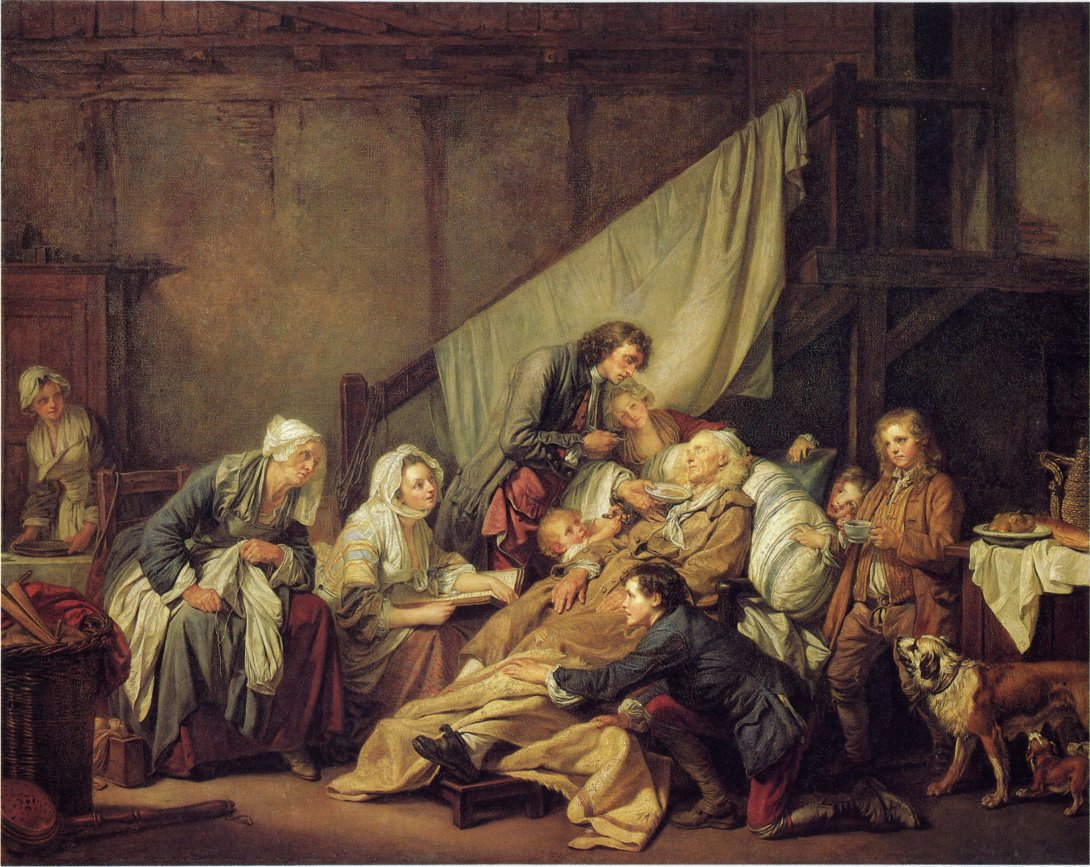
\includegraphics[angle=90, width=\linewidth]{img/GREUZE-Paralytique.jpg}
\caption{Jean-Baptiste \textsc{Greuze}, \textit{La Piété filiale} ou \textit{Le Paralytique}, 1761, Peinture sur toile, 115×146~cm, Musée de l'Ermitage, Saint-Pétersbourg.}
\end{figure}

\sujetn{%
	nomauteur=Diderot,
	prenomauteur=Denis,
	initialeprenom =D,
	particule=,
	titre = {Salon de 1763},
	semestre = \RS,
	lieu ={Amérique du Sud},
	annee =2022,
	type =,
	jour =2,
	datepub = 1763,
	ajoutref ={«~Greuze~»},
	genre =\articlel,
	corrige =,
	liencorrige={amsud_2022_2_1},
	typequn=\litt,
	typeqdeux = \phil,
	qun = {Par quelles dimensions de l'œuvre Diderot est-il touché~?},
	qdeux ={L'art ne s'adresse-t-il qu'à la sensibilité~?},
	themeprogrammequn=EXS,
	themeprogrammeqdeux=EXS}
{\chapeau{Après avoir visité une exposition organisée par l'Académie royale de peinture et de sculpture, Denis Diderot en rend compte dans le journal \emph{Correspondance littéraire}. Il s'attarde en particulier sur un tableau de Jean Baptiste Greuze intitulé \emph{La Piété filiale} (ou \emph{Le Paralytique}).}

Le genre me plaît. C'est la peinture morale. Quoi donc, le pinceau n'a-t-il pas été assez et trop longtemps consacré à la débauche et au vice~? ne devons-nous pas être satisfaits de le voir concourir enfin avec la poésie dramatique à nous toucher, à nous instruire, à nous corriger et à nous inviter à la vertu~? Courage, mon ami Greuze~! Fais de la morale en peinture, et fais-en toujours comme cela. Lorsque tu seras au moment de quitter la vie, il n'y aura aucune de tes compositions que tu ne puisses te rappeler avec plaisir. Que n'étais-tu à côté de cette jeune fille\footnote{Il s'agit d'une jeune fille, inconnue de Diderot, venue admirer le tableau de Greuze.} qui, regardant la tête de ton \emph{Paralytique}, s'écria avec une vivacité charmante~: «~ Ah, mon Dieu, comme il me touche~; mais si je le regarde encore, je crois que je vais pleurer~». Et que cette jeune fille n'était-elle la mienne~! Je l'aurais reconnue à ce mouvement. Lorsque je vis ce vieillard éloquent et pathétique, je sentis, comme elle, mon âme s'attendrir et des pleurs prêts à tomber de mes yeux.
Le tableau de la \emph{Piété filiale}\footnote{\emph{La Piété filiale} et \emph{Le Paralytique} désignent une seule et même œuvre.} a quatre pieds six pouces de large, sur trois pieds\footnote{Soit 137~cm environ de large sur~91 cm environ de haut.} de haut.

Le principal personnage, celui qui occupe le milieu de la scène, et qui fixe l'attention, est un vieillard paralytique, étendu dans son fauteuil, la tête appuyée sur un traversin, et les pieds sur un tabouret. Il est habillé. Ses jambes malades sont enveloppées d'une couverture. Il est entouré de ses enfants et de ses petits-enfants, la plupart empressés à le servir. Sa belle tête est d'un caractère si touchant~; il paraît si sensible aux services qu'on lui rend~; il a tant de peine à parler, sa voix est si faible, ses regards si tendres, son teint si pâle, qu'il faut être sans entrailles pour ne pas les sentir remuer.
\theme{peinture}\theme{art}\theme{vertu}\theme{sensibilité}\theme{morale}\theme{vie (et mort)}\theme{larmes}\theme{enfant}\theme{vieillesse}\theme{vie (et mort)!âge de la vie}\theme{famille}\theme{pitié}}

%%%%%%%%%%%%%%%%%%%%%%%%%%%%Nv-Sujet%%%%%%%%%%%%%%%%%%%%%%%%%%%%%%%%%%%%%%%%%%
\sujetn{%
	nomauteur=Giono,
	prenomauteur=Jean,
	initialeprenom =J,
	particule=,
	titre = {L'Homme qui plantait des arbres},
	semestre = \RS,
	lieu ={Amérique du Sud},
	annee =2022,
	type =,
	jour =2,
	datepub = 1953,
	ajoutref =,
	genre =\romanl,
	corrige =,
	liencorrige={amsud_2022_2_2},
	typequn=\litt,
	typeqdeux = \phil,
	qun = {Comment Giono met-il en valeur la renaissance de la région dans cet extrait~?},
	qdeux ={La nature est-elle autre chose qu'une création humaine~?},
	themeprogrammequn=EXS,
	themeprogrammeqdeux=EXS}
{\chapeau{Ce récit raconte la rencontre entre le narrateur, jeune homme d'une vingtaine d'années, et un berger solitaire, Elzéard Bouffier, retiré dans des terres désolées et arides des Alpes de Haute Provence. Une de ses seules activités est de planter des arbres sur les terres qui l'entourent.}

J'avais vu mourir trop de monde pendant cinq ans\footnote{Allusion aux années de la Première Guerre mondiale, qui ont séparé les deux hommes.} pour ne pas imaginer facilement la mort d'Elzéard Bouffier, d'autant que, lorsqu'on en a vingt, on considère les hommes de cinquante comme des vieillards à qui il ne reste plus qu'à mourir. Il n'était pas mort. Il était même fort vert. Il avait changé de métier. Il ne possédait plus que quatre brebis mais, par contre, une centaine de ruches. Il s'était débarrassé des moutons qui mettaient en péril ses plantations d'arbres. Car, me dit-il (et je le constatais), il ne s'était pas du tout soucié de la guerre. Il avait imperturbablement continué à planter.

Les chênes de 1910 avaient alors dix ans et étaient plus hauts que moi et que lui. Le spectacle était impressionnant. J'étais littéralement privé de parole et, comme lui ne parlait pas, nous passâmes tout le jour en silence à nous promener dans sa forêt. Elle avait, en trois tronçons, onze kilomètres de long et trois kilomètres dans sa plus grande largeur. Quand on se souvenait que tout était sorti des mains et de l'âme de cet homme — sans moyens techniques — on comprenait que les hommes pourraient être aussi efficaces que Dieu dans d'autres domaines que la destruction.

Il avait suivi son idée, et les hêtres qui m'arrivaient aux épaules, répandus à perte de vue, en témoignaient. Les chênes étaient drus et avaient dépassé l'âge où ils étaient à la merci des rongeurs~; quant aux desseins de la Providence\footnote{Puissance supérieure qui gouverne le monde.} elle-même, pour détruire l'œuvre créée, il lui faudrait avoir désormais recours aux cyclones. Il me montra d'admirables bosquets de bouleaux qui dataient de cinq ans, c'est-à-dire de 1915, de l'époque où je combattais à Verdun. Il leur avait fait occuper tous les fonds où il soupçonnait, avec juste raison, qu'il y avait de l'humidité presque à fleur de terre. Ils étaient tendres comme des adolescents et très décidés.

La création avait l'air, d'ailleurs, de s'opérer en chaînes. Il ne s'en souciait pas~; il poursuivait obstinément sa tâche, très simple. Mais en redescendant par le village, je vis couler de l'eau dans des ruisseaux qui, de mémoire d'homme, avaient toujours été à sec. C'était la plus formidable opération de réaction qu'il m'ait été donné de voir. Ces ruisseaux secs avaient jadis porté de l'eau, dans des temps très anciens. Certains de ces villages tristes dont j'ai parlé au début de mon récit s'étaient construits sur les emplacements d'anciens villages gallo-romains dont il restait encore des traces, dans lesquelles les archéologues avaient fouillé et ils avaient trouvé des hameçons à des endroits où au vingtième siècle, on était obligé d'avoir recours à des citernes pour avoir un peu d'eau.

Le vent aussi dispersait certaines graines. En même temps 
que l'eau réapparut réapparaissaient les saules, les osiers, les prés, les jardins, les fleurs et une certaine raison de vivre.
\theme{nature!environnement}\theme{solitude}\theme{guerre!Première Guerre mondiale}\theme{vie (et mort)}\theme{vieillesse}\theme{lyrisme}\theme{animaux}\theme{silence}\theme{berger}\theme{technique!maîtrise technique de la nature}\theme{création!humaine}\theme{renouvellement!de la nature}}

%%%%%%%%%%%%%%%%%%%%%%%%%%%%Nv-Sujet%%%%%%%%%%%%%%%%%%%%%%%%%%%%%%%%%%%%%%%%%%
\sujetn{%
	nomauteur=Camus,
	prenomauteur=Albert,
	initialeprenom =A,
	particule=,
	titre = {Noces},
	semestre = \RS,
	lieu ={Amérique du Nord},
	annee =2022,
	type =,
	jour =1,
	datepub = 1939,
	ajoutref ={«~Noces à Tipasa~»},
	genre =\romanl,
	corrige =Oui,
	liencorrige={amnord_2022_1_1},
	typequn=\litt,
	typeqdeux = \phil,
	qun = {Comment ce texte nous fait-il entendre «~la mélodie du monde~»~?},
	qdeux ={L'art réconcilie-t-il l'homme et la nature~?},
	themeprogrammequn=EXS,
	themeprogrammeqdeux=EXSMM}
{Que d'heures passées à écraser les absinthes\footnote{Absinthes,
sauges et ravenelles sont des plantes méditerranéennes.}, à caresser
les ruines, à tenter d'accorder ma respiration aux soupirs tumultueux
du monde~! Enfoncé parmi les odeurs sauvages et les concerts
d'insectes somnolents, j'ouvre les yeux et mon cœur à la grandeur
insoutenable de ce ciel gorgé de chaleur. Ce n'est pas si facile de
devenir ce qu'on est, de retrouver sa mesure profonde.

Mais à regarder l'échine solide du Chenoua\footnote{Chenoua~: Le
Chenoua est une montagne, située dans la région de Tipasa, au nord de
l'Algérie.}, mon cœur se calmait d'une étrange certitude. J'apprenais
à respirer, je m'intégrais et je m'accomplissais. Je gravissais l'un
après l'autre des coteaux dont chacun me réservait une récompense,
comme ce temple dont les colonnes mesurent la course du soleil et
d'où l'on voit le village entier, ses murs blancs et roses et ses
vérandas vertes.

Comme aussi cette basilique\footnote{Basilique~: monument de l'Église
catholique, dévoué à un saint.} sur la colline Est~: elle a gardé ses
murs et dans un grand rayon autour d'elle s'alignent des sarcophages
exhumés, pour la plupart à peine issus de la terre dont ils
participent encore. Ils ont contenu des morts~; pour le moment il y
pousse des sauges et des ravenelles.

La basilique Sainte-Salsa est chrétienne, mais à chaque fois qu'on
regarde par une ouverture, c'est la mélodie du monde qui parvient
jusqu'à nous~: coteaux plantés de pins et de cyprès, ou bien la mer
qui roule ses chiens blancs à une vingtaine de mètres. La colline qui
supporte Sainte-Salsa est plate à son sommet et le vent souffle plus
largement à travers les portiques. Sous le soleil du matin, un grand
bonheur se balance dans l'espace.
\theme{introspection!se trouver}\theme{paysage}\theme{nature!environnement}\theme{solitude}\theme{musique}}

%%%%%%%%%%%%%%%%%%%%%%%%%%%%Nv-Sujet%%%%%%%%%%%%%%%%%%%%%%%%%%%%%%%%%%%%%%%%%%
\sujetn{%
	nomauteur=Musset,
	prenomauteur=Alfred,
	initialeprenom =A,
	particule=de,
	titre = {La Nuit d'Août},
	semestre = \RS,
	lieu ={Amérique du Nord},
	annee =2022,
	type =,
	jour =2,
	datepub =1837,
	ajoutref =,
	genre =\poesie,
	corrige =Oui,
	liencorrige={amnord_2022_2_1},
	typequn=\litt,
	typeqdeux = \phil,
	qun = {En quoi le poète fait-il de la nature le reflet de sa sensibilité~?},
	qdeux ={L'art peut-il sublimer la souffrance~?},
	themeprogrammequn=EXS,
	themeprogrammeqdeux=EXS}
{\vspace*{-30pt}\par\chapeau{Dans ce poème \emph{«~La Nuit d'Août~»}, Musset présente le
dialogue entre deux personnages~: la Muse et le Poète. À la Muse qui
évoque le désenchantement de l'expérience et la déchéance de la
vieillesse, le Poète répond par ces strophes qui terminent le poème.}

\setlength{\parskip}{0pt}

Puisque l'oiseau des bois voltige et chante encore

Sur la branche où ses œufs sont brisés dans le nid~;

Puisque la fleur des champs entr'ouverte à l'aurore,

Voyant sur la pelouse une autre fleur éclore,

S'incline sans murmure et tombe avec la nuit,

Puisqu'au fond des forêts, sous les toits de verdure,

On entend le bois mort craquer dans le sentier,

Et puisqu'en traversant l'immortelle nature,

L'homme n'a su trouver de science qui dure,

Que de marcher toujours et toujours oublier~;

Puisque, jusqu'aux rochers tout se change en poussière~;

Puisque tout meurt ce soir pour revivre demain~;

Puisque c'est un engrais que le meurtre et la guerre~;

Puisque sur une tombe on voit sortir de terre

Le brin d'herbe sacré qui nous donne le pain~;

Ô Muse~! que m'importe ou la mort ou la vie~?

J'aime, et je veux pâlir~; j'aime et je veux souffrir~;

J'aime, et pour un baiser je donne mon génie~;

J'aime, et je veux sentir sur ma joue amaigrie

Ruisseler une source impossible à tarir.

J'aime, et je veux chanter la joie et la paresse,

Ma folle expérience et mes soucis d'un jour,

Et je veux raconter et répéter sans cesse

Qu'après avoir juré de vivre sans maîtresse,

J'ai fait serment de vivre et de mourir d'amour.

Dépouille devant tous l'orgueil qui te dévore,

Cœur gonflé d'amertume et qui t'es cru fermé.

Aime, et tu renaîtras~; fais-toi fleur pour éclore.

Après avoir souffert, il faut souffrir encore~;

Il faut aimer sans cesse, après avoir aimé.

\setlength{\parskip}{6pt}
\theme{nature!environnement}\theme{paysage}\theme{amour}\theme{inspiration}\theme{vie (et mort)}\theme{souffrance}\theme{nuit}}


%%%%%%%%%%%%%%%%%%%%%%%%%%%%Nv-Sujet%%%%%%%%%%%%%%%%%%%%%%%%%%%%%%%%%%%%%%%%%%
\sujetn{%
	nomauteur=Hegel,
	prenomauteur={Georg Wilhelm Friedrich},
	initialeprenom =G.~W.~F,
	particule=,
	titre = {Esthétique},
	semestre = \RS,
	lieu =Asie,
	annee =2022,
	type =,
	jour =1,
	datepub ={1818-1829},
	ajoutref ={traduction S.~\textsc{Jankélévitch}},
	genre =\essaip,
	corrige =,
	liencorrige={asi_2022_1_2},
	typequn = \phil,
	typeqdeux = \litt,
	qun = {Selon ce texte, comment la représentation artistique de nos passions permet-elle de nous en libérer~?},
	qdeux ={La littérature et les arts ont-ils vraiment un pouvoir consolateur~?},
	themeprogrammequn=EXS,
	themeprogrammeqdeux=EXS}
{Un désir est d'autant plus sauvage qu'il s'empare à lui seul de
l'homme tout entier et que l'homme n'a pas encore appris à se
différencier, en tant que généralité, par rapport à cette
détermination. Quand je dis~: ma passion est plus forte que moi, je
fais bien une différence entre mon moi abstrait et la passion~; mais
c'est là une distinction purement formelle qui signifie que je ne
suis rien en comparaison de la passion. La sauvagerie de la passion
résulte donc de l'unité qui existe entre mon moi général et la
limitation à laquelle il est soumis, de sorte que je ne connais pas
d'autre volonté que cette volonté limitée. On appelle \textit{un homme
entier}\footnote{«~un homme entier~»~: en français dans le texte.} un
homme qui concentre toute sa volonté sur une fin particulière.

C'est là la sauvagerie, force et puissance de l'homme dominé par les
passions. Elle peut être adoucie par l'art, dans la mesure où
celui-ci représente à l'homme les passions elles-mêmes, les instincts
et, en général, l'homme tel qu'il est. Et en se bornant à dérouler le
tableau des passions, l'art, alors même qu'il les flatte, le fait
pour montrer à l'homme ce qu'il est, pour l'en rendre conscient.
C'est déjà en cela que consiste son action adoucissante, car il met
ainsi l'homme en présence de ses instincts, comme s'ils étaient en
dehors de lui, et lui confère de ce fait une certaine liberté à leur
égard. Sous ce rapport, on peut dire de l'art qu'il est un
libérateur. Les passions perdent leur force, du fait même qu'elles
sont devenues objets de représentations, objets tout court.
L'objectivation\footnote{«~objectivation~»~: passage d'un vécu
intérieur à une réalité extérieure.} des sentiments a justement pour
effet de leur enlever leur intensité et de nous les rendre
extérieurs, plus ou moins étrangers. Par son passage dans la
représentation, le sentiment sort de l'état de concentration dans
lequel il se trouvait en nous et s'offre à notre libre jugement. Il
en est des passions comme de la douleur~: le premier moyen que la
nature met à notre disposition pour obtenir un soulagement d'une
douleur qui nous accable, sont les larmes~; pleurer, c'est déjà être
consolé. Le soulagement s'accentue ensuite au cours de conversations
avec des amis, et le besoin d'être soulagé et consolé peut nous
pousser jusqu'à composer des poésies. C'est ainsi que dès qu'un homme
qui se trouve plongé dans la douleur et absorbé par elle est à même
d'extérioriser cette douleur, il s'en sent soulagé, et ce qui soulage
encore davantage, c'est son expression en paroles, en chants, en sons
et en figures. Ce dernier moyen est encore plus efficace.
\theme{désir}\theme{identité!et différences}\theme{passion}\theme{moi!moi abstrait}\theme{art}\theme{liberté}\theme{émotions!objectivation des émotions}\theme{souffrance}\theme{consolation}\theme{sentiments}\theme{larmes}}

%%%%%%%%%%%%%%%%%%%%%%%%%%%%Nv-Sujet%%%%%%%%%%%%%%%%%%%%%%%%%%%%%%%%%%%%%%%%%%

\sujetn{%
	nomauteur=Dumas,
	prenomauteur=Alexandre,
	initialeprenom =A,
	particule=,
	titre = {Kean},
	semestre = \RS,
	lieu =Asie,
	annee =2022,
	type =,
	jour =2,
	datepub = 1836,
	ajoutref ={acte II, scène 4},
	genre =\theatre,
	corrige =,
	liencorrige={asi_2022_2_1},
	typequn=\litt,
	typeqdeux = \phil,
	qun = {Comment la personnalité de Kean est-elle liée à son métier d'acteur~?},
	qdeux ={Jouer un rôle, est-ce trahir son identité~?},
	themeprogrammequn=EXSMM,
	themeprogrammeqdeux=MM}
{\chapeau{
Dans cette scène, Kean, un célèbre acteur, conseille la jeune Anna qui
souhaite devenir comédienne.}

\vspace*{-18pt}\personnage{KEAN.}

Oui, je suis roi, c'est vrai… trois fois par semaine à peu près, roi
avec un sceptre de bois doré, des diamants de strass et une couronne
de carton~; j'ai un royaume de trente-cinq pieds carrés, et une
royauté qu'un bon petit coup de sifflet fait évanouir. Oh~! oui, oui,
je suis un roi bien respecté, bien puissant, et surtout bien heureux,
allez~!

\personnage{ANNA.}

Ainsi, lorsque tout le monde vous applaudit, vous envie, vous admire…

\personnage{KEAN.}

Eh bien~! parfois, je blasphème, je maudis, je jalouse le sort du
portefaix\footnote{“portefaix”~: celui dont le métier consiste à
porter des fardeaux}, courbé sous son fardeau… du laboureur sur sa
charrue, et du marin couché sur le pont du vaisseau.

\personnage{ANNA.}

Et si une femme, jeune, riche, et qui vous aimât, venait vous dire~:
Kean, ma fortune, mon amour, sont à vous… sortez de cet enfer qui
vous brûle… de cette existence qui vous dévore… quittez le théâtre…

\personnage{KEAN.}

Moi~! moi~! quitter le théâtre… moi~! Oh~! vous ne savez donc pas ce
que c'est que cette robe de Nessus\footnote{“robe de Nessus”~:
tunique empoisonnée reçue en cadeau par Hercule et qui lui brûle la
peau} qu'on ne peut arracher de dessus ses épaules qu'en déchirant sa
propre chair~: moi, quitter le théâtre, renoncer à ses émotions, à
ses éblouissements, à ses douleurs~! moi, céder la place à Kemble et
à Macready\footnote{“à Kemble et à Macready”~: acteurs rivaux de
Kean}, pour qu'on m'oublie au bout d'un an, au bout de six mois,
peut-être~! Mais rappelez-vous donc que l'acteur ne laisse rien après
lui, qu'il ne vit que pendant sa vie, que sa mémoire s'en va avec la
génération à laquelle il appartient, et qu'il tombe du jour dans la
nuit… du trône dans le néant… Non~! non~! lorsqu'on a mis le pied une
fois dans cette fatale carrière, il faut la parcourir jusqu'au bout…,
épuiser ses joies et ses douleurs, vider sa coupe et son
calice\footnote{“calice”~: vase sacré}, boire son miel et sa
lie\footnote{“lie”~: dépôt amer du vin}… Il faut finir comme on a
commencé, mourir comme on a vécu… mourir comme est mort Molière, au
bruit des applaudissements, des sifflets et des bravos~!… Mais
lorsqu'il est encore temps de ne pas prendre cette route, lorsqu'on
n'a pas franchi la barrière… il n'y faut pas… croyez-moi,
\textit{miss}, sur mon honneur~! croyez-moi.
\theme{théâtre}\theme{souvenir}\theme{identité!sociale}\theme{mensonge}\theme{rôle!jouer un rôle}\theme{mémoire}}

%%%%%%%%%%%%%%%%%%%%%%%%%%%%Nv-Sujet%%%%%%%%%%%%%%%%%%%%%%%%%%%%%%%%%%%%%%%%%%
\sujetn{%
	nomauteur=Proust,
	prenomauteur=Marcel,
	initialeprenom =M,
	particule=,
	titre = {Du côté de chez Swann},
	semestre = \RS,
	lieu ={Centres étrangers},
	annee =2022,
	type =,
	jour =1,
	datepub =1913,
	ajoutref =,
	genre =\romanl,
	corrige =Oui,
	liencorrige={cea_2022_1_2},
	typequn=\litt,
	typeqdeux = \phil,
	qun = {En quoi l'identité du personnage de Swann se métamorphose-t-elle~?},
	qdeux ={Notre personnalité sociale n'est-elle qu'une création de la pensée des autres~?},
	themeprogrammequn=MM,
	themeprogrammeqdeux=MM}
{Mais même au point de vue des plus insignifiantes choses de la vie,
nous ne sommes pas un tout matériellement constitué, identique pour
tout le monde et dont chacun n'a qu'à aller prendre connaissance
comme d'un cahier des charges ou d'un testament~; notre personnalité
sociale est une création de la pensée des autres. Même l'acte si
simple que nous appelons «~voir une personne que nous connaissons~»
est en partie un acte intellectuel. Nous remplissons l'apparence
physique de l'être que nous voyons de toutes les notions que nous
avons sur lui, et dans l'aspect total que nous nous représentons, ces
notions ont certainement la plus grande part. Elles finissent par
gonfler si parfaitement les joues, par suivre en une adhérence si
exacte la ligne du nez, elles se mêlent si bien de nuancer la
sonorité de la voix comme si celle-ci n'était qu'une transparente
enveloppe, que chaque fois que nous voyons ce visage et que nous
entendons cette voix, ce sont ces notions que nous retrouvons, que
nous écoutons. Sans doute, dans le Swann qu'ils s'étaient constitué,
mes parents avaient omis par ignorance de faire entrer une foule de
particularités de sa vie mondaine qui étaient cause que d'autres
personnes, quand elles étaient en sa présence, voyaient les élégances
régner dans son visage et s'arrêter à son nez busqué comme à leur
frontière naturelle~; mais aussi ils avaient pu entasser dans ce
visage désaffecté de son prestige, vacant et spacieux, au fond de ces
yeux dépréciés, le vague et doux résidu – mi-mémoire, mi-oubli – des
heures oisives passées ensemble après nos dîners hebdomadaires,
autour de la table de jeu ou au jardin, durant notre vie de bon
voisinage campagnard. L'enveloppe corporelle de notre ami en avait
été si bien bourrée, ainsi que de quelques souvenirs relatifs à ses
parents, que ce Swann-là était devenu un être complet et vivant, et
que j'ai l'impression de quitter une personne pour aller vers une
autre qui en est distincte, quand, dans ma mémoire, du Swann que j'ai
connu plus tard avec exactitude, je passe à ce premier Swann – à ce
premier Swann dans lequel je retrouve les erreurs charmantes de ma
jeunesse et qui d'ailleurs ressemble moins à l'autre qu'aux personnes
que j'ai connues à la même époque, comme s'il en était de notre vie
ainsi que d'un musée où tous les portraits d'un même temps ont un air
de famille, une même tonalité – à ce premier Swann rempli de loisir,
parfumé par l'odeur du grand marronnier, des paniers de framboises et
d'un brin d'estragon.
\theme{identité!sociale}\theme{moi!fragmentation du moi}\theme{autrui}\theme{reconnaissance}\theme{corps}\theme{identité!et changements}\theme{mémoire}\theme{oubli}}

%%%%%%%%%%%%%%%%%%%%%%%%%%%%Nv-Sujet%%%%%%%%%%%%%%%%%%%%%%%%%%%%%%%%%%%%%%%%%%

\sujetn{%
	nomauteur=Chateaubriand,
	prenomauteur={François-René},
	initialeprenom ={F.-R},
	particule=de,
	titre = {Mémoires d'outre-tombe},
	semestre = \RS,
	lieu = {Centres étrangers},
	annee =2022,
	type =,
	jour =2,
	datepub ={1809-1841},
	ajoutref = {livre troisième, chapitre IV},
	genre =\memoire,
	corrige =Oui,
	liencorrige={cea_2022_2_1},
	typequn=\litt,
	typeqdeux = \phil,
	qun = {Comment l'auteur s'approprie-t-il une expérience de l'enfance~?},
	qdeux ={La sensibilité est-elle formée par les seules épreuves de la vie~?},
	themeprogrammequn=MM,
	themeprogrammeqdeux=EXSMM}
{Quelques martinets, qui durant l'été s'enfonçaient en criant dans les
trous des murs, étaient mes seuls compagnons. La nuit, je
n'apercevais qu'un petit morceau de ciel et quelques étoiles. Lorsque
la lune brillait et qu'elle s'abaissait à l'occident, j'en étais
averti par ses rayons, qui venaient à mon lit au travers des carreaux
losangés de la fenêtre. Des chouettes, voletant d'une tour à l'autre,
passant et repassant entre la lune et moi, dessinaient sur mes
rideaux l'ombre mobile de leurs ailes. Relégué dans l'endroit le plus
désert, à l'ouverture des galeries, je ne perdais pas un murmure des
ténèbres. Quelquefois le vent semblait courir à pas légers~;
quelquefois il laissait échapper des plaintes~; tout à coup ma porte
était ébranlée avec violence, les souterrains poussaient des
mugissements, puis ces bruits expiraient pour recommencer encore. À
quatre heures du matin, la voix du maître du château, appelant le
valet de chambre à l'entrée des voûtes séculaires, se faisait
entendre comme la voix du dernier fantôme de la nuit. Cette voix
remplaçait pour moi la douce harmonie au son de laquelle le père de
Montaigne éveillait son fils.

L'entêtement du comte de Chateaubriand à faire coucher un enfant seul
au haut d'une tour pouvait avoir quelque inconvénient~; mais il
tourna à mon avantage. Cette manière violente de me traiter me laissa
le courage d'un homme, sans m'ôter cette sensibilité d'imagination
dont on voudrait aujourd'hui priver la jeunesse. Au lieu de chercher
à me convaincre qu'il n'y avait point de revenants, on me força de
les braver. Lorsque mon père me disait, avec un sourire ironique~:
«~Monsieur le chevalier aurait-il peur~?~» il m'eût fait coucher avec
un mort. Lorsque mon excellente mère me disait~: «~Mon enfant, tout
n'arrive que par la permission de Dieu~; vous n'avez rien à craindre
des mauvais esprits, tant que vous serez bon chrétien~;~» j'étais
mieux rassuré que par tous les arguments de la philosophie. Mon
succès fut si complet que les vents de la nuit, dans ma tour
déshabitée, ne servaient que de jouets à mes caprices et d'ailes à
mes songes. Mon imagination allumée, se propageant sur tous les
objets, ne trouvait nulle part assez de nourriture et aurait dévoré
la terre et le ciel.
\theme{nature!environnement}\theme{paysage}\theme{solitude}\theme{nuit}\theme{imagination}\theme{enfant}\theme{sensibilité}\theme{vie (et mort)!âge de la vie}}

%%%%%%%%%%%%%%%%%%%%%%%%%%%%Nv-Sujet%%%%%%%%%%%%%%%%%%%%%%%%%%%%%%%%%%%%%%%%%%

\sujetn{%
	nomauteur=Verlaine,
	prenomauteur=Paul,
	initialeprenom =P,
	particule=,
	titre = {Fêtes galantes},
	semestre = \RS,
	lieu =Liban,
	annee =2022,
	type =,
	jour =1,
	datepub =1869,
	ajoutref =,
	genre =\poesie,
	corrige =,
	liencorrige={lib2022_1_1},
	typequn=\litt,
	typeqdeux = \phil,
	qun = {Quelle image ce poème donne-t-il de la relation amoureuse~?},
	qdeux ={Nos sentiments résistent-ils au temps~?},
	themeprogrammequn=EXS,
	themeprogrammeqdeux=EXSMM}
{\begin{center}COLLOQUE SENTIMENTAL\end{center}

\setlength{\parskip}{0pt}

\bigskip

Dans le vieux parc solitaire et glacé

Deux formes ont tout à l'heure passé.

\medskip

Leurs yeux sont morts et leurs lèvres sont molles,

Et l'on entend à peine leurs paroles.

\medskip

Dans le vieux parc solitaire et glacé

Deux spectres ont évoqué le passé.

\medskip

—~Te souvient-il de notre extase ancienne~?

—~Pourquoi voulez-vous donc qu'il m'en souvienne~?

\medskip

—~Ton cœur bat-il toujours à mon seul nom~?

Toujours vois-tu mon âme en rêve~? – Non.

\medskip

—~Ah~! les beaux jours de bonheur indicible

Où nous joignions nos bouches~! – C'est possible.

\medskip

—~Qu'il était bleu, le ciel, et grand, l'espoir~!

—~L'espoir a fui, vaincu, vers le ciel noir.

\medskip

Tels ils marchaient dans les avoines folles,

Et la nuit seule entendit leurs paroles.

\setlength{\parskip}{6pt}
\theme{amour}\theme{souvenir}\theme{oubli}\theme{nuit}\theme{solitude}\theme{sentiments}}

%%%%%%%%%%%%%%%%%%%%%%%%%%%%Nv-Sujet%%%%%%%%%%%%%%%%%%%%%%%%%%%%%%%%%%%%%%%%%%

\sujetn{%
	nomauteur=Noailles,
	prenomauteur={Anna},
	initialeprenom={A},
	particule=de,
	titre = {Le visage émerveillé},
	semestre = \RS,
	lieu =Liban,
	annee =2022,
	type =,
	jour =2,
	datepub =1904,
	ajoutref =,
	genre =\romanl,
	corrige =,
	liencorrige={lib2022_2_1},
	typequn=\litt,
	typeqdeux = \phil,
	qun = {Peut-on dire que le personnage de Sophie est dominé par sa sensibilité~?},
	qdeux ={Nos choix de vie peuvent-ils se faire contre nos sentiments~?},
	themeprogrammequn=EXS,
	themeprogrammeqdeux=EXS}
{\chapeau{
La sœur Sainte-Sophie vit dans un couvent depuis deux ans, parce
qu'elle «~aime Dieu, la mère abbesse, le silence~». Un jeune homme,
Julien, vient admirer un tableau dans la chapelle du couvent. C'est
le coup de foudre mais, au nom de sa foi, Sophie décide de renoncer à
Julien.}

{\raggedleft
10 décembre.
\par}

Mon chéri, voilà plus de trois semaines que je suis malade. On ne me
donne pas vos lettres, et si je vous écrivais, on ne vous ferait pas
parvenir les miennes.

Je n'ai plus de force, je voudrais beaucoup mourir. Par moments, je
vous vois comme si vous étiez très loin, je n'entends presque plus
votre voix, et à d'autres instants votre image emplit et déchire mon
cœur resserré. Je ne sais si je redoute ou si je souhaite que vous
vous effaciez en moi.

Tout ce qu'on peut souffrir, je l'ai souffert~: j'ai pensé m'éteindre
de violence et de colère, et maintenant je souffre d'une douce et
terrible sentimentalité~; ce sentiment fait plus mal que les autres~;
je pense à vous avec une tendresse qui me tue. Je suis là, couchée,
près de la sœur Marthe qui brode. Je vois par la fenêtre un ciel
d'hiver très bleu.

Si je n'avais connu que votre passion et la mienne, je pourrais,
aujourd'hui où je suis si malade, oublier, mais j'ai connu, mon
chéri, votre bonté.

J'ai connu votre bonté pour moi auprès de laquelle l'affection de la
supérieure est pauvre et blessante, la sympathie de mes sœurs
misérable.

Vous m'avez tant donné, dans des moments de douceur sans limite, que
l'attention moindre de toutes les autres âmes ne peut plus que
m'offenser. La pureté, l'amitié infinie, c'est nous qui les avons
goûtées, dans les instants où, sans secret, sans défiance, nous fûmes
vraiment des âmes mêlées, des regards pareils. Que les amies
parfaites aient entre elles besoin de précautions et d'égards, que
les frères et les parents se respectent et craignent de s'offenser,
mais nous, quels soins eussions-nous pu prendre d'une âme qui nous
était commune~?

Je me souviens que vous sembliez oppressé la nuit où vous m'avez
quittée.

Hélas~! je n'ai pas suivi votre douleur. Comment étiez-vous quand vous
êtes rentré dans votre chambre, quand vos bras pendaient le long de
votre corps, quand vous vous êtes assis avec stupeur, car les hommes,
n'est-ce pas, sont étonnés de souffrir~? Mon chéri, cette
sentimentalité dont la douceur fait mal, je ne puis l'écarter de moi,
elle pèse sur mon cœur et m'étouffe, comme ces beaux chats chauds et
fourrés qui s'endorment la nuit sur la poitrine des petits enfants.
\theme{amour}\theme{vie (et mort)}\theme{émotions}\theme{passion}\theme{sentiments}\theme{souffrance}\theme{religion}\theme{sensibilité}\theme{maladie}}

%%%%%%%%%%%%%%%%%%%%%%%%%%%%Nv-Sujet%%%%%%%%%%%%%%%%%%%%%%%%%%%%%%%%%%%%%%%%%%

\sujetn{%
	nomauteur=Albert-Birot,
	prenomauteur=Pierre,
	initialeprenom ={P},
	titre = {Poésies},
	semestre = \RS,
	lieu =Métropole,
	annee =2022,
	type =,
	jour =1,
	datepub =1926,
	ajoutref =«~L'affaire Narcisse~»,
	genre =\poesie,
	corrige =Oui,
	liencorrige={met_2022_1_1},
	typequn=\litt,
	typeqdeux = \phil,
	qun = {«~L'affaire Narcisse~»~: comment votre lecture du poème éclaire-t-elle ce titre~?},
	qdeux ={Se connaître soi-même, est-ce se découvrir «~pièce unique~»~?},
	themeprogrammequn=OdS,
	themeprogrammeqdeux=MM}
{%
\begin{center}
L'AFFAIRE NARCISSE
\end{center}

\setlength{\parskip}{0pt}

\bigskip

Narcisse fils de Céphise\footnote{Personnage de la mythologie grecque, fils de la nymphe Liriope et du fleuve Céphise, Narcisse est doté d'une grande beauté. Indifférent à l'admiration qu'on lui voue, il aperçoit un jour son reflet dans l'eau et en tombe amoureux. A force d'auto-contemplation, il finit par mourir, et est métamorphosé en fleur.} n'est plus depuis des montagnes de temps

En nos âges il n'est plus de ces Narcisse-là

Seule une fleur nous reste

Et pourtant nous avons des miroirs autrement plus parfaits que la
fontaine

Où s'admira ce trop joli garçon

Ne dirai point que ne suis jamais venu devant ma glace

Au cours de mon printemps de mon été même des froides saisons qui
suivent

Mais pas une fois ne me suis dit celui-là c'est moi

Or bien hier

Sans doute disons

Glace parfaite

Lumière magnifique

Et temps à perdre

Celui-là fut moi

Je l'ai vu totalement vu

Et j'ai dû me dire et me redire tant que j'ai pu

Cet homme qui est là devant c'est toi complètement toi

De la tête aux pieds et quelle découverte moi je suis fait comme tout
homme est fait

Et pourtant ne ressemble à aucun

Toutefois ne sais si vais m'aimer autant que je m'aimais avant de me
connaître

Enfin c'est agréable tout de même de se savoir pièce unique

Et n'oublions pas que chaque être humain peut en dire autant

A bien regarder Narcisse avait raison

Un homme ça vaut la peine d'être vu

\setlength{\parskip}{6pt}
\theme{narcissisme}\theme{contemplation}\theme{reconnaissance}\theme{corps}\theme{identité}\theme{identité!comme unicité}\theme{introspection}}

%%%%%%%%%%%%%%%%%%%%%%%%%%%%Nv-Sujet%%%%%%%%%%%%%%%%%%%%%%%%%%%%%%%%%%%%%%%%%%

\sujetn{%
	nomauteur=Rousseau,
	prenomauteur=Jean-Jacques,
	initialeprenom ={J.-J},
	titre = {Lettres morales},
	semestre = \RS,
	lieu =Métropole,
	annee =2022,
	type =,
	jour =2,
	datepub =1758,
	ajoutref ={Lettre VI},
	genre =\lettrep,
	corrige =Oui,
	liencorrige={met_2022_2_1},
	typequn = \phil,
	typeqdeux = \litt,
	qun = {Dans quelle mesure pouvons-nous redevenir nous-mêmes~?},
	qdeux ={Lire permet-il d'accéder à une meilleure connaissance de soi~?},
	themeprogrammequn=MM,
	themeprogrammeqdeux=MM}
{Quand je vois chacun de nous sans cesse occupé de l'opinion publique
étendre pour ainsi dire son existence tout autour de lui sans en
réserver presque rien dans son propre cœur, je crois voir un petit
insecte former de sa substance une grande toile par laquelle seule il
paraît sensible tandis qu'on le croirait mort dans son trou. La
vanité de l'homme est la toile d'araignée qu'il tend sur tout ce qui
l'environne. L'une est aussi solide que l'autre, le moindre fil qu'on
touche met l'insecte en mouvement, il mourrait de langueur si l'on
laissait la toile tranquille, et si d'un doigt on la déchire il
achève de s'épuiser plutôt que de ne la pas refaire à l'instant.
Commençons par redevenir nous, par nous concentrer en nous, par
circonscrire notre âme des mêmes bornes que la nature a données à
notre être, commençons en un mot par nous rassembler où nous sommes,
afin qu'en cherchant à nous connaître tout ce qui nous compose vienne
à la fois se présenter à nous. Pour moi, je pense que celui qui sait
le mieux en quoi consiste le moi humain est le plus près de la
sagesse et que comme le premier trait d'un dessin se forme des lignes
qui le terminent, la première idée de l'homme est de le séparer de
tout ce qui n'est pas lui.

Mais comment se fait cette séparation~? Cet art n'est pas si difficile
qu'on pourrait croire, ou du moins la difficulté n'est pas où on la
croit, il dépend plus de la volonté que des lumières, il ne faut
point un appareil d'études et de recherches pour y parvenir. Le jour
nous éclaire, et le miroir est devant nous~; mais pour le voir il
faut jeter les yeux et le moyen de les y fixer est d'écarter les
objets qui nous en détournent. Recueillez-vous, cherchez la solitude,
voilà d'abord tout le secret et par celui-là seul on découvre bientôt
les vôtres. Pensez-vous en effet que la philosophie nous apprenne à
rentrer en nous – mêmes~? Ah combien l'orgueil sous son nom nous en
écarte~! C'est tout le contraire ma charmante amie, il faut commencer
par rentrer en soi pour apprendre à philosopher.
\theme{identité!sociale}\theme{rôle!jouer un rôle}\theme{moi!unité du moi}\theme{nature!nature humaine}\theme{soi!difficile accès à soi}\theme{solitude}\theme{philosophie}\theme{moi!frontières du moi}}

%%%%%%%%%%%%%%%%%%%%%%%%%%%%%Nv-Sujet%%%%%%%%%%%%%%%%%%%%%%%%%%%%%%%%%%%%%%%%

\sujetn{%
	nomauteur=Maupassant,
	prenomauteur={Guy},
	initialeprenom ={G},
	particule=de,
	titre = {Fort comme la mort},
	semestre = \RS,
	lieu =Métropole,
	annee =2022,
	type =Remplacement,
	jour =1,
	datepub =1889,
	ajoutref =,
	genre =\romanl,
	corrige =Oui,
	liencorrige={metrem_2022_1_2},
	typequn=\litt,
	typeqdeux = \phil,
	qun = {Que révèle ici la métamorphose physique~?},
	qdeux ={La souffrance a-t-elle un effet sur ce que je suis~?},
	themeprogrammequn=MM,
	themeprogrammeqdeux=EXSMM}
{Elle se croyait même au début d'une période heureuse et tranquille quand la mort de sa mère vint la frapper en plein cœur. Ce fut, pendant les premiers jours, un de ces désespoirs profonds qui ne laissent place à nulle autre pensée. Elle restait du matin au soir abîmée dans la désolation, cherchant à se rappeler mille choses de la morte, des paroles familières, sa figure d'autrefois, des robes qu'elle avait portées jadis, comme si elle eût amassé au fond de sa mémoire des reliques, et recueilli dans le passé disparu tous les intimes et menus souvenirs dont elle alimenterait ses cruelles rêveries. Puis quand elle fut arrivée ainsi à un tel paroxysme\footnote{«~paroxysme~»~: stade le plus élevé.} de désespoir, qu'elle avait à tout instant des crises de nerfs et des syncopes\footnote{«~syncopes~»~: pertes de connaissance.}, toute cette peine accumulée jaillit en larmes, et, jour et nuit, coula de ses yeux.

Or, un matin, comme sa femme de chambre entrait et venait d'ouvrir les volets et les rideaux en demandant~: «~Comment va Madame aujourd'hui~?~», elle répondit, se sentant épuisée et courbaturée à force d'avoir pleuré~: «~Oh, pas du tout. Vraiment, je n'en puis plus.~» La domestique qui tenait le plateau portant le thé regarda sa maîtresse, et émue de la voir si pâle dans la blancheur du lit, elle balbutia avec un accent triste et sincère~:

— En effet, Madame a très mauvaise mine. Madame ferait bien de se soigner.

Le ton dont cela fut dit enfonça au cœur de la comtesse une petite piqûre comme d'une pointe d'aiguille, et dès que la bonne fut partie, elle se leva pour aller voir sa figure dans sa grande armoire à glace.

Elle demeura stupéfaite en face d'elle-même, effrayée de ses joues creuses, de ses yeux rouges, du ravage produit sur elle par ces quelques jours de souffrance. Son visage qu'elle connaissait si bien, qu'elle avait si souvent regardé en tant de miroirs divers, dont elle savait toutes les expressions, toutes les gentillesses, tous les sourires, dont elle avait déjà bien des fois corrigé la pâleur, réparé les petites fatigues, détruit les rides légères apparues au trop grand jour, au coin des yeux, lui sembla tout à coup celui d'une autre femme, un visage nouveau qui se décomposait, irréparablement malade.

Pour se mieux voir, pour mieux constater ce mal inattendu, elle s'approcha jusqu'à toucher la glace du front, si près que son haleine, répandant une buée sur le verre, obscurcit, effaça presque l'image blême qu'elle contemplait. Elle dut alors prendre un mouchoir pour essuyer la brume de son souffle, et frissonnante d'une émotion bizarre, elle fit un long et patient examen des altérations de son visage. D'un doigt léger elle tendit la peau des joues, lissa celle du front, releva les cheveux, retourna les paupières pour regarder le blanc de l'œil. Puis elle ouvrit la bouche, inspecta ses dents un peu ternies où des points d'or brillaient, s'inquiéta des gencives livides et de la teinte jaune de la chair au-dessus des joues et sur les tempes.

Elle mettait à cette revue de la beauté défaillante tant d'attention qu'elle n'entendit pas ouvrir la porte, et qu'elle tressaillit jusqu'au cœur quand sa femme de chambre, debout derrière elle, lui dit~:

— Madame a oublié de prendre son thé.

La comtesse se retourna, confuse, surprise, honteuse, et la domestique, devinant sa pensée, reprit~:

— Madame a trop pleuré, il n'y a rien de pire que les larmes pour vider la peau. C'est le sang qui tourne en eau.
\theme{souffrance}\theme{tristesse}\theme{deuil}\theme{larmes}\theme{maladie}\theme{mémoire}\theme{souvenir}}

%%%%%%%%%%%%%%%%%%%%%%%%%%%%%Nv-Sujet%%%%%%%%%%%%%%%%%%%%%%%%%%%%%%%%%%%%%%%%%
\sujetn{%
	nomauteur=Rilke,
	prenomauteur=Rainer Maria,
	initialeprenom ={R.~M},
	particule=,
	titre = {Lettres à un jeune poète},
	semestre = \RS,
	lieu =Métropole,
	annee =2022,
	type =Remplacement,
	jour =2,
	datepub =1929,
	ajoutref ={trad. C.~\textsc{Mouchard}},
	genre =\lettrel,
	corrige =Oui,
	liencorrige={metrem_2022_2_2},
	typequn=\litt,
	typeqdeux = \phil,
	qun = {D'après ce texte, comment la tristesse nous transforme-t-elle~?},
	qdeux ={Se connaître est-ce comprendre ce que l'on ressent~?},
	themeprogrammequn=EXSMM,
	themeprogrammeqdeux=EXSMM}
{\chapeau{Rainer Maria Rilke s'adresse au «~jeune poète~» Franz Kappus.}

Vous avez eu maintes grandes tristesses, qui ont passé. Et vous dites que c'est aussi ce caractère passager qui vous a été pénible et contrariant. Mais réfléchissez, je vous prie~: ces grandes tristesses ne vous ont-elles pas plutôt centralement traversé~? Maintes choses en vous ne se sont-elles pas transformées, n'avez-vous pas changé en tel point, tel endroit de votre être, tandis que vous étiez triste~? Seules sont dangereuses et mauvaises les tristesses qu'on emporte au milieu des gens pour en couvrir la voix~; comme des maladies superficiellement et sottement traitées, elles ne font que reculer, et leur éruption, après une petite pause, est d'autant plus effroyable~; elles s'accumulent au-dedans, elles sont de la vie, de la vie non vécue, rejetée, perdue, de la vie dont on peut mourir. S'il nous était possible de voir un peu plus loin que notre savoir ne porte, et encore un peu au-delà des avant-postes de notre intuition, peut-être supporterions-nous alors nos tristesses avec plus de confiance que nos joies. Car elles sont les instants où quelque chose de nouveau est entré en nous, quelque chose d'inconnu~; nos sentiments se taisent, en une réticence craintive, tout en nous recule, il se fait un silence, et le nouveau, que personne ne connaît, se tient là, au milieu, muet.

Je crois que presque toutes nos tristesses sont des moments de tension que nous ressentons comme de la paralysie, sourds que nous sommes à la vie de nos sentiments frappés d'étrangeté. C'est que nous sommes seuls avec l'étranger qui est entré en nous~; c'est que tout le familier, tout l'habituel nous est pour un instant enlevé~; et que nous nous trouvons au milieu d'une transition où nous ne pouvons rester arrêtés. Voilà pourquoi la tristesse est passagère~: le nouveau en nous, venu s'ajouter, est entré dans notre cœur, a pénétré dans sa loge la plus intime, mais, là même, il n'est plus – est déjà dans le sang. Et nous n'avons pas connaissance de ce que c'était. On pourrait facilement nous faire croire que rien ne s'est passé~; et pourtant nous nous sommes transformés comme se transforme une maison où un hôte est entré. Nous ne pouvons dire qui est venu, nous ne le saurons peut-être jamais, mais bien des indices donnent à penser que c'est l'avenir qui, de cette manière, entre en nous, pour se transformer en nous, longtemps avant que de survenir.
\theme{tristesse}\theme{temps!éphémère}\theme{poésie}\theme{vie (et mort)}\theme{émotions}\theme{création}\theme{nouveauté}\theme{intime}\theme{avenir}\theme{inconnu}}

%%%%%%%%%%%%%%%%%%%%%%%%%%%%Nv-Sujet%%%%%%%%%%%%%%%%%%%%%%%%%%%%%%%%%%%%%%%%%%
\sujetn{%
	nomauteur=Présumey,
	prenomauteur=Pierre,
	initialeprenom =P,
	particule=,
	titre = {Tout ce qu'on peut},
	semestre = \RS,
	lieu =Nouvelle-Calédonie,
	annee =2022,
	type =,
	jour =2,
	datepub =2015,
	ajoutref =,
	genre =\poesie,
	corrige =,
	liencorrige={nca2022_2_1},
	typequn=\litt,
	typeqdeux = \phil,
	qun = {Le titre rend-il bien compte du poème~?},
	qdeux ={Jusqu'à quel point peut-on connaître la vie d'un homme~?},
	themeprogrammequn=OdS,
	themeprogrammeqdeux=MM}
{\vspace{-12pt}
\begin{center}
Tout ce qu'on peut
\end{center}
\setlength{\parskip}{0pt}

\medskip

On ne peut pas tenir entre ses mains la vie

D'un homme comme on tiendrait une valise pleine,

Comme on tiendrait un fagot de branches mortes,

Comme on tiendrait une pile de draps blancs,

Un panier de cerises, une corbeille de reines-claudes,

Comme on tiendrait dans son regard du haut

De la montagne tout un pays avec ses fleuves,

Avec ses collines désirables, avec ses plaines

Bien tracées~; on ne peut pas tenir entre

Ses mains la vie d'un homme tout entier

De sa chute dans le temps, à sa chute

Hors du temps, de son entrée dans la lumière

A sa sortie de la lumière~; on ne peut pas.

Tout ce qu'on peut c'est

Redire deux ou trois mots qu'il avait coutume

De dire au moment de se jeter dans le vent,

Manger les miettes du pain qu'il mangeait en partant,

Repasser son regard entre les rives où

Son regard passait, parce que c'était là

Que ses mains tenaient leur pays tout entier,

Comme un fagot de branches sèches,

Comme une pile de draps blancs bien repassés,

Comme un panier de cerises, c'était là que,

Tombé dans le temps, il mettait sa vie

Dans ses mains comme on remplit toute

Une corbeille de reines-claudes, cela

C'est tout ce qu'on peut pour le moment.

\begin{flushright}
(5 décembre 2012)\hspace*{3cm}
\end{flushright}

\setlength{\parskip}{6pt}
\theme{vie (et mort)}\theme{mort}\theme{temps}\theme{nature!environnement}\theme{mémoire}\theme{souvenir}\theme{lumière}\theme{naissance}\theme{vie (et mort)!fin de vie}\theme{temps!passage du temps}\theme{vie (et mort)!âge de la vie}\theme{autrui!comme inconnu}\theme{finitude}\theme{paysage}\theme{mémoire}\theme{souvenir}\theme{identité}\theme{existence}\theme{transmission}\theme{héritage}}

%%%%%%%%%%%%%%%%%%%%%%%%%%%%Nv-Sujet%%%%%%%%%%%%%%%%%%%%%%%%%%%%%%%%%%%%%%%%%%

\sujetn{%
	nomauteur=Beauvoir,
	prenomauteur=Simone,
	initialeprenom =S,
	particule =de,
	titre = {Mémoires d'une jeune fille rangée},
	semestre = \RS,
	lieu =Polynésie,
	annee =2022,
	type =,
	jour =1,
	datepub =1958,
	ajoutref =,
	genre =\autobiographie,
	corrige =,
	liencorrige={pol2022_1_1},
	typequn=\litt,
	typeqdeux = \phil,
	qun = {Pourquoi le passage de l'enfance à l'âge adulte effraie-t-il Simone de Beauvoir~?},
	qdeux ={Est-on le même à tous les âges de la vie~?},
	themeprogrammequn=MM,
	themeprogrammeqdeux=MM}
{Par les beaux jours d'été, il\footnote{Il s'agit du père de Simone de
Beauvoir} nous emmenait parfois, après le dîner, faire un tour au
Luxembourg\footnote{Le Jardin du Luxembourg qui jouxte le Sénat à
Paris.}~: nous mangions des glaces, à une terrasse de la place
Médicis, et, nous traversions à nouveau le jardin dont la sonnerie
d'un clairon annonçait la fermeture. J'enviais aux habitants du Sénat
leurs rêveries nocturnes, dans les allées désertes. La routine de mes
journées avait autant de rigueur que le rythme des saisons~: le
moindre écart me jetait dans l'extraordinaire. Marcher dans la
douceur du crépuscule, à l'heure où d'habitude maman verrouillait la
porte d'entrée, c'était aussi surprenant, aussi poétique qu'au cœur
de l'hiver une aubépine en fleur.

Il y eut un soir tout à fait insolite où nous bûmes un chocolat à la
terrasse de Prévost, face à l'immeuble du \textit{Matin}\footnote{Le
Matin, journal quotidien créé en 1883.}. Un journal lumineux
annonçait les péripéties du match qui se déroulait à New York entre
Carpentier et Dempsey\footnote{Allusion au «~combat du siècle~» entre
les champions de boxe Jack Dempsey et Georges Carpentier, le 2
juillet 1921.}. Le carrefour était noir de monde. Quand Carpentier
fut mis K.-O., il y eut des hommes et des femmes qui fondirent en
larmes~; je rentrai à la maison toute fière d'avoir assisté à ce
grand événement. Mais je n'aimais pas moins nos soirées quotidiennes
dans le bureau calfeutré~; mon père nous lisait \textit{Le Voyage de
M.~Perrichon}\footnote{Le Voyage de M. Perrichon, comédie d'Eugène
Labiche et Edouard Martin, représentée pour la première fois à Paris
en 1860.}, ou bien nous lisions, côte à côte, chacun pour soi. Je
regardais mes parents, ma sœur, et j'avais chaud au cœur. «~Nous
quatre~!~» me disais-je avec ravissement. Et je pensais~: «~Que nous
sommes heureux~!~»

Une seule chose, par instants, m'assombrissait~: un jour, je le
savais, cette période de ma vie s'achèverait. Cela ne paraissait pas
vraisemblable. Quand on a aimé ses parents pendant vingt ans, comment
peut-on, sans mourir de douleur, les quitter pour suivre un inconnu~?
et comment peut-on, alors qu'on s'est passé de lui pendant vingt ans,
se mettre à aimer du jour au lendemain un homme qui ne vous est rien
? J'interrogeai papa~: «~Un mari, c'est autre chose~», répondit-il~:
il eut un petit sourire qui ne m'éclaira pas. Je considérais toujours
avec déplaisir le mariage. Je n'y voyais pas une servitude, car maman
n'avait rien d'une opprimée~; c'était la promiscuité qui me rebutait.
«~Le soir, au lit, on ne peut même pas pleurer tranquillement si on
en a envie~!~» me disais-je avec effroi. Je ne sais pas si mon
bonheur était entrecoupé de crises de tristesse, mais souvent la nuit
je me faisais pleurer pour le plaisir~; m'obliger à réfréner mes
larmes ces larmes, c'eût été me refuser ce minimum de liberté dont
j'avais un impérieux besoin. Tout le jour, je sentais des regards
braqués sur moi~; j'aimais mon entourage, mais quand je me couchais
le soir, j'éprouvais un vif soulagement à l'idée de vivre enfin
quelques instants sans témoin~; alors, je pouvais m'interroger, me
souvenir, m'émouvoir, prêter l'oreille à ces rumeurs timides que la
présence des adultes étouffe. Il m'eût été odieux qu'on me privât de
ce répit. Il me fallait échapper au moins quelques instants à toute
sollicitude et me parler en paix sans que personne m'interrompît.
\theme{habitude}\theme{histoire}\theme{temps!éphémère}\theme{enfant}\theme{bonheur}\theme{solitude}\theme{vie (et mort)!âge de la vie}\theme{larmes}\theme{famille}\theme{émotions}\theme{mariage}}

%%%%%%%%%%%%%%%%%%%%%%%%%%%%Nv-Sujet%%%%%%%%%%%%%%%%%%%%%%%%%%%%%%%%%%%%%%%%%%

\sujetn{%
	nomauteur=Freud,
	prenomauteur=Sigmund,
	initialeprenom =S,
	particule=,
	titre = {Le malaise dans la culture},
	semestre = \RS,
	lieu =Polynésie,
	annee =2022,
	type =,
	jour =2,
	datepub =1929,
	ajoutref ={trad. Dorian \textsc{Astor}},
	genre =\essaip,
	corrige =,
	liencorrige={pol2022_2_2},
	typequn = \phil,
	typeqdeux = \litt,
	qun = {Qu'est-ce qui explique selon Freud les fluctuations du moi~?},
	qdeux ={Se raconter, est-ce explorer les «~frontières du moi~»~?},
	themeprogrammequn=MM,
	themeprogrammeqdeux=MM}
{La pathologie nous fait connaître un grand nombre d'états dans
lesquels la démarcation du moi d'avec le monde qui l'entoure devient
incertaine, ou dans lesquels les frontières sont tracées de manière
vraiment incorrecte~; des cas où des parties de notre propre corps,
et même des pans de vie de notre âme, perceptions, pensées,
sentiments, apparaissent comme étrangers et n'appartenant pas au moi,
d'autres où l'on impute au monde extérieur ce qui est manifestement
né dans le moi et devrait être reconnu par lui. Ainsi, le sentiment
du moi est soumis lui aussi à des perturbations, et les frontières du
moi ne sont pas constantes.

Une autre réflexion consiste à dire~: ce sentiment du moi de l'adulte
ne peut avoir été tel dès le début. Il doit avoir suivi un
développement qu'on ne peut évidemment pas démontrer, mais qu'on peut
reconstruire avec une certaine vraisemblance. Le nourrisson n'isole
pas encore son moi d'un monde extérieur qui est la source des
sensations affluant sur lui. Il apprend à le faire peu à peu par
diverses excitations. Cela doit lui faire la plus forte impression,
que certaines sources d'excitations, dans lesquelles il reconnaîtra
plus tard ses organes corporels, puissent à tout moment lui faire
parvenir des sensations, tandis que d'autres se dérobent à lui par
moments – parmi elles, celle qu'il désire le plus~: le sein maternel
–, qu'il ne peut rappeler qu'en les réclamant par des cris. Par là,
un «~objet~» s'oppose d'abord au moi, comme quelque chose qui se
trouve «~à l'extérieur~», et qui ne peut apparaître que sous la
contrainte d'une action particulière. Une autre impulsion, au
détachement du moi d'avec la masse des sensations, donc à la
reconnaissance d'un «~dehors~», d'un monde extérieur, est donnée par
les fréquentes, diverses et inévitables sensations de douleur et de
déplaisir que le tout-puissant principe de plaisir\footnote{Le
principe de plaisir désigne la tendance des pulsions inconscientes à
rechercher le plaisir, quitte à s'écarter de la réalité.} commande de
suspendre et d'éviter. Une tendance se crée à isoler du moi ce qui
peut devenir source d'un tel déplaisir, à le rejeter à l'extérieur, à
former un pur moi hédonique\footnote{Hédonique~: qui renvoie au
principe de plaisir.}, auquel s'oppose un dehors étranger et
menaçant.
\theme{moi!frontières du moi}\theme{identité!et différences}\theme{soi!comme un autre}\theme{monde}\theme{moi!sentiment du moi}\theme{enfant}\theme{adulte}\theme{vie (et mort)!âge de la vie}\theme{sujet}\theme{corps}\theme{douleur}\theme{déplaisir}\theme{objet!extérieur}\theme{moi!développement du moi}}

%%%%%%%%%%%%%%%%%%%%%%%%%%%%%Nv-Sujet%%%%%%%%%%%%%%%%%%%%%%%%%%%%%%%%%%%%%%%%

\sujetn{%
	nomauteur={Jankélévitch},
	prenomauteur=Vladimir,
	initialeprenom =V,
	particule=,
	titre = {La Mort},
	semestre = \RS,
	lieu =Asie,
	annee =2023,
	type =,
	jour =1,
	datepub =1966,
	ajoutref =,
	genre =\essaip,
	corrige =,
	typequn = \phil,
	typeqdeux = \litt,
	qun = {Pourquoi, selon l'auteur, l'expression des sentiments ne peut-elle être qu'indirecte~?},
	qdeux ={En quoi la littérature fait-elle vivre et revivre les souvenirs~?},
	themeprogrammequn=EXS,
	themeprogrammeqdeux=EXSMM}
{L'amour est dicible, mais il est plus grand, plus riche et plus
profond que toute parole. Je ne puis seulement vous donner l'idée du
goût qu'a une madeleine trempée dans le thé, je ne le puis
qu'indirectement, en évoquant par la magie des mots vos propres
souvenirs~: comment vous donnerais-je une idée du joyeux emballement
de l'amour, mêlé au parfum inexprimable qu'ont les lilas en fleur
quand on a vingt ans et quand la tiédeur du printemps affole tous les
êtres~? C'est un secret unique, dont personne ne peut donner l'idée à
personne. Le secret d'une nuit de Prague. Par contre, je puis aider
l'autre à retrouver dans son propre passé ses jardins de Prague à
lui, qui peuvent aussi être un petit square en province~: l'autre,
captivé par la poésie des souvenirs, recréera par devers soi ce
charme d'amour qui est incomparable en chacun, et analogue chez tous.
L'amour, comme la qualité, est ineffable parce qu'il inspire à
l'amant des comparaisons, des analogies et des métaphores
innombrables qui lui permettent d'en suggérer aux autres l'intuition~: ici, tout est une allusion à tout~; chacune de ces comparaisons,
prise à part, est insuffisante, unilatérale et même trompeuse, car
elle peut induire en erreur celui qui la prendrait à la lettre et
s'immobiliserait et n'irait pas au-delà de l'image~; mais la
succession infinie des métaphores, nous suggère, à la limite, une
entrevision du mystère.
\theme{amour}\theme{parole}\theme{mémoire}\theme{souvenir}\theme{sentiments}\theme{métaphore}}

%%%%%%%%%%%%%%%%%%%%%%%%%%%%%Nv-Sujet%%%%%%%%%%%%%%%%%%%%%%%%%%%%%%%%%%%%%%%%%%
\sujetn{%
	nomauteur=Duras,
	prenomauteur=Marguerite,
	initialeprenom =M,
	particule=,
	titre = {La Vie tranquille},
	semestre = \RS,
	lieu =Asie,
	annee =2023,
	type =,
	jour =2,
	datepub =1944,
	ajoutref =,
	genre =\romanl,
	corrige =,
	typequn=\litt,
	typeqdeux = \phil,
	qun = {Qu'éprouve la narratrice dans ce corps à corps avec la mer~?},
	qdeux ={La confrontation avec la nature amène-t-elle à se connaître soi-même~?},
	themeprogrammequn=MM,
	themeprogrammeqdeux=MM}
{\chapeau{
Après la survenue de plusieurs événements tragiques dans son
entourage, la narratrice, Francine, se réfugie au bord de la mer.}

Un soir, j'ai été près de la mer. J'ai voulu qu'elle me touche de son
écume. Je me suis étendue à quelques pas. Elle n'est pas arrivée tout
de suite. C'était l'heure de la marée. Tout d'abord, elle n'a pas
pris garde à ce qui se tenait couché là, sur la plage. Puis je l'ai
vue, ingénument, s'en étonner, jusqu'à me renifler. Enfin, elle a
glissé son doigt entre mes cheveux.

Je suis entrée dans la mer jusqu'à l'endroit où la vague éclate. Il
fallait traverser ce mur courbé comme une mâchoire lisse, un palais
que laisse voir une gueule en train de happer, pas encore refermée.
La vague a une taille à peine plus haute que celle d'un homme. Mais
celle-ci ne se départage pas~; il faut se battre avec cette taille
qui se bat sans tête et sans doigts. Elle va vous prendre par-dessous
et vous traîner par le fond à trente kilomètres de là, vous retourner
et vous avaler. Le moment où l'on traverse~: on surgit dans une peur
nue, l'univers de la peur. La crête de la vague vous gifle, les yeux
sont deux trous brûlants, les pieds et les mains sont fondus dans
l'eau, impossible de les soulever, ils sont liés à l'eau avec les
nœuds, perdus, et pourtant voulant se retrouver comme ceux de
l'innocence même (eux qui vous ont servi à faire vos pas, vos fuites,
vos larcins, ils crient~: je n'ai rien fait, je n'ai rien fait…). Il
fait très noir, on ne voit plus rien que du calme dans des lueurs. On
est les yeux dans les yeux pour la première fois avec la mer. On sait
avec les yeux d'un seul regard. Elle vous veut tout de suite,
rugissante de désir. Elle est votre mort à vous, votre vieille
gardienne. C'est donc elle qui, depuis votre naissance vous suit,
vous épie, dort sournoisement à vos côtés et qui maintenant se montre
avec cette impudeur, avec ces hurlements~?

Il faut avancer avec la dernière force, elle qui vous reste une fois
que la respiration elle-même vous a fuie~; avec une force de pensée.

Après la vague, c'est le calme, c'est là où la mer paraît ignorer
encore qu'elle s'arrête. Face au ciel, on retrouve l'air, son poids.
On est bête paisible aux poumons respirants, aux yeux glissants, qui
lissent le ciel d'un horizon à l'autre sans même le regarder. Trente
mètres d'eau vous séparent de tout~: d'hier et de demain, des autres
et de ce soi-même qu'on va retrouver dans la chambre tout à l'heure.
On est seulement bête vivante aux poumons respirants. Peu à peu ça
qui pense se mouille, s'imbibe d'opaque, d'un opaque toujours plus
mouillé, plus calme et plus dansant. On est eau de la mer.

Mais très vite, et subitement, la pensée. Elle revient, étouffe de
peur, cogne à la tête, devenue tellement grande (tellement grande que
la mer y aurait tenu)~; elle a peur d'un coup de se trouver dans un
crâne mort. Alors on bouge ses pieds et ses mains de nouveau amis. On
glisse intelligemment avec la mer jusqu'à être versée sur la plage.

Lorsque je rentre à l'hôtel, je la regarde de ma fenêtre, elle, la
mer, elle, la mort. C'est elle, alors, qui est en cage. Je lui
souris. J'étais une petite fille. Depuis tout à l'heure, je suis
devenue grande.
\theme{nature!environnement}\theme{mer}\theme{parent}\theme{monstre}\theme{peur}\theme{corps}\theme{pensée}\theme{vie (et mort)}\theme{enfant}}


%%%%%%%%%%%%%%%%%%%%%%%%%%%%Nv-Sujet%%%%%%%%%%%%%%%%%%%%%%%%%%%%%%%%%%%%%%%%%%

\sujetn{%
	nomauteur=Guyau,
	prenomauteur=Jean-Marie,
	initialeprenom =J.-M,
	particule=,
	titre = {Esquisse d'une morale sans obligation ni sanction},
	semestre = \RS,
	lieu =Centres étrangers,
	annee =2023,
	type =,
	jour =2,
	datepub =1884,
	ajoutref =,
	genre =\essaip,
	corrige =Oui,
%	liencorrige={cea_2023_2},
	typequn = \phil,
	typeqdeux = \litt,
	qun = {Comment le texte confirme-t-il l'idée que le moi est une illusion~?},
	qdeux ={La littérature n'est-elle qu'un «~plaisir égoïste~»~?},
	themeprogrammequn=MM,
	themeprogrammeqdeux=EXSMM}
{Qu'on compare, dans la vie
commune, la part laissée à l'égoïsme pur et celle que prend
«~l'altruisme~», on verra combien la première est relativement petite~;
même les plaisirs les plus égoïstes parce qu'ils sont tout
physiques, comme le plaisir de boire ou de manger, n'acquièrent tout
leur charme que quand nous les partageons avec autrui. Cette part
prédominante des sentiments sociables doit se retrouver dans toutes
nos jouissances et dans toutes nos peines. Aussi l'égoïsme pur ne
serait-il pas seulement, comme nous l'avons montré, une sorte de
mutilation de soi~; il serait une impossibilité. Ni mes douleurs, ni
mon plaisir ne sont absolument miens. Les feuilles épineuses de
l'agave, avant de se développer et s'étaler en bandes énormes restent
longtemps appliquées l'une sur l'autre et formant comme un seul cœur
; à ce moment, les épines de chaque feuille s'impriment sur sa
voisine. Plus tard, toutes ces feuilles ont beau grandir et
s'écarter, cette marque leur reste et grandit même avec elles~: c'est
un sceau de douleur fixé sur elles pour la vie. La même chose se
passe dans notre cœur, où viennent s'imprimer, dès le sein maternel,
toutes les joies et toutes les douleurs du genre humain~: sur chacun
de nous, quoiqu'il fasse, ce sceau doit rester. De même que le moi,
en somme, est pour la psychologie contemporaine une illusion, qu'il
n'y a pas de personnalité séparée, que nous sommes composés d'une
infinité d'êtres et de petites consciences ou états de conscience,
ainsi le plaisir égoïste, pourrait-on dire, est une illusion~: mon
plaisir à moi n'existe pas sans le plaisir des autres, je sens que
toute la société doit y collaborer plus ou moins, depuis la petite
société qui m'entoure, ma famille, jusqu'à la grande société où je
vis.
\theme{soi}\theme{moi!inexistence du moi}\theme{altruisme|see{égoïsme}}\theme{égoïsme}\theme{autrui}\theme{sentiments}\theme{société}\theme{moi}\theme{souffrance}\theme{bonheur}\theme{parent}\theme{transmission}\theme{personnalité}\theme{conscience}\theme{plaisir}\theme{famille}\theme{identité!sociale}}

%%%%%%%%%%%%%%%%%%%%%%%%%%%%Nv-Sujet%%%%%%%%%%%%%%%%%%%%%%%%%%%%%%%%%%%%%%%%%%

\sujetn{%
	nomauteur=Proust,
	prenomauteur=Marcel,
	initialeprenom =M,
	particule=,
	titre = {Le Temps retrouvé},
	semestre = \RS,
	lieu =La Réunion,
	annee =2023,
	type =,
	jour =1,
	datepub =1927,
	ajoutref =,
	genre =\romanl,
	corrige =,
	typequn=\litt,
	typeqdeux = \phil,
	qun = {Comment ce texte met-il en scène l'insensibilité de madame Verdurin
face aux «~plus affreuses tragédies~»~?},
	qdeux ={Est-il vraiment illégitime de souffrir plus d'un «~courant d'air~» que de «~la mort de millions d'inconnus~»~?},
	themeprogrammequn=EXSHV,
	themeprogrammeqdeux=EXSHV}
{\chapeau{L'action se situe en 1915, à Paris. Monsieur et madame Verdurin
tiennent depuis de longues années un salon mondain qu'ils perpétuent
avec ardeur, malgré la guerre et la proximité du front, à une heure
de voiture de la capitale.}

Les Verdurin y\footnote{Y~: à la guerre.} pensaient pourtant,
dira-t-on, puisqu'ils avaient un salon politique où on discutait
chaque soir de la situation, non seulement des armées mais des
flottes. Ils pensaient en effet à ces hécatombes de régiments
anéantis, de passagers engloutis~; mais une opération inverse
multiplie à tel point ce qui concerne notre bien-être et divise par
un chiffre tellement formidable ce qui ne le concerne pas, que la
mort de millions d'inconnus nous chatouille à peine et presque moins
désagréablement qu'un courant d'air. Mme~Verdurin, souffrant pour ses
migraines de ne plus avoir de croissant à tremper dans son café au
lait, avait fini par obtenir de Cottard\footnote{Médecin et grand ami
des Verdurin.} une ordonnance qui lui permit de s'en faire faire dans
certain restaurant dont nous avons parlé. Cela avait été presque
aussi difficile à obtenir des pouvoirs publics que la nomination d'un
général. Elle reprit son premier croissant le matin où les journaux
narraient le naufrage du Lusitania\footnote{Le \textit{Lusitania} est
un paquebot britannique, parti de New York, qui a sombré le 7 mai
1915 après avoir été torpillé par un sous-marin allemand. Ce naufrage
a fait 1200 morts.}. Tout en trempant le croissant dans le café au
lait, et donnant des pichenettes à son journal pour qu'il pût se
tenir grand ouvert sans qu'elle eût besoin de détourner son autre
main des trempettes, elle disait~: «~Quelle horreur~! Cela dépasse en
horreur les plus affreuses tragédies.~» Mais la mort de tous ces
noyés ne devait lui apparaître que réduite au milliardième, car tout
en faisant, la bouche pleine, ces réflexions désolées, l'air qui
surnageait sur sa figure, amené là probablement par la saveur du
croissant, si précieux contre la migraine, était plutôt celui d'une
douce satisfaction.
\theme{armée}\theme{sensibilité}\theme{insensibilité}\theme{bonheur}\theme{parole}\theme{guerre!civils}\theme{guerre!Première Guerre mondiale}}

%%%%%%%%%%%%%%%%%%%%%%%%%%%%%Nv-Sujet%%%%%%%%%%%%%%%%%%%%%%%%%%%%%%%%%%%%%%%%%%

\sujetn{%
	nomauteur=Lavelle,
	prenomauteur=Louis,
	initialeprenom =L,
	particule=,
	titre = {Les puissances du moi},
	semestre = \RS,
	lieu =La Réunion,
	annee =2023,
	type =,
	jour =2,
	datepub =1948,
	ajoutref =,
	genre =\essaip,
	corrige =,
	typequn = \phil,
	typeqdeux = \litt,
	qun = {Selon Lavelle, notre personnalité consiste-t-elle à jouer un rôle~?},
	qdeux ={Pouvons-nous nous découvrir à travers des personnages littéraires~?},
	themeprogrammequn=MM,
	themeprogrammeqdeux=MM}
{Le mot personne vient du mot
\textit{persona}\footnote{Le mot latin \textit{persona} désigne le
masque de l'acteur. Dans le théâtre antique, les acteurs ne jouaient
pas à visage découvert, mais portaient un masque qui indiquait les
principaux traits de leur personnage (bonté, méchanceté, ruse,
etc.).} qui veut dire masque. Or il semble qu'il existe une
contradiction entre cette sincérité authentique qui caractérise pour
nous la personne véritable et la figure d'emprunt que le mot
\textit{masque} désigne. Pourtant on conçoit comment cette
transformation de sens a pu se produire. Le masque tragique était la
marque du rôle joué par l'acteur dont il abolissait les traits
individuels afin de fixer l'attention du public sur l'être invisible
dont la destinée allait lui être représentée. Dans l'optique du
théâtre il ne dissimulait que l'accidentel, c'est-à-dire
l'interprète, pour témoigner de l'essentiel, c'est-à-dire de la
réalité même du personnage dramatique. Or nous sentons bien que, pour
nous encore aujourd'hui, le mot \textit{personnalité}, dans son
acception la plus populaire, tend à effacer aussi les caractères
apparents de l'individu au profit d'un rôle public qu'il est appelé à
tenir, qui lui confère des obligations et qui doit être constamment
soutenu par sa volonté. Dans une acception plus profonde, je deviens
moi-même une personne lorsque je commence à reconnaître le rôle que
j'ai à remplir dans l'univers. L'acteur garde toujours la
responsabilité du rôle qu'il a accepté. Mais le rôle le plus sérieux
et le plus grave que je puisse concevoir est celui qui consiste à
réaliser mon être même, c'est-à-dire à abolir en moi toute
distinction entre l'individu et le personnage.
\theme{personne}\theme{identité!personnelle}\theme{sincérité}\theme{soi!comme un autre}\theme{personnage}\theme{rôle!jouer un rôle}\theme{caractère}\theme{acteur}\theme{responsabilité}\theme{essence!du moi}\theme{individu}}

%%%%%%%%%%%%%%%%%%%%%%%%%%%%%Nv-Sujet%%%%%%%%%%%%%%%%%%%%%%%%%%%%%%%%%%%%%%%%%

\sujetn{%
	nomauteur=Cendrars,
	prenomauteur=Blaise,
	initialeprenom =B,
	particule=,
	titre = {Bourlinguer},
	semestre = \RS,
	lieu =Liban,
	annee =2023,
	type =,
	jour =1,
	datepub =1948,
	ajoutref =,
	genre =\autobiographie,
	corrige =Oui,
%	liencorrige={lib_2023_1},
	typequn=\litt,
	typeqdeux = \phil,
	qun = {Quelles réponses Cendrars explore-t-il face à la question~: «~qui suis-je~?~»~?},
	qdeux ={Le moi n'est-il qu'un assemblage d'images fugitives~?},
	themeprogrammequn=MM,
	themeprogrammeqdeux=MM}
{\chapeau{Écrivain, grand voyageur, Blaise Cendrars revient dans son récit
autobiographique \emph{Bourlinguer} sur ses souvenirs et se livre à une
véritable introspection.}

Aujourd'hui, c'est le 1er septembre 1947, c'est le jour de mon
anniversaire, j'ai 60 ans. Qui suis-je~?

Les quelques portraits de peintres que je viens d'énumérer dans le
paragraphe précédent ne me servent à rien pour répondre à cette
question, pas plus que ne me sont utiles, pour résoudre ce problème
de l'identité de soi, les milliers de photographies pittoresques que
l'on a pu faire de moi dans tous les pays du monde, les
instantanés\footnote{Instantanés~: photographies prises avec un temps
de pause très court.}, les bouts de pellicule, les chutes de films de
montage et les négatifs que l'on a pu collectionner quand je faisais
du cinéma et parce que j'y figurais comme acteur, ou comme metteur en
scène ou auteur du scénario dans le générique, les agrandissements et
les clichés publicitaires et jusqu'à cette radiographie en relief que
l'on a faite de moi au lendemain d'un accident d'automobile, où l'on
voit par transparence mon cœur à l'aorte déviée, le docteur Dioclès,
le grand spécialiste de l'Hôtel-Dieu\footnote{Hôtel-Dieu~: hôpital
parisien.}, pointant de son stylomine\footnote{Stylomine~: sorte de
stylo avec une mine.} mes poumons, mon estomac, mes intestins, mon
foie, ma rate et me faisant toucher du doigt les vraies et les
fausses côtes de ma cage thoracique qui encerclent ces organes comme
dans un tonneau et compter mes vertèbres, du sacrum, entre les os
iliaques, jusqu'à la pinéale\footnote{Le sacrum se trouve à la base
de la colonne vertébrale, les os iliaques sont ceux du bassin. La
glande pinéale se trouve dans le cerveau.}, en avant du repli
postérieur du cerveau, cette documentation n'est bonne à rien, ne me
livre tout au plus qu'une image fugitive, chronométrée en telle et
telle année, tel mois, tel jour, à telle heure, sous telle et telle
latitude, dans tel et tel rôle, tout cela ne répondant pas à la
question~: en vérité, qui suis-je~?

En vérité, je crois que je ne puis répondre à cette question qu'en
prenant pour échelle des valeurs les vices connus sous l'appellation
des sept péchés capitaux~: la gourmandise, la luxure, l'avarice, la
colère, l'envie, la paresse et l'orgueil, en me mesurant par rapport
à eux, à la notion que j'en ai, à l'art, à l'usure de leur pratique
comme on vous fait passer successivement sous différentes toises pour
prendre des tests, remplir une fiche signalétique, établir une carte
d'identité avec poids, mesures, couleur des yeux, dentition, oreille
droite, profil, face, pigmentation de la peau, groupe sanguin,
empreintes digitales et autres signes particuliers (des verrues, des
grains de beauté) ou distinctifs (des tatouages) ou défectueux
(bossu, pied-bot) ou accidentels (par exemple~: mon amputation du
bras droit\footnote{Blaise Cendrars a perdu son bras droit lors de la
première guerre mondiale.}) ou phénoménaux (nain, géant, femme à
barbe, hermaphrodisme), etc., etc., tout ce fatras
pseudo-scientifique mais avant tout policier grâce auquel on croit
pouvoir numéroter un individu pour le ranger dans une classification,
afin de lui mettre plus facilement la main dessus. Je veux bien, moi,
mais quelle main~? Une main sale. Et cela me répugne. Alors je
préfère m'en remettre à la main de Dieu, et voyons ce que les diables
ont fait de moi, et voyons comment je m'en suis tiré à soixante ans,
car je n'existe en vérité, car je ne puis me définir que par rapport
aux péchés que j'ai tous pratiqués. Et Dieu jaugera\footnote{Jauger~:
mesurer, estimer la valeur de quelqu'un.} et Dieu jugera.
\theme{identité!personnelle}\theme{moi!mobilité du moi}\theme{corps}\theme{identité!et changements}\theme{vertus (et vices)}\theme{scientifique}\theme{religion}\theme{jugement}\theme{moi!unité du moi}}

%%%%%%%%%%%%%%%%%%%%%%%%%%%%%Nv-Sujet%%%%%%%%%%%%%%%%%%%%%%%%%%%%%%%%%%%%%%%%%

\sujetn{%
	nomauteur=Thoreau,
	prenomauteur=Henry David,
	initialeprenom =H.~D,
	particule=,
	titre = {Walden ou La Vie dans les bois},
	semestre = \RS,
	lieu =Liban,
	annee =2023,
	type =,
	jour =2,
	datepub =1854,
	ajoutref =(traduction B.~\textsc{Matthieussent}),
	genre =\romanp,
	corrige =Oui,
%	liencorrige={lib_2023_2},
	typequn = \phil,
	typeqdeux = \litt,
	qun = {«~Je ne désirais pas vivre ce qui n'était pas une vie~»~: d'après
Thoreau, qu'est-ce donc que vivre sa vie~?},
	qdeux ={Écrire sur soi permet-il de se connaître~?},
	themeprogrammequn=MM,
	themeprogrammeqdeux=MM}
{\chapeau{Le texte suivant est extrait d'un récit autobiographique qui relate le
séjour que l'auteur a passé dans une cabane, pendant plus de deux
ans, au milieu d'une forêt des États-Unis d'Amérique.}

À chaque homme incombe la tâche de rendre sa vie, jusqu'au moindre
détail, digne d'être contemplée à son heure la plus élevée et la plus
critique. Si nous refusions, ou plutôt épuisions, les informations
dérisoires que nous pouvons obtenir, les oracles\footnote{Oracles~:
réponses qu'une divinité donne à la personne qui la consulte.} nous
indiqueraient clairement la marche à suivre.

Je suis parti dans les bois parce que je désirais vivre de manière
réfléchie, affronter seulement les faits essentiels de la vie, voir
si je ne pouvais pas apprendre ce qu'elle avait à m'enseigner, et non
pas découvrir à l'heure de ma mort que je n'avais pas vécu. Je ne
désirais pas vivre ce qui n'était pas une vie, car la vie est très
précieuse~; je ne désirais pas davantage cultiver la résignation, à
moins que ce ne fût absolument nécessaire. Je désirais vivre à fond,
sucer toute la moelle de la vie, vivre avec tant de résolution
spartiate\footnote{Spartiate~: ce qui rappelle les mœurs rudes et
austères des habitants de Sparte, dans la Grèce antique.} que tout ce
qui n'était pas la vie serait mis en déroute, couper un large
andain\footnote{Andain~: rangée d'herbes fauchées.} et tondre ras,
acculer\footnote{Acculer~: pousser dans un endroit où tout recul est
impossible.} la vie dans un coin et la réduire à ses composants les
plus élémentaires, et si jamais elle devait se montrer mesquine, eh
bien alors en tirer toute l'authentique mesquinerie, et avertir le
monde entier de cette mesquinerie~; ou si elle devait se révéler
sublime, la connaître par l'expérience et réussir à en établir un
rapport fidèle lors de mon excursion suivante.
\theme{vie (et mort)}\theme{nature!environnement}\theme{bonheur}\theme{sublime}\theme{expérience}\theme{solitude}\theme{forêt}}

%%%%%%%%%%%%%%%%%%%%%%%%%%%%Nv-Sujet%%%%%%%%%%%%%%%%%%%%%%%%%%%%%%%%%%%%%%%%%%
\sujetn{%
	nomauteur=Mirbeau,
	prenomauteur=Octave,
	initialeprenom =O,
	particule=,
	titre = {Le Journal d'une femme de chambre},
	semestre = \RS,
	lieu =Métropole,
	annee =2023,
	type =,
	jour =1,
	datepub =1900,
	ajoutref ={chapitre VII},
	genre =\romanl,
	corrige =Oui,
%	liencorrige={met_2023_1},
	typequn=\litt,
	typeqdeux = \phil,
	qun = {Dans cet extrait, comment la poésie permet-elle à l'héroïne de
«~redevenir un être nouveau~»~?},
	qdeux ={Le savoir nuit-il à la sensibilité~?},
	themeprogrammequn=EXSMM,
	themeprogrammeqdeux=EXSTA}
{\chapeau{Célestine, personnage de fiction, est femme de chambre. Après des
services pénibles et humiliants chez de mauvais maîtres, elle est
engagée par une vieille dame qui s'efforce d'adoucir l'agonie de
Georges, son petit-fils tuberculeux, âgé de 19 ans.}

M. Georges adorait les vers… Des heures entières, sur la terrasse, au
chant de la mer, ou bien, le soir, dans sa chambre, il me demandait
de lui lire des poèmes de Victor Hugo, de Baudelaire, de Verlaine, de
Maeterlinck. Souvent, il fermait les yeux, restait immobile, les
mains croisées sur sa poitrine, et croyant qu'il s'était endormi, je
me taisais… Mais il souriait et il me disait~:

---~Continue, petite… Je ne dors pas… J'entends mieux ainsi ces vers…
j'entends mieux ainsi ta voix… Et ta voix est charmante… Parfois,
c'est lui qui m'interrompait. Après s'être recueilli, il récitait
lentement, en prolongeant les rythmes, les vers qui l'avaient le plus
enthousiasmé, et il cherchait – ah~! que je l'aimais de cela~! – à
m'en faire comprendre, à m'en faire sentir la beauté…

Un jour il me dit… et j'ai gardé ces paroles comme une relique~:

---~Ce qu'il y a de sublime, vois-tu, dans les vers, c'est qu'il n'est
point besoin d'être un savant pour les comprendre et pour les aimer…
au contraire… Les savants ne les comprennent pas et, la plupart du
temps, ils les méprisent, parce qu'ils ont trop d'orgueil… Pour aimer
les vers, il suffit d'avoir une âme… une petite âme toute nue, comme
une fleur… Les poètes parlent aux âmes des simples, des tristes, des
malades… Et c'est en cela qu'ils sont éternels… Sais-tu bien que,
lorsqu'on a de la sensibilité, on est toujours un peu poète~?… Et
toi-même, petite Célestine, souvent tu m'as dit des choses qui sont
belles comme des vers…

---~Oh~!… monsieur Georges… vous vous moquez de moi…

---~Mais non~!… Et tu n'en sais rien que tu m'as dit ces choses
belles… Et c'est ce qui est délicieux…

Ce furent pour moi des heures uniques~; quoi qu'il arrive de la
destinée, elles chanteront dans mon cœur, tant que je vivrai…
J'éprouvai cette sensation, indiciblement douce, de redevenir un être
nouveau, d'assister, pour ainsi dire, de minute en minute, à la
révélation de quelque chose d'inconnu de moi et qui, pourtant, était
moi… Et, aujourd'hui, malgré de pires déchéances, toute reconquise
que je sois par ce qu'il y a en moi de mauvais et d'exaspéré, si j'ai
conservé ce goût passionné pour la lecture, et, parfois, cet élan
vers des choses supérieures à mon milieu social et à moi-même, si,
tâchant à reprendre confiance en la spontanéité de ma nature, j'ai
osé, moi, ignorante de tout, écrire ce journal, c'est à M. Georges
que je le dois…
\theme{poésie}\theme{maladie}\theme{sagesse}\theme{vie (et mort)}\theme{parole}\theme{sensibilité}\theme{lecture}\theme{savoir}\theme{amitié}}

%%%%%%%%%%%%%%%%%%%%%%%%%%%%Nv-Sujet%%%%%%%%%%%%%%%%%%%%%%%%%%%%%%%%%%%%%%%%%%

\sujetn{%
	nomauteur=Nietzsche,
	prenomauteur=Friedrich,
	initialeprenom =F,
	particule=,
	titre = {Aurore},
	semestre = \RS,
	lieu =Métropole,
	annee =2023,
	type =,
	jour =2,
	datepub =1881,
	ajoutref ={trad. Éric \textsc{Blondel}},
	genre =\aphorisme,
	corrige =Oui,
%	liencorrige={met_2023_2},
	typequn = \phil,
	typeqdeux = \litt,
	qun = {D'après ce texte pourquoi sommes-nous tous autre chose que ce que nous paraissons être~?},
	qdeux ={La littérature permet-elle de déchiffrer «~l'alphabet […] de notre moi~»~?},
	themeprogrammequn=MM,
	themeprogrammeqdeux=MM}
{\textit{Ce qu'on appelle
le «~moi~»}. La langue et les préjugés sur lesquels elle est fondée
sont souvent des obstacles pour sonder nos processus internes et nos
pulsions, notamment parce qu'il n'existe véritablement de mot que
pour les degrés \textit{superlatifs} de ces processus et de ces
pulsions. Or, là où les mots nous manquent, nous sommes accoutumés à
ne plus faire d'observations précises parce qu'il nous est pénible
alors de penser avec précision~; et même autrefois on décidait sans
trop réfléchir que là où cesse le royaume des mots cesse également le
royaume de l'être. La colère, la haine, l'amour, la pitié, le désir,
la connaissance, la joie et la douleur, autant de noms pour des états
\textit{extrêmes}~: les degrés intermédiaires et atténués, et même
les degrés inférieurs toujours présents, nous échappent, et pourtant
ce sont eux justement qui tissent la toile de notre caractère et de
notre destin. Ces manifestations extrêmes – et même le moindre
plaisir ou déplaisir \textit{dont nous sommes conscients}, quand nous
mangeons, quand nous entendons un son, est peut-être encore, tout
bien pesé, une de ces manifestations extrêmes – déchirent fréquemment
la toile et constituent alors des exceptions violentes, la plupart du
temps sans doute à la suite d'une accumulation, et à quel point elles
peuvent, comme telles, égarer l'observateur~! Guère moins qu'elles ne
le font pour l'être agissant. \textit{Nous sommes tous autre chose}
que ce que nous paraissons du fait des états pour lesquels seuls nous
disposons de conscience et de mots – et par conséquent d'éloge et de
blâme. Nous nous \textit{méconnaissons} à cause de ces manifestations
grossières qui seules nous sont connues, nous tirons une conclusion
d'un matériau dans lequel les exceptions l'emportent sur la règle,
nous lisons de travers cet alphabet apparemment tout à fait lisible
de notre moi. \textit{Or cette opinion sur nous-mêmes}, que nous
avons trouvée par cette mauvaise voie, ce qu'on appelle le «~moi~»,
ne laisse pas de participer de notre caractère et de notre destin.
\theme{moi!inexistence du moi}\theme{moi}\theme{langage}\theme{passion}\theme{soi!connaissance de soi}\theme{caractère}\theme{conscience}\theme{connaissance}\theme{pulsions}}

%%%%%%%%%%%%%%%%%%%%%%%%%%%%Nv-Sujet%%%%%%%%%%%%%%%%%%%%%%%%%%%%%%%%%%%%%%%%%%

\sujetn{%
	nomauteur=Rousseau,
	prenomauteur=Jean-Jacques,
	initialeprenom =J.-J,
	particule=,
	titre = {Émile},
	semestre = \RS,
	lieu =Métropole,
	annee =2023,
	type =Remplacement,
	jour =1,
	datepub =1762,
	ajoutref =,
	genre =\traitep,
	corrige =Oui,
%	liencorrige={metrem_2023_1},
	typequn = \phil,
	typeqdeux = \litt,
	qun = {D'après ce texte, comment bien «~ nourrir~» la sensibilité~?},
	qdeux ={Comment la littérature nous apprend-elle à nous «~attach[er]~» à nos semblables~?},
	themeprogrammequn=EXS,
	themeprogrammeqdeux=EXS}
{Nous nous attachons à nos semblables moins par le sentiment de leurs plaisirs que par celui de leurs peines~; car nous y voyons bien mieux l'identité de notre nature et les garants de leur attachement pour nous. Si nos besoins communs nous unissent par intérêt, nos misères communes nous unissent par affection. L'aspect d'un homme heureux inspire aux autres moins d'amour que d'envie~; on l'accuserait volontiers d'usurper un droit qu'il n'a pas en se faisant un bonheur exclusif~; et l'amour-propre souffre encore en nous faisant sentir que cet homme n'a nul besoin de nous. Mais qui est-ce qui ne plaint pas le malheureux qu'il voit souffrir~? Qui est-ce qui ne voudrait pas le délivrer de ses maux s'il n'en coûtait qu'un souhait pour cela~? L'imagination nous met à la place du misérable plutôt qu'à celle de l'homme heureux~; on sent que l'un de ces états nous touche de plus près que l'autre. La pitié est douce, parce que, en se mettant à la place de celui qui souffre, on sent pourtant le plaisir de ne pas souffrir comme lui. L'envie est amère, en ce que l'aspect d'un homme heureux, loin de mettre l'envieux à sa place, lui donne le regret de n'y pas être. Il semble que l'un nous exempte des maux qu'il souffre, et que l'autre nous ôte les biens dont il jouit.

Voulez-vous donc exciter et nourrir dans le cœur d'un jeune homme les premiers mouvements de la sensibilité naissante, et tourner son caractère vers la bienfaisance et vers la bonté~; n'allez point faire germer en lui l'orgueil, la vanité, l'envie, par la trompeuse image du bonheur des hommes~; n'exposez point d'abord à ses yeux la pompe des cours, le faste des palais, l'attrait des spectacles~; ne le promenez point dans les cercles, dans les brillantes assemblées, ne lui montrez l'extérieur de la grande société qu'après l'avoir mis en état de l'apprécier en elle-même. Lui montrer le monde avant qu'il connaisse les hommes, ce n'est pas le former, c'est le corrompre~; ce n'est pas l'instruire, c'est le tromper.
\theme{sensibilité}\theme{identification}\theme{peine}\theme{plaisir}\theme{pitié}\theme{nature!nature humaine}\theme{bonheur}\theme{jalousie}\theme{imagination}\theme{envie}\theme{éducation}\theme{caractère}\theme{richesse}}

%%%%%%%%%%%%%%%%%%%%%%%%%%%%Nv-Sujet%%%%%%%%%%%%%%%%%%%%%%%%%%%%%%%%%%%%%%%%%%

\sujetn{%
	nomauteur=Alain,
	prenomauteur=,
	initialeprenom =,
	particule=,
	titre = {Propos sur le bonheur},
	semestre = \RS,
	lieu =Nouvelle-Calédonie,
	annee =2023,
	type =,
	jour =2,
	datepub =1907,
	ajoutref =,
	genre =\essaip,
	corrige =,
%	liencorrige=,
	typequn = \phil,
	typeqdeux = \litt,
	qun = {Montrez comment, selon Alain, la joie se nourrit de sa propre expression.},
	qdeux ={En vous appuyant sur votre propre expérience, montrez comment arts et littérature peuvent éveiller en vous une joie communicative.},
	themeprogrammequn=EXSMM,
	themeprogrammeqdeux=EXS}
{Il y a de merveilleuses joies dans l'amitié. On le comprend sans peine si l'on remarque que la joie est contagieuse. Il suffit que ma présence procure à mon ami un peu de vraie joie pour que le spectacle de cette joie me fasse éprouver à mon tour une joie~; ainsi la joie que chacun donne lui est rendue~; en même temps des trésors de joie sont mis en liberté, et tous deux se disent~: j'avais en moi du bonheur dont je ne faisais rien.

La source de la joie est au-dedans, j'en conviens~; et rien n'est plus attristant que de voir des gens mécontents d'eux et de tout, qui se chatouillent les uns les autres pour se faire rire. Mais il faut dire aussi que l'homme content, s'il est seul, oublie bientôt qu'il est content~; toute sa joie est bientôt endormie~; il en arrive à une espèce de stupidité et presque d'insensibilité. Le sentiment intérieur a besoin de mouvements extérieurs. Si quelque tyran m'emprisonnait pour m'apprendre à respecter les puissances, j'aurais comme règle de santé de rire tout seul tous les jours~; je donnerais de l'exercice à ma joie comme j'en donnerais à mes jambes.
Voici un paquet de branches sèches. Elles sont inertes en apparence comme la terre~; si vous les laissez là, elles deviendront terre. Pourtant elles enferment une ardeur cachée qu'elles ont prise au soleil. Approchez d'elles la plus petite flamme et bientôt vous aurez un brasier crépitant. Il fallait seulement secouer la porte et réveiller le prisonnier.

C'est ainsi qu'il faut une espèce de mise en train pour éveiller la joie. Lorsque le petit enfant rit pour la première fois, son rire n'exprime rien du tout~; il ne rit pas parce qu'il est heureux~; je dirais plutôt qu'il est heureux parce qu'il rit~; il a du plaisir à rire, comme il en a à manger~; mais il faut d'abord qu'il mange. Cela n'est pas vrai seulement pour le rire~; on a besoin aussi de paroles pour savoir ce que l'on pense. Tant qu'on est seul on ne peut être soi.
\theme{insensibilité}\theme{amitié}\theme{bonheur}\theme{intériorité}\theme{solitude}\theme{émotions}\theme{rire}\theme{enfant}\theme{parole}}

%%%%%%%%%%%%%%%%%%%%%%%%%%%%Nv-Sujet%%%%%%%%%%%%%%%%%%%%%%%%%%%%%%%%%%%%%%%%%%

\sujetn{%
	nomauteur=Shelley,
	prenomauteur=Mary,
	initialeprenom =M,
	particule=,
	titre = {Frankenstein ou le Prométhée moderne},
	semestre = \RS,
	lieu =Polynésie,
	annee =2023,
	type =,
	jour =1,
	datepub =1818,
	ajoutref ={extrait du Chapitre XV, traduction d'Alain \textsc{Morvan}},
	genre =\romanl,
	corrige =,
	typequn=\litt,
	typeqdeux = \phil,
	qun = {Comment la conscience du personnage évolue-t-elle au fil de ses
lectures~?},
	qdeux ={Les histoires que nous découvrons nous permettent-elles de nous
construire~?},
	themeprogrammequn=MM,
	themeprogrammeqdeux=MM}
{\chapeau{Victor Frankenstein réussit à assembler un être et à lui donner la
vie, mais, horrifié par le résultat de ses expériences, l'abandonne.
Livrée à elle-même, la créature va trouver refuge dans une chaumière
où elle apprend à parler et à lire. Dans cet extrait, elle évoque les
ouvrages qu'elle vient de découvrir.}

«~Tout en lisant, je faisais néanmoins bien des rapprochements entre
ce que disaient ces livres et mes sentiments et ma condition à moi.
Je me trouvais semblable aux êtres dont il était question dans mes
lectures, et dont j'entendais les conversations, mais en même temps
étrangement différent d'eux. Je partageais leurs sentiments et je les
comprenais en partie, mais mon esprit n'était point formé. Je ne
dépendais de personne et n'avais de lien avec qui que ce fût. «~La
voie de mon départ était libre~», et il n'y avait personne qui pût
déplorer ma disparition. J'étais hideux et j'avais une taille
gigantesque~: que signifiait cela~? Qui étais-je~? Qu'étais-je~? D'où
venais-je~? Où irais-je~? Ces questions revenaient sans cesse, mais
j'étais incapable d'y répondre. Le volume des Vies de
Plutarque\footnote{\textit{Vies} de Plutarque~: Vies parallèles est l'œuvre la
plus célèbre de cet historien et citoyen romain.} qui était en ma
possession contenait l'histoire des premiers fondateurs des
Républiques de l'Antiquité. Ce livre fit sur moi un effet bien
différent des \textit{Souffrances de Werther}\footnote{\textit{Souffrances de Werther}~: \textit{Les Souffrances du jeune Werther} (1774) est le premier roman de
Goethe.}. Des rêveries de Werther j'avais appris le découragement et
la mélancolie, mais Plutarque m'enseigna des pensées élevées. Il
m'éleva au-dessus de la misérable sphère de mes propres réflexions
pour me faire admirer et aimer les héros des temps anciens. Bien des
choses que je lisais n'étaient point à la portée de mon entendement
ni de mon expérience. J'avais quelques notions confuses à propos des
royaumes, des grands espaces, des fleuves puissants et des mers
immenses. Mais je ne savais absolument rien des villes et des grands
rassemblements humains. La chaumière de mes protecteurs était la
seule école où j'eusse étudié la nature humaine, mais ce livre-ci me
révéla de nouvelles scènes d'action, plus éloquentes. Je lus des
récits où des hommes chargés des affaires publiques gouvernaient ceux
de leur propre espèce ou bien les massacraient. Je sentis se soulever
en moi le plus ardent désir de vertu et la plus grande horreur du
vice, pour autant que j'entendisse le sens de ces termes, si
exclusivement reliés, lorsque je les employais, au plaisir et à la
douleur. Poussé par de tels sentiments, je ne pus bien sûr qu'admirer
de pacifiques législateurs, tels Numa, Solon et Lycurgue, de
préférence à Romulus et à Thésée\footnote{Numa, Solon et Lycurgue,
[…] Romulus et […] Thésée~: les trois premiers sont des hommes d'État
de l'Antiquité, les deux derniers des figures guerrières de la
mythologie.}. Le mode de vie patriarcal de mes protecteurs ancra ces
impressions solidement en moi~; peut-être que si j'avais d'abord
connu l'humanité par le truchement d'un jeune soldat ne rêvant que de
gloire et de massacres, j'eusse été imprégné de sentiments
différents.~»
\theme{sciences}\theme{science-fiction}\theme{sentiments}\theme{lecture}\theme{solitude}\theme{singularité}\theme{monstre}\theme{histoire}\theme{mélancolie}\theme{nature!nature humaine}\theme{héros}}

%%%%%%%%%%%%%%%%%%%%%%%%%%%%Nv-Sujet%%%%%%%%%%%%%%%%%%%%%%%%%%%%%%%%%%%%%%%%%%

\sujetn{%
	nomauteur=Noailles,
	prenomauteur={Anna},
	initialeprenom ={A},
	particule=de,
	titre = {Le cœur innombrable},
	semestre = \RS,
	lieu = {Amérique du Nord},
	annee =2024,
	type =,
	jour =1,
	datepub =1901,
	ajoutref ={«~La vie profonde~»},
	genre =\poesie,
	corrige =Oui,
%	liencorrige={amnord_2024_1},
	typequn=\litt,
	typeqdeux = \phil,
	qun = {En quoi ce poème exprime-t-il une présence sensible au monde~?},
	qdeux ={Selon vous, la nature est-elle le seul moyen d'éveiller notre sensibilité~?},
	themeprogrammequn=EXS,
	themeprogrammeqdeux=EXS}
{\setlength{\parskip}{0pt}

Être dans la nature, ainsi qu'un arbre humain

Étendre ses désirs comme un profond feuillage,

Et sentir, par la nuit paisible et par l'orage,

La sève universelle affluer dans ses mains.

\medskip

Vivre, avoir les rayons du soleil sur la face,

Boire le sel ardent des embruns et des pleurs

Et goûter chaudement la joie et la douleur

Qui font une buée humaine dans l'espace.

\medskip

Sentir dans son cœur vif l'air, le feu et le sang

Tourbillonner ainsi que le vent sur la terre~:

--- S'élever au réel et pencher au mystère,

Être le jour qui monte et l'ombre qui descend.

\medskip

Comme du pourpre soir aux couleurs de cerise

Laisser du cœur vermeil couleur la flamme et l'eau.

Et comme l'aube claire appuyée au coteau

Avoir l'âme qui rêve, au bord du monde assise…

\setlength{\parskip}{6pt}
\theme{nature!environnement}\theme{métaphore}\theme{désir}\theme{souffrance}\theme{bonheur}\theme{sensibilité}\theme{larmes}\theme{mystère}}

%%%%%%%%%%%%%%%%%%%%%%%%%%%%Nv-Sujet%%%%%%%%%%%%%%%%%%%%%%%%%%%%%%%%%%%%%%%%%%

\sujetn{%
	nomauteur=Duras,
	prenomauteur=Marguerite,
	initialeprenom =M,
	particule=,
	titre = {Moderato cantabile},
	semestre = \RS,
	lieu =Asie,
	annee =2024,
	type =,
	jour =1,
	datepub ={1958},
	ajoutref =,
	genre =\romanl,
	corrige =Oui,
	typequn=\litt,
	typeqdeux = \phil,
	qun = {Comment la liberté de l'enfant se manifeste-t-elle dans ce texte~?},
	qdeux ={L'éducation des enfants nécessite-t-elle leur adhésion~?},
	themeprogrammequn=ETA,
	themeprogrammeqdeux=ETA}
{\chapeau{Mademoiselle Giroud donne une leçon de piano à l'un de ses élèves, «~l'enfant~». Elle veut lui faire traduire la mention «~Moderato cantabile~», inscrite dans sa partition, dont ils ont à de nombreuses reprises revu le sens lors des séances précédentes.}

--- Une dernière fois. Tu es sûr de ne pas le savoir~?

Une vedette\footnote{«~vedette~»~: bateau rapide et puissant.} passa dans le cadre de la fenêtre ouverte. L'enfant, tourné vers sa partition, remua à peine — seule sa mère le sut — alors que la vedette lui passait dans le sang. Le ronronnement feutré du moteur s'entendit dans toute la ville. Rares étaient les bateaux de plaisance. Le rose de la journée finissante colora le ciel tout entier. D'autres enfants, ailleurs, sur les quais, arrêtés, regardaient.

--- Sûr, vraiment, une dernière fois, tu es sûr~?

Encore, la vedette passait.

La dame s'étonna de tant d'obstination. Sa colère fléchit et elle se désespéra de si peu compter aux yeux de cet enfant, que d'un geste, pourtant, elle eût pu réduire à la parole, que l'aridité de son sort, soudain, lui apparut.

--- Quel métier, quel métier, quel métier, gémit-elle.

Anne Desbaresdes\footnote{Anne Desbaresdes~: mère de l'enfant.} ne releva pas le propos, mais sa tête se pencha un peu de la manière, peut-être, d'en convenir.

La vedette eut enfin fini de traverser le cadre de la fenêtre ouverte. Le bruit de la mer s'éleva, sans bornes, dans le silence de l'enfant.

--- Moderato~?

L'enfant ouvrit sa main, la déplaça et se gratta légèrement le mollet. Son geste fut désinvolte et peut-être la dame convint-elle de son innocence.

--- Je sais pas, dit-il, après s'être gratté.

Les couleurs du couchant devinrent tout à coup si glorieuses que la blondeur de cet enfant s'en trouva modifiée.

--- C'est facile, dit la dame un peu plus calmement.

Elle se moucha longuement.

--- Quel enfant j'ai là, dit Anne Desbaresdes joyeusement, tout de même, mais quel enfant j'ai fait là, et comment se fait-il qu'il me soit venu avec cet entêtement-là…

La dame ne crut pas bon de relever tant d'orgueil.

--- Ça veut dire, dit-elle à l'enfant — écrasée — pour la centième fois, ça veut dire modéré et chantant.

--- Modéré et chantant, dit l'enfant totalement en allé où~?

La dame se retourna.

--- Ah, je vous jure.

--- Terrible, affirma Anne Desbaresdes, en riant, têtu comme une chèvre, terrible.

--- Recommence, dit la dame.

L'enfant ne recommença pas.

--- Recommence, j'ai dit.

L'enfant ne bougea pas davantage. Le bruit de la mer dans le silence de son obstination se fit entendre de nouveau. Dans un dernier sursaut, le rose du ciel augmenta.

--- Je ne veux pas apprendre le piano, dit l'enfant.

\theme{liberté}\theme{éducation}\theme{musique}\theme{ennui}\theme{parole}\theme{mer}\theme{innocence}\theme{ignorance}\theme{savoir}\theme{apprentissage}\theme{leçon}}

%%%%%%%%%%%%%%%%%%%%%%%%%%%%Nv-Sujet%%%%%%%%%%%%%%%%%%%%%%%%%%%%%%%%%%%%%%%%%%

\sujetn{%
	nomauteur=Rousseau,
	prenomauteur=Jean-Jacques,
	initialeprenom ={J.-J},
	particule=,
	titre = {Essai sur l'origine des langues},
	semestre = \RS,
	lieu =Asie,
	annee =2024,
	type =,
	jour =2,
	datepub =1758,
	ajoutref =,
	genre =\essaip,
	corrige =Oui,
	typequn = \phil,
	typeqdeux = \litt,
	qun = {Dans cet extrait, pourquoi le discours est-il plus apte à nous émouvoir que les images~?},
	qdeux ={La littérature nous rend-elle plus sensibles~?},
	themeprogrammequn=EXSPdP,
	themeprogrammeqdeux=EXS}
{Ainsi l'on parle aux yeux bien mieux qu'aux oreilles. Il n'y a personne qui ne sente la vérité du jugement d'Horace\footnote{Horace~: poète du 1\ier{} siècle av. J.-C., selon lequel la peinture --- grâce aux images --- possède une capacité représentative qui la rend supérieure à la musique.} à cet égard. On voit même que les discours les plus éloquents sont ceux où l'on enchâsse\footnote{«~où l'on enchâsse~»~: où l'on insère} le plus d'images~; et les sons n'ont jamais plus d'énergie que quand ils font l'effet* des couleurs.

Mais lorsqu'il est question d'émouvoir le cœur et d'enflammer les passions, c'est toute autre chose. L'impression successive du discours, qui frappe à coups redoublés, vous donne bien une autre émotion que la présence de l'objet même, où d'un coup d'œil vous avez tout vu. Supposez une situation de douleur parfaitement connue, en voyant la personne affligée vous serez difficilement ému jusqu'à pleurer~; mais laissez-lui le temps de vous dire tout ce qu'elle sent, et bientôt vous allez fondre en larmes. Ce n'est qu'ainsi que les scènes de tragédie font leur effet. La seule pantomime\footnote{«~pantomime~»~: partie gestuelle du spectacle (mouvements, expressions du visage, etc.)} sans discours vous laissera presque tranquille~; le discours sans geste vous arrachera des pleurs. Les passions ont leurs gestes, mais elles ont aussi leurs accents, et ces accents qui nous font tressaillir, ces accents auxquels on ne peut dérober son organe, pénètrent par lui jusqu'au fond du cœur, y portent malgré nous les mouvements qui les arrachent, et nous font sentir ce que nous entendons. Concluons que les signes visibles rendent l'imitation plus exacte, mais que l'intérêt s'excite mieux par les sons. Ceci me fait penser que si nous n'avions jamais eu que des besoins physiques, nous aurions fort bien pu ne parler jamais, et nous entendre parfaitement par la seule langue du geste.

{\small *[Note de l'auteur] J'ai dit ailleurs pourquoi les malheurs feints nous touchent bien plus que les véritables. Tel sanglote à la Tragédie qui n'eut de ses jours pitié d'aucun malheureux. L'invention du théâtre est admirable pour enorgueillir notre amour-propre de toutes les vertus que nous n'avons point.}
\theme{images}\theme{parole}\theme{représentation}\theme{discours}\theme{sensibilité}\theme{émotions}\theme{métaphore}\theme{synesthésie}\theme{passion}\theme{souffrance}\theme{douleur}\theme{larmes}\theme{tragédie}\theme{son}\theme{langage}}

%%%%%%%%%%%%%%%%%%%%%%%%%%%%Nv-Sujet%%%%%%%%%%%%%%%%%%%%%%%%%%%%%%%%%%%%%%%%%%

\sujetn{%
	nomauteur=Voltaire,
	prenomauteur=,
	initialeprenom =,
	particule=,
	titre = {L'éducation des filles},
	semestre = \RS,
	lieu = {Centres étrangers},
	annee =2024,
	type =,
	jour =1,
	datepub =1761,
	ajoutref =,
	genre =\dialoguep,
	corrige =Oui,
%	liencorrige={cea_2024_1},
	typequn=\litt,
	typeqdeux = \phil,
	qun = {Quel idéal d'éducation féminine le personnage de Sophronie incarne-t-il~?},
	qdeux ={Selon vous, toute éducation est-elle émancipatrice~?},
	themeprogrammequn=ETA,
	themeprogrammeqdeux=ETA}
{\chapeau{Voltaire imagine un dialogue entre deux amies, Mélinde et Sophronie. Mélinde se réjouit des sentiments qui lient Sophronie et Éraste, un jeune homme de leur connaissance.}

MÉLINDE

(…) Je vois que vous épouserez bientôt Éraste.

\medskip

SOPHRONIE

Je vous dirai, avec la même confiance, que je ne l'épouserai jamais.

\medskip

MÉLINDE

Quoi~! votre mère s'oppose à un parti si sortable\footnote{Un parti si sortable~: Éraste représente pour Sophronie un époux idéal aux yeux de la société.}~?

\medskip

SOPHRONIE

Non, elle me laisse la liberté du choix~; j'aime Éraste, et je ne l'épouserai pas.

\medskip

MÉLINDE

Et quelle raison pouvez-vous avoir de vous tyranniser ainsi vous-même~?

\medskip

SOPHRONIE

La crainte d'être tyrannisée. Éraste a de l'esprit, mais il l'a impérieux et mordant~; il a des grâces, mais il en ferait bientôt usage pour d'autres que pour moi~: je ne veux pas être la rivale d'une de ces personnes qui vendent leurs charmes, qui donnent malheureusement de l'éclat à celui qui les achète, qui révoltent la moitié d'une ville par leur faste, qui ruinent l'autre par l'exemple, et qui triomphent en public du malheur d'une honnête femme réduite à pleurer dans la solitude. J'ai une forte inclination pour Éraste, mais j'ai étudié son caractère~; il a trop contredit mon inclination~: je veux être heureuse~; je ne le serais pas avec lui~; j'épouserai Ariste, que j'estime, et que j'espère aimer.

\medskip

MÉLINDE

Vous êtes bien raisonnable pour votre âge. Il n'y a guère de filles que la crainte d'un avenir fâcheux empêche de jouir d'un présent agréable. Comment pouvez-vous avoir un tel empire sur vous-même~?

\medskip

SOPHRONIE

Ce peu que j'ai de raison, je le dois à l'éducation que m'a donnée ma mère. Elle ne m'a point élevée dans un couvent, parce que ce n'était pas dans un couvent que j'étais destinée à vivre. Je plains les filles dont les mères ont confié la première jeunesse à des religieuses, comme elles ont laissé le soin de leur première enfance à des nourrices étrangères. J'entends dire que dans ces couvents, comme dans la plupart des collèges où les jeunes gens sont élevés, on n'apprend guère que ce qu'il faut oublier pour toute sa vie~; on ensevelit dans la stupidité les premiers de vos beaux jours. Vous ne sortez guère de votre prison que pour être promise à un inconnu qui vient vous épier à la grille~; quel qu'il soit, vous le regardez comme un libérateur, et, fût-il un singe, vous vous croyez trop heureuse~: vous vous donnez à lui sans le connaître~; vous vivez avec lui sans l'aimer. C'est un marché qu'on a fait sans vous, et bientôt après les deux parties se repentent. Ma mère m'a crue digne de penser de moi-même, et de choisir un jour un époux moi-même. Si j'étais née pour gagner ma vie, elle m'aurait appris à réussir dans les ouvrages convenables à mon sexe~; mais, née pour vivre dans la société, elle m'a fait instruire de bonne heure dans tout ce qui regarde la société~; elle a formé mon esprit, en me faisant craindre les écueils du bel esprit\footnote{Les écueils du bel esprit~: les défauts d'un esprit très cultivé mais creux.}~; elle m'a menée à tous les spectacles choisis qui peuvent inspirer le goût sans corrompre les mœurs, où l'on étale encore plus les dangers des passions que leurs charmes, où la bienséance règne, où l'on apprend à penser et à s'exprimer. La tragédie m'a paru souvent l'école de la grandeur d'âme~; la comédie, l'école des bienséances~; et j'ose dire que ces instructions, qu'on ne regarde que comme des amusements, m'ont été plus utiles que les livres. Enfin, ma mère m'a toujours regardée comme un être pensant dont il fallait cultiver l'âme, et non comme une poupée qu'on ajuste, qu'on montre, et qu'on renferme le moment d'après.
\theme{émancipation}\theme{liberté}\theme{éducation}\theme{amour}\theme{déterminisme!social}\theme{tromperie}\theme{bonheur}\theme{religion}\theme{inconnu}\theme{société}\theme{société!et éducation}\theme{formation}\theme{esthétique!éducation du goût}\theme{âme}}

%%%%%%%%%%%%%%%%%%%%%%%%%%%%%Nv-Sujet%%%%%%%%%%%%%%%%%%%%%%%%%%%%%%%%%%%%%%%%

\sujetn{%
	nomauteur=Durkheim,
	prenomauteur=Émile,
	initialeprenom =É,
	particule=,
	titre = {Règles de la méthode sociologique},
	semestre = \RS,
	lieu =Centres étrangers,
	annee =2024,
	type =Secours,
	jour =1,
	datepub =1894,
	ajoutref =,
	genre =\essaip,
	corrige =,
	typequn=\phil,
	typeqdeux = \litt,
	qun = {Pourquoi, selon ce texte, les contraintes sont-elles essentielles à notre éducation~?},
	qdeux ={En quoi la littérature et les autres arts aident-ils à s'émanciper~?},
	themeprogrammequn=ETA,
	themeprogrammeqdeux=ETA}
%%%Texte%%%%
	{Quand on regarde les faits tels qu'ils sont et tels qu'ils ont toujours été, il saute aux yeux que toute éducation consiste dans un effort continu pour imposer à l'enfant des manières de voir, de sentir et d'agir auxquelles il ne serait pas spontanément arrivé. Dès les premiers temps de sa vie, nous le contraignons à manger, à boire, à dormir à des heures régulières, nous le contraignons à la propreté, au calme, à l'obéissance~; plus tard, nous le contraignons pour qu'il apprenne à tenir compte d'autrui, à respecter les usages, les convenances, nous le contraignons au travail, etc., etc. Si, avec le temps, cette contrainte cesse d'être sentie, c'est qu'elle donne peu à peu naissance à des habitudes, à des tendances internes qui la rendent inutile, mais qui ne la remplacent que parce qu'elles en dérivent. Il est vrai que, d'après M. Spencer\footnote{Spencer~: philosophe et sociologue (1820-1903)}, une éducation rationnelle devrait réprouver de tels procédés et laisser faire l'enfant en toute liberté~; mais comme cette théorie pédagogique n'a jamais été pratiquée par aucun peuple connu, elle ne constitue qu'un desideratum\footnote{\emph{«~desideratum~»}~: désir, aspiration} personnel, non un fait qui puisse être opposé aux faits qui précèdent. Or, ce qui rend ces derniers particulièrement instructifs, c'est que l'éducation a justement pour objet de faire l'être social~; on y peut donc voir, comme en raccourci, de quelle manière cet être s'est constitué dans l'histoire. Cette pression de tous les instants que subit l'enfant, c'est la pression même du milieu social qui tend à le façonner à son image et dont les parents et les maîtres ne sont que les représentants et les intermédiaires.

\theme{contrainte}\theme{effort}\theme{respect}\theme{règles}\theme{habitude}\theme{liberté}\theme{émancipation}\theme{pédagogie}\theme{sociologie}\theme{identité!sociale}\theme{milieu social}\theme{parent}\theme{maîtres}}

%%%%%%%%%%%%%%%%%%%%%%%%%%%%Nv-Sujet%%%%%%%%%%%%%%%%%%%%%%%%%%%%%%%%%%%%%%%%%%

\sujetn{%
	nomauteur=Chrétien,
	prenomauteur=Jean-Louis,
	initialeprenom =J.-L,
	particule=,
	titre = {Parole et poésie},
	semestre = \RS,
	lieu ={Centres étrangers},
	annee =2024,
	type =,
	jour =2,
	datepub =2023,
	ajoutref =,
	genre =\essaip,
	corrige =Oui,
%	liencorrige={cea_2024_2},
	typequn = \phil,
	typeqdeux = \litt,
	qun = {Selon l'auteur, en quoi la lecture nous permet-elle de devenir nous-même~?},
	qdeux ={Selon vous, la littérature élargit-elle «~l'horizon de notre expérience~»~?},
	themeprogrammequn=MM,
	themeprogrammeqdeux=EXSMM}
{Ce voyage à travers la parole des autres que forme la lecture, il peut être le chemin le plus aigu pour revenir vers soi, pour apercevoir en nous des possibilités qui nous étaient jusqu'alors inconnues, et auxquelles la seule introspection n'eût pas pu nous conduire. Les mots d'autrui nous donnent un langage plus riche que le nôtre pour dire notre propre expérience, ou du moins permettent que nous en forgions peu à peu un plus fort. C'est là que prend toute sa portée un autre modèle pour penser la lecture que celui du dialogue~: lire, ne serait-ce pas se nourrir, manger et boire la parole~? Telle est la pensée constante de saint Augustin, pour qui la parole, écoutée ou lue, est un autre pain quotidien, dont nous avons tout autant besoin que du premier.

Lire, en effet, ce n'est pas seulement parcourir des signes avec les yeux, c'est véritablement faire pénétrer en nous la parole d'autrui, l'ingérer, et, à partir de là, lui faire subir un travail intérieur de transformation et d'assimilation par lequel elle devient nôtre, et une composante de notre propre esprit. Que serions-nous sans ce que nous avons fait nôtre~? Pour s'accroître, et même simplement pour se conserver tel qu'il est, l'esprit, tout comme le corps, doit se renouveler, et pour cela requiert un aliment, une force, qu'il ne peut en aucune manière tirer lui-même de lui-même. Même pour rester moi, j'ai besoin de l'autre. Saint Augustin compare à la rumination cette intériorisation de la parole lue. Nietzsche, lui aussi, la demandera à ses lecteurs, pour qu'ils lisent vraiment.

En ce sens, la lecture nourrissante, celle qui n'est pas une simple évasion fugitive, se poursuit bien au-delà du moment où nos mains referment un livre. Nous continuons de lire après avoir lu. C'est alors que, selon la belle expression française, nous apprenons par cœur ce que nous avons lu, ce qui ne signifie pas que le but soit de le réciter tel quel, mais d'en avoir fait un élément de notre vie. Croire qu'on deviendrait davantage soi-même, et plus original, en rejetant les livres, et en trouvant la vraie vie loin de ces écrits morts, c'est en réalité choisir l'originalité de l'anorexique, se vouer à une vie déclinante et appauvrie. Par le livre, l'horizon de notre expérience s'élargit sans mesure au-delà de ce que nous aurions pu découvrir par nous-mêmes, au-delà aussi de ceux que nous aurions pu croiser en personne.
\theme{parole}\theme{lecture}\theme{expérience}\theme{soi!connaissance de soi}\theme{introspection}\theme{autrui}\theme{langage}\theme{intériorité}}

%%%%%%%%%%%%%%%%%%%%%%%%%%%%Nv-Sujet%%%%%%%%%%%%%%%%%%%%%%%%%%%%%%%%%%%%%%%%%%

\sujetn{%
	nomauteur=Hugo,
	prenomauteur=Victor,
	initialeprenom =H,
	particule=,
	titre = {Ruy Blas},
	semestre = \RS,
	lieu =Métropole,
	annee =2024,
	type =,
	jour =2,
	datepub =1838,
	ajoutref ={Acte III, Scène troisième, v.~1184-1228},
	genre =\theatre,
	corrige =Oui,
%	liencorrige={met_2024_2},
	typequn=\litt,
	typeqdeux = \phil,
	qun = {Comment se manifeste le sentiment amoureux dans cette scène de théâtre~?},
	qdeux ={Que gagne l'amour à être déclaré~?},
	themeprogrammequn=EXS,
	themeprogrammeqdeux=EXS}
{\begin{center}\textbf{RUY BLAS, LA REINE.}\end{center}
\chapeau{Ruy Blas, valet de don Salluste, est amoureux de la reine d'Espagne, négligée par son mari. Ruy Blas lui témoigne son amour en secret en déposant pour elle chaque jour un bouquet de fleurs. Or don Salluste, qui veut se venger de la reine, a ordonné à son valet de se faire aimer par celle-ci pour la perdre ensuite, et l'a introduit à la cour sous le nom du noble don César de Bazan. Les qualités politiques de Ruy Blas et la protection de la reine l'élèvent au rang de Premier ministre. Dans la scène qui précède, Ruy Blas a humilié les Grands d'Espagne qu'il accuse d'avoir ruiné le pays. La reine, cachée dans un cabinet (petite pièce) secret, a tout entendu et s'adresse à celui qu'elle croit être Don César…}

\setlength{\parskip}{0pt}

\personnage{LA REINE, \textit{du fond du théâtre.}}

\phantom{Dans deux heures. Messieurs, revenez.	}Oh~! merci~!

\personnage{RUY BLAS}

Ciel~!

\personnage{LA REINE}

\phantom{Ciel~! }Vous avez bien fait de leur parler ainsi.

Je n'y puis résister, duc, il faut que je serre

Cette loyale main si ferme et si sincère~!

\didascalie{Elle marche vivement à lui et lui prend la main, qu'elle presse avant qu'il ait pu s'en défendre.}

\personnage{RUY BLAS}
\didascalie{À part.}

La fuir depuis six mois et la voir tout à coup.

\didascalie{Haut.}

Vous étiez là, madame~?…

\vspace*{45pt}

\personnage{LA REINE}

\phantom{Vous étiez là, madame~? }Oui, duc, j'entendais tout.

J'étais là. J'écoutais avec toute mon âme~!

\personnage{RUY BLAS, \textit{montrant la cachette.}}

Je ne soupçonnais pas… --- Ce cabinet, madame…

\personnage{LA REINE}

Personne ne le sait. C'est un réduit obscur

Que don Philippe Trois\footnote{Philippe Trois~: roi d'Espagne de 1598 à 1621, grand-père de Charles Deux.} fit creuser dans ce mur,

D'où le maître invisible entend tout comme une ombre.

Là j'ai vu bien souvent Charles Deux\footnote{Charles Deux est le mari de la reine, roi d'Espagne de 1665 à 1700.}, morne et sombre,

Assister aux conseils où l'on pillait son bien,

Où l'on vendait l'État.

\personnage{RUY BLAS}

\phantom{Où l'on vendait l'État. }Et que disait-il~?

\personnage{LA REINE}

\phantom{Où l'on vendait l'État. Et que disait-il~? }Rien.

\personnage{RUY BLAS}

Rien~? --- Et que faisait-il~?

\personnage{LA REINE}

\phantom{Rien~? --- Et que faisait-il~? }Il allait à la chasse.

Mais vous~! j'entends encor votre accent qui menace.

Comme vous les traitiez d'une haute façon,

Et comme vous aviez superbement raison~!

Je soulevais le bord de la tapisserie,

Je vous voyais. Votre œil, irrité sans furie,

Les foudroyait d'éclairs, et vous leur disiez tout.

Vous me sembliez seul être resté debout~!

Mais où donc avez-vous appris toutes ces choses~?

D'où vient que vous savez les effets et les causes~?

Vous n'ignorez donc rien~? D'où vient que votre voix

Parlait comme devrait parler celle des rois~?

Pourquoi donc étiez-vous, comme eût été Dieu même,

Si terrible et si grand~?

\vspace*{45pt}

\personnage{RUY BLAS}

\phantom{Si terrible et si grand~? }Parce que je vous aime~!

Parce que je sens bien, moi qu'ils haïssent tous,

Que ce qu'ils font crouler s'écroulera sur vous~!

Parce que rien n'effraie une ardeur si profonde,

Et que pour vous sauver je sauverais le monde~!

Je suis un malheureux qui vous aime d'amour.

Hélas~! je pense à vous comme l'aveugle au jour.

Madame, écoutez-moi. J'ai des rêves sans nombre.

Je vous aime de loin, d'en bas, du fond de l'ombre~;

Je n'oserais toucher le bout de votre doigt,

Et vous m'éblouissez comme un ange qu'on voit~!

--- Vraiment, j'ai bien souffert. Si vous saviez, madame~!

Je vous parle à présent. Six mois, cachant ma flamme,

J'ai fui. Je vous fuyais et je souffrais beaucoup.

Je ne m'occupe pas de ces hommes du tout,

Je vous aime. --- Ô mon Dieu, j'ose le dire en face

À votre majesté. Que faut-il que je fasse~?

Si vous me disiez~: meurs~! je mourrais. J'ai l'effroi

Dans le cœur. Pardonnez~! […]

\setlength{\parskip}{6pt}
\theme{amour}\theme{courage}\theme{tromperie}\theme{secret}\theme{politique}\theme{sincérité}\theme{aveu}}

%%%%%%%%%%%%%%%%%%%%%%%%%%%%%Nv-Sujet%%%%%%%%%%%%%%%%%%%%%%%%%%%%%%%%%%%%%%%%

\sujetn{%
	nomauteur=Condorcet,
	prenomauteur=Nicolas,
	initialeprenom =N,
	particule=de,
	titre = {Cinq mémoires sur l'instruction publique},
	semestre = \RS,
	lieu =Métropole,
	annee =2024,
	type =Remplacement,
	jour =1,
	datepub =1791,
	ajoutref =,
	genre =\essaip,
	corrige =,
%	liencorrige={metrem_2024_1},
	typequn=\phil,
	typeqdeux = \litt,
	qun = {Selon ce texte, quelles sont les conditions requises pour que l'éducation ne porte pas atteinte à la liberté~?},
	qdeux ={En quoi la littérature et les arts contribuent-ils à la libération de la pensée~?},
	themeprogrammequn=ETA,
	themeprogrammeqdeux=ETA}
%%%Texte%%%%
	{L'éducation, si on la prend dans toute son étendue, ne se borne pas seulement à l'instruction positive\footnote{«~positif~»~: ce qui a trait aux véritables connaissances}, à l'enseignement des vérités de fait et de calcul, mais elle embrasse toutes les opinions politiques, morales ou religieuses. Or, la liberté de ces opinions ne serait plus qu'illusoire, si la société s'emparait des générations naissantes pour leur dicter ce qu'elles doivent croire. Celui qui en entrant dans la société y porte des opinions que son éducation lui a données n'est plus un homme libre~; il est l'esclave de ses maîtres, et ses fers sont d'autant plus difficiles à rompre, que lui-même ne les sent pas, et qu'il croit obéir à sa raison, quand il ne fait que se soumettre à celle d'un autre. On dira peut-être qu'il ne sera pas plus réellement libre s'il reçoit ses opinions de sa famille. Mais alors ces opinions ne sont pas les mêmes pour tous les citoyens~; chacun s'aperçoit bientôt que sa croyance n'est pas la croyance universelle~; il est averti de s'en défier~; elle n'a plus à ses yeux le caractère d'une vérité convenue~; et son erreur, s'il y persiste, n'est plus qu'une erreur volontaire. L'expérience a montré combien le pouvoir de ces premières idées s'affaiblit, dès qu'il s'élève contre elles des réclamations~: on sait qu'alors la vanité de les rejeter l'emporte souvent sur celle de ne pas changer.
	\theme{éducation}\theme{instruction}\theme{politique}\theme{morale}\theme{préjugés}\theme{famille!et éducation}\theme{citoyen}}

%%%%%%%%%%%%%%%%%%%%%%%%%%%%%Nv-Sujet%%%%%%%%%%%%%%%%%%%%%%%%%%%%%%%%%%%%%%%%

\sujetn{%
	nomauteur=Jankélévitch,
	prenomauteur=Vladimir,
	initialeprenom =V,
	particule=,
	titre = {Penser la mort ?},
	semestre = \RS,
	lieu =Métropole,
	annee =2024,
	type =Remplacement,
	jour =2,
	datepub =1994,
	ajoutref ={«~A propos d'un livre~: La Mort~» (1967)},
	genre =\essaip,
	corrige =oui,
%	liencorrige={metrem_2024_2},
	typequn=\phil,
	typeqdeux = \litt,
	qun = {Pourquoi ce texte accorde-t-il une place centrale aux rythmes de l'existence~?},
	qdeux ={En quoi la littérature et les arts nous aident-ils à affronter les limites de l'existence~?},
	themeprogrammequn=EXSMM,
	themeprogrammeqdeux=MMHL}
%%%Texte%%%%
	{Le vieillissement englobe deux choses qui ne sont pas absolument liées l'une à l'autre. C'est l'irréversibilité du devenir qui est le pathos\footnote{«~pathos~»~: état de souffrance} fondamental de l'existence, qui est à la source des regrets, des chants les plus beaux, de la poésie la plus touchante, la plus poignante. Mais cela ne suffit pas, parce que le devenir pourrait être irréversible, aller toujours dans le même sens, sans jamais retourner sur ses pas, et se renouveler continuellement. Il faut donc autre chose. Eh bien, il y a le devenir, l'usure qualitative qui fait que chaque existence possède un certain rythme qui vient en gros de la longévité moyenne de l'espèce. L'homme a un tonus vital accordé pour une vie qui durera en moyenne soixante-quinze à quatre-vingts ans. Je suppose qu'un chat ou un chien ont des rythmes de vie tout à fait différents des nôtres. Si nous vivions sur une autre planète, où l'année serait plus courte ou bien plus longue, nos rythmes, nos affaires, la nuit de sommeil, la journée de travail, nos rythmes vitaux seraient totalement différents. Je crois que notre vie humaine, telle que nous la connaissons, et tout ce qui la compose sont accordés sur une certaine durée moyenne. L'économie de ma journée, notre conversation, tout cela est accordé sur ce rythme-là. Bien sûr, les hommes vieillissent plus ou moins vite, selon l'état général du corps. Et puis le vieillissement n'est pas régulier. Il y a des rebroussements. Il y a une entropie\footnote{«~entropie~»~: tendance au désordre} naturelle, qualitative du devenir humain. Bien entendu, la vocation de l'homme, comme le dit Edgar Morin\footnote{Edgar Morin~: Philosophe et sociologue français né en 1921 qui tient ce propos dans \emph{L'homme et la mort} (1951).}, est d'allonger de plus en plus la vie humaine. Elle est du reste notablement allongée. Remarquez d'ailleurs que l'allongement moyen de la vie humaine a déjà modifié nos sentiments, notre style de vie (…). Mais il n'en est pas moins vrai que, à chaque époque donnée, la vie sera tout de même finie. La vie ne sera jamais infinie.
\theme{vie (et mort)!âge de la vie}\theme{vieillesse}\theme{temps}\theme{souffrance}\theme{regrets}\theme{poésie}\theme{finitude}}

%%%%%%%%%%%%%%%%%%%%%%%%%%%%%Nv-Sujet%%%%%%%%%%%%%%%%%%%%%%%%%%%%%%%%%%%%%%%%

\sujetn{%
	nomauteur=Musil,
	prenomauteur=Robert,
	initialeprenom =R,
	particule=,
	titre = {L'Homme sans qualités},
	semestre = \RS,
	lieu =Polynésie,
	annee =2024,
	type =,
	jour =2,
	datepub =1932,
	ajoutref =traduit de l'allemand par Philippe Jaccottet (1954),
	genre =\romanl,
	corrige =,
	typequn=\litt,
	typeqdeux = \phil,
	qun = {Pourquoi Ulrich ne parvient-il pas à aménager son intérieur~?},
	qdeux ={Créer son monde, est-ce se créer soi-même~?},
	themeprogrammequn=MMCC,
	themeprogrammeqdeux=MMCC}
%%%Texte%%%%
	{\chapeau{Dans \emph{L'Homme sans qualités}, Robert Musil dépeint les dernières années de l'empire austro-hongrois, à la veille de la Première Guerre mondiale, à travers l'existence de son personnage Ulrich, riche héritier, mathématicien brillant que ses grandes capacités d'analyse et de réflexion empêchent de donner du sens à son existence et à la réalité. Dans cet extrait du roman, Ulrich réfléchit à l'aménagement d'un petit château qu'il loue dans les faubourgs de Vienne.}

C'est alors que, mettant de l'ordre dans sa maison, comme dit la Bible, il fit une expérience dont l'attente avait été, somme toute, sa véritable occupation. Il s'était mis dans l'agréable obligation de réinstaller entièrement à neuf, et à sa guise, la petite propriété laissée à l'abandon. De la restauration fidèle à l'irrespect total, il avait le choix entre toutes les méthodes, et tous les styles, des Assyriens\footnote{Peuple de la Mésopotamie dont l'influence sur la région s'est exercée du XXV\ieme{} au VII\ieme{} siècle av. J-C.} au cubisme, se présentaient à son esprit. Quel choix fallait-il faire~? L'homme moderne naît en clinique et meurt en clinique~: il faut que sa demeure ressemble à une clinique~! Cet impératif venait d'être formulé par un architecte d'avant-garde, tandis qu'un autre, réformateur de l'aménagement, exigeait des parois amovibles sous prétexte que l'homme doit apprendre à vivre en confiance avec son semblable et cesser de s'en isoler par goût du séparatisme. Des temps nouveaux venaient de commencer (il en commence à chaque minute)~: à temps nouveaux, style nouveau~! Par bonheur pour Ulrich, le petit hôtel, dans l'état où il le trouva, possédait déjà trois styles superposés, de sorte qu'il était vraiment impossible, dans de telles conditions, de satisfaire à toutes ces exigences à la fois~; il ne s'en trouva pas moins profondément ébranlé par la responsabilité de cette maison à installer, et une menace qu'il avait pu lire plus d'une fois dans des revues d'art~: «~Dis-moi comment tu es logé et je te dirai qui tu es~» planait sur sa tête. Après un examen approfondi de ces revues, il décida qu'il aimait encore mieux prendre lui-même en main l'aménagement de sa personnalité, et il se mit à dessiner son futur mobilier.
\theme{architecture}\theme{intériorité}\theme{nouveauté}\theme{art!style artistique}\theme{cubisme}\theme{avant-garde}\theme{maison}\theme{personnalité}}

%%%%%%%%%%%%%%%%%%%%%%%%%%%%%Nv-Sujet%%%%%%%%%%%%%%%%%%%%%%%%%%%%%%%%%%%%%%%%

\sujetn{%
	nomauteur=Marin,
	prenomauteur=Claire,
	initialeprenom =C,
	particule=,
	titre = {Rupture(s)},
	semestre = \RS,
	lieu =Amérique du Nord,
	annee =2025,
	type =,
	jour =1,
	datepub =2019,
	ajoutref =,
	genre =\essaip,
	corrige =oui,
%	liencorrige={amnord_2025_1},
	typequn=\phil,
	typeqdeux = \litt,
	qun = {Comment ce texte aborde-t-il la métamorphose du sujet pour lui-même et pour les autres~?},
	qdeux ={La littérature et les arts peuvent-ils saisir le moi sans le figer~?},
	themeprogrammequn=MM,
	themeprogrammeqdeux=MM}
%%%Texte%%%%
	{Quand le sujet est convoqué, capté, ravi par plus fort que lui~–~la passion, la souffrance~–, quand il est ainsi dépossédé et redéfini par une force supérieure à la sienne – l'amour, la douleur, le chagrin –, il ne peut plus se contenter d'être simplement celui qu'il a été jusqu'alors. Il lui faut devenir quelqu'un d'autre pour sauver sa peau.
	
Que peuvent faire alors ceux qui tiennent à lui et le retiennent~? Accepter ces moments où il ne peut pas tenir son rôle, où il abandonne la partition~? Accepter, c'est-à-dire décider d'y voir autre chose que de la lâcheté, y reconnaître plutôt son impuissance réelle face à l'événement (tomber malade, tomber amoureux, tomber enceinte) qui l'emporte ou l'écrase par sa puissance et le transforme intérieurement.

Facile à dire. Puis-je vraiment réussir à le laisser s'éloigner de lui-même, devenir autre que tel que je le connais et l'aime~? Puis-je lui autoriser cet écart, cet exil loin de lui-même au risque de le perdre~? Ne suis-je pas tenté au contraire de tout faire pour le retenir près de moi, pour le maintenir dans son identité antérieure, convoquant la morale (ses engagements), l'émotion, la mémoire pour l'enfermer dans cette identité dont il ne veut plus, qu'il ne peut plus ni supporter ni habiter~? Sans doute est-il vain d'user de tous les artifices pour l'empêcher de vivre ce qu'il est convaincu d'avoir à vivre.

Il faut dire la violence du devenir-autre pour le sujet lui-même, mais aussi la violence de cette métamorphose pour ses proches, pour tous ceux qui «~tenaient~» à lui. La rupture les détache malgré eux. Cette personne change au point de paraître parfois méconnaissable~: est-ce bien mon enfant, cet adolescent qui se convertit~? Est-ce ma femme qui me quitte pour ce jeune homme~? Est-ce mon frère qui soutient ce parti xénophobe~? Qui est cet étranger qui a pris la place et l'apparence de la personne que j'aimais~? Qui est ce cafard dans la chambre de Gregor\footnote{Gregor~: référence à \emph{La Métamorphose} de Franz Kafka (1915) où le narrateur, Gregor, relate sa métamorphose subite en cafard.}~? En un effet boomerang surgissent les questions sur notre propre aveuglement. Comment ai-je pu, moi qui ai vécu à ses côtés, le méconnaître à ce point~? La possibilité et la liberté d'être autre révèlent de manière douloureuse les illusions de l'amour et de l'affection~: illusion d'une propriété et d'une proximité, d'une transparence de l'être aimé. La familiarité n'est parfois qu'une impression. Autrui pourra toujours nous surprendre, nous déstabiliser, nous laisser interdit devant ce qu'il a dit ou fait et qui paraissait inimaginable. Non seulement il ne m'appartient pas, mais il peut toujours devenir pure surprise, devenir tout autre, d'une inquiétante étrangeté.
\theme{passion}\theme{impuissance}\theme{identité!et changements}\theme{mémoire}\theme{passé}\theme{autrui}\theme{autrui!étranger}\theme{sujet}\theme{autrui!proches}\theme{amour}}

%%%%%%%%%%%%%%%%%%%%%%%%%%%%%Nv-Sujet%%%%%%%%%%%%%%%%%%%%%%%%%%%%%%%%%%%%%%%%

\sujetn{%
	nomauteur=Alain,
	prenomauteur=,
	initialeprenom =A,
	particule=,
	titre = {Éléments de philosophie},
	semestre = \RS,
	lieu =Amérique du Nord,
	annee =2025,
	type =Remplacement,
	jour =2,
	datepub =1941,
	ajoutref =,
	genre =\essaip,
	corrige =oui,
%	liencorrige={amnordrem_2025_2},
	typequn=\phil,
	typeqdeux = \litt,
	qun = {D'après ce texte, pourquoi le moi, malgré ses métamorphoses, ne peut-il pas se perdre lui-même~?},
	qdeux ={Que nous apprennent la littérature et les arts sur la complexité du moi~?},
	themeprogrammequn=MM,
	themeprogrammeqdeux=MM}
%%%Texte%%%%
	{Tout change en moi sous mon regard et par mon regard. Et l'on voudrait maintenant expliquer comment je me saisis et comment je me reconnais, en ce contenu où le rêve le plus absurde peut rester attaché aux perceptions les plus raisonnables, où la superstition résiste autant que les idées, où tant de souvenirs sont oubliés, tant d'autres décolorés, où tout change enfin par le temps et l'âge. Mais il se trouve que le problème n'a point de sens, et que je n'ai pas à me retrouver, parce que je ne puis me perdre moi-même un seul instant. Toute pensée, confuse ou claire, de doctrine, de sentiment, de chose, de vision, de résolution, d'hésitation, de négation, de doute, de souvenir, de remords, d'espérance, de crainte, vraie ou non, durable ou non, en rêve ou non, a pour sujet constant le Moi, ou pour mieux parler le Je. Quand je voudrais feindre quelque nébuleuse\footnote{nébuleuse~: lieu cosmique lointain et indistinct.} inconnue où je ne sois pas, quelque autre monde séparé, quelque passé avant moi, quelque avenir après moi, le sujet de ces pensées est toujours moi. Je pense tout ce qui est pensé, tout ce qui est et tout ce qui peut être, tout le possible et l'impossible~; c'est pourquoi je ne puis penser que «~je ne suis pas~», comme Descartes a su le mettre au jour. Telle est sans doute la loi suprême de toute logique, puisque n'importe quelle pensée, même absurde, la suppose. Je ne suis qu'un~; car si je suis deux, l'un et l'autre c'est toujours moi~; et quand je me dédouble, il m'apparaît encore mieux que je ne suis qu'un~; car l'un est moi, et l'autre est moi. Je reste le même~; car si je suis tel, et puis autre, c'est toujours moi qui suis tel, et puis autre. Je ne saurai jamais que je suis autre, si ce n'est point moi, le même, qui suis autre. De toute pensée je suis le sujet. Toute connaissance, toute expérience forme ainsi un tout avec toute connaissance et toute expérience~; que ce soit passé ou imaginaire il n'importe~; c'est d'abord et ensuite de moi et pour moi. Cette forme liante m'interdit de couper l'expérience, d'interrompre le temps, de penser deux univers. Aussitôt les deux temps sont parties d'un seul temps, et les deux univers sont parties d'un seul univers.
	\theme{introspection}\theme{mémoire}\theme{identité}\theme{vie (et mort)!âge de la vie}\theme{temps}\theme{identité!et changements}\theme{introspection!se trouver}\theme{inconscient}\theme{soi!comme un autre}\theme{soi!connaissance de soi}\theme{sujet}}
	
%%%%%%%%%%%%%%%%%%%%%%%%%%%Nv-Sujet%%%%%%%%%%%%%%%%%%%%%%%%%%%%%%%%%%%%%%%%%

\sujetn{%
	nomauteur=Char,
	prenomauteur=René,
	initialeprenom =R,
	particule=,
	titre = {Les Matinaux},
	semestre = \RS,
	lieu =Asie,
	annee =2025,
	type =,
	jour =1,
	datepub =1950,
	ajoutref =,
	genre =\prose,
	corrige =oui,
%	liencorrige={asie_2025_1},
	typequn = \litt,
	typeqdeux = \phil,
	qun = {Comment, dans ce poème, l'adolescent surmonte-t-il la violence qu'il subit~?},
	qdeux ={Peut-on devenir soi-même sans ruptures~?},
	themeprogrammequn=MMHV,
	themeprogrammeqdeux=MM}
	%%%Texte%%%
	{\begin{center}
	L'ADOLESCENTE SOUFFLETÉE\footnote{souffleté~: giflé.}
	\end{center}

	
	Les mêmes coups qui l'envoyaient au sol le lançaient en même temps loin devant sa vie, vers les futures années où, quand il saignerait, ce ne serait plus à cause de l'iniquité\footnote{iniquité~: injustice.} d'un seul. Tel l'arbuste que réconfortent ses racines et qui presse ses rameaux meurtris contre son fût\footnote{fût~: tronc d'un arbre.} résistant, il descendait ensuite à reculons dans le mutisme\footnote{mutisme~: état d'une personne qui refuse de parler ou est réduite au silence.} de ce savoir et dans son innocence. Enfin il s'échappait, s'enfuyait et devenait souverainement heureux. Il atteignait la prairie et la barrière des roseaux dont il cajolait la vase et percevait le sec frémissement. Il semblait que ce que la terre avait produit de plus noble et de plus persévérant, l'avait, en compensation, adopté.
	
Il recommencerait ainsi jusqu'au moment où, la nécessité de rompre disparue, il se tiendrait droit et attentif parmi les hommes, à la fois plus vulnérable et plus fort.
\theme{adolescence}\theme{violence}\theme{intériorité}\theme{vie (et mort)!âge de la vie}}

%%%%%%%%%%%%%%%%%%%%%%%%%%%%Nv-Sujet%%%%%%%%%%%%%%%%%%%%%%%%%%%%%%%%%%%%%%%%

\sujetn{%
	nomauteur=Spencer,
	prenomauteur=Herbert,
	initialeprenom =H,
    particule=,
	titre = {De l'éducation intellectuelle, morale et physique},
	semestre = \RS,
	lieu =Asie,
	annee =2025,
	type =,
	jour =2,
	datepub =1854,
	ajoutref =,
	genre =\essaip,
	corrige =oui,
%	liencorrige={asie_2025_2},
	typequn=\phil,
	typeqdeux =\litt,
	qun = {Quelle idée de l'éducation ce texte interroge-t-il~?},
	qdeux ={La littérature et les arts doivent-ils nous apprendre quelque chose~?},
	themeprogrammequn=ETA,
	themeprogrammeqdeux=EXSTA}
%%%Texte%%%%
	{Qui pourrait être témoin de l'activité incessante avec laquelle un enfant observe, interroge, conclut~; qui pourrait entendre ses remarques avisées sur les choses qui sont à la portée de ses facultés\footnote{facultés~: capacités} présentes, sans apercevoir que, si l'on appliquait d'une façon systématique cette activité aux études qui sont également à sa portée, il en viendrait à bout sans aucun secours~? Le besoin qu'a l'enfant qu'on lui dise tout vient de notre stupidité, non de la sienne. Nous l'arrachons aux faits qui l'intéressent et qu'il est en train de s'assimiler activement. Nous mettons devant ses yeux des faits beaucoup trop complexes pour lui, et qui, par conséquent, l'ennuient. Quand nous voyons qu'il n'appréhendera pas ces faits volontairement, nous les introduisons dans son esprit à force de menaces et de châtiments. En le privant des connaissances auxquelles il aspire, et en le bourrant des connaissances qu'il ne peut pas digérer, nous produisons un état morbide\footnote{morbide~: maladif.} des facultés, et, par suite, le dégoût de toute étude. Et quand l'indolence\footnote{indolence~: mollesse, paresse, manque d'énergie.} stupide de l'esprit qu'on produit ainsi, jointe à la continuation du régime qu'on lui impose, a amené l'enfant à ne plus rien comprendre sans explications, et à n'être plus qu'un récipient passif de nos propres idées, nous en concluons que l'éducation ne peut être faite que par voie de transmission. Ayant produit, par notre méthode, la passivité chez l'enfant, nous faisons de sa passivité un motif de continuer l'application de notre méthode.
	\theme{enfant}\theme{facultés}\theme{éducation}\theme{passivité (et activité)}\theme{transmission}\theme{assimilation}\theme{études}\theme{connaissance}\theme{éducation!méthodes éducatives}\theme{apprentissage}\theme{châtiments}\theme{ennui}\theme{explications}}

%%%%%%%%%%%%%%%%%%%%%%%%%%%%Nv-Sujet%%%%%%%%%%%%%%%%%%%%%%%%%%%%%%%%%%%%%%%%

\sujetn{%
	nomauteur=Agoult,
	prenomauteur=Marie,
	initialeprenom =M,
	particule=d',
	titre = {Premières années},
	semestre = \RS,
	lieu =Centres étrangers,
	annee =2025,
	type =,
	jour =1,
	datepub =1871,
	ajoutref =,
	genre =\autobiographie,
	corrige =oui,
%	liencorrige={cea_2025_1},
	typequn=\litt,
	typeqdeux = \phil,
	qun = {Comment la narratrice décrit-elle dans cet extrait le plaisir de la lecture~?},
	qdeux ={L'interdit est-il essentiel à toute éducation~?},
	themeprogrammequn=ETA,
	themeprogrammeqdeux=ETA}
%%%Texte%%%%
	{\chapeau{Marie d'Agoult, future grande écrivaine, voyageuse, musicienne, découvre, adolescente, le plaisir de la lecture.}
	
	Il y avait dans un petit boudoir proche du salon, où l'on se tenait de préférence en automne mais qu'on me laissait, à moi seule, l'été, pour y écrire mes devoirs, une armoire ou placard, fermée d'un grillage en fil de fer que doublait une soie verte fanée. Cette armoire renfermait, sur des tablettes, un assez grand nombre de livres en petits formats très variés, fort joliment reliés, mais dont aucun n'avait été choisi en vue d'une bibliothèque de demoiselle. Jamais on ne m'avait défendu de lire ces livres, mais quelque chose me disait qu'ils devaient m'être interdits. La première fois que je tournai la clef du placard, étant seule, dans la simple intention de regarder les titres des volumes, je fus prise de peur et, aussitôt, me figurant entendre ouvrir la porte du boudoir, je refermai précipitamment l'armoire et je me rassis à ma table, avec l'air d'écrire. Cette dissimulation fut toute d'instinct, et l'on m'aurait, à coup sûr, fort embarrassée, si l'on m'en eût demandé la cause, car je ne désobéissais à personne~; et quel mal pouvait-il y avoir d'ouvrir, pour regarder des titres de livres, une armoire dont la clef restait à la serrure~?
	
Le jour suivant je fus plus hardie~; sur le rayon le mieux à portée de ma main, je pris un volume, le plus petit, le plus joli~; je l'ouvris. Il y avait une gravure en tête~; c'était Le Diable amoureux de Cazotte~; ç'aurait pu être pire. Un nouveau bruit me fit fuir, comme le rat de La Fontaine, avant que de goûter au mets friand. Mais j'y revins~; et bientôt, dans cet exercice répété de l'armoire à la table et de la table à l'armoire, toujours l'oreille au guet, j'acquis une finesse de l'ouïe, une prestesse des jambes extraordinaires. Un jour, fatiguée de me tenir debout près de l'armoire, je m'assis avec mon volume à la table où j'étais censée travailler. C'était bien plus commode et plus sûr. Au moindre mouvement de chaise que j'entendais au salon, je fourrais le volume dans le tiroir de mon pupitre, sous mes cahiers d'analyses~; et, trempant ma plume dans l'encre, j'achevais tant bien que mal la phrase commencée sur le premier empire des Assyriens ou sur les habitants de la Nouvelle-Zélande. Personne ne se doutait de rien~; et de la sorte, je lus pendant toute une saison une infinité de romans~: madame Cottin, madame de Genlis, madame Riccoboni, Ann Radcliffe\footnote{Madame Cottin, madame de Genlis, madame Riccoboni, Ann Radcliffe~: célèbres autrices des XVIII{ieme} et XIX{e} siècles.}, qui mirent en désarroi ma pauvre petite cervelle. Un jour, j'eus la mortification extrême de trouver la clef de l'armoire ôtée. On ne l'y remit plus. S'était-on aperçu de quelque chose~? C'est assez probable, mais j'ai dit qu'on ne me grondait jamais. Ma mère ou ma grand-mère s'étaient dit d'ailleurs peut-être qu'elles étaient, en ceci, les plus répréhensibles~; bref, tout le monde se tut. Je fus fort attrapée. Mais, privée de mes lectures, je n'en gardais que mieux dans ma mémoire les noms, les images, les aventures romanesques que j'y avais entassées depuis six mois.
	\theme{enfant}\theme{lecture}\theme{transgression}\theme{imagination}\theme{mémoire}\theme{éducation}\theme{curiosité}\theme{interdit}\theme{romanesque}}

%%%%%%%%%%%%%%%%%%%%%%%%%%%%%Nv-Sujet%%%%%%%%%%%%%%%%%%%%%%%%%%%%%%%%%%%%%%%%

\sujetn{%
	nomauteur=Condorcet,
	prenomauteur=Nicolas,
	initialeprenom =N,
	particule=de,
	titre = {Cinq mémoires sur l'instruction publique},
	semestre = \RS,
	lieu =Métropole,
	annee =2025,
	type =,
	jour =1,
	datepub =1791,
	ajoutref =,
	genre =\essaip,
	corrige =oui,
%	liencorrige={met_2025_1},
	typequn=\phil,
	typeqdeux = \litt,
	qun = {Pourquoi, d'après ce texte, faut-il «~exercer l'âme des enfants~» à la pitié~?},
	qdeux ={La littérature a-t-elle pour vocation d'éduquer à la sensibilité~?},
	themeprogrammequn=EXSTA,
	themeprogrammeqdeux=EXSTA}
%%%Texte%%%%
	{Les premiers sentiments auxquels il faut exercer l'âme des enfants, et sur lesquels il est utile de l'arrêter, sont la pitié pour l'homme et pour les animaux, une affection habituelle pour ceux qui nous ont fait du bien, et dont les actions nous en montrent le désir~; affection qui produit la tendresse filiale et l'amitié. Ces sentiments sont de tous les âges~; ils sont fondés sur des motifs simples et voisins de nos sensations immédiates de plaisir ou de peine~; ils existent dans notre âme aussitôt que nous pouvons avoir l'idée distincte d'un individu, et nous n'avons besoin que d'en être avertis pour apprendre à les apercevoir, à les reconnaître, à les distinguer.
	
La pitié pour les animaux a le même principe que la pitié pour les hommes. L'une et l'autre naissent de cette douleur irréfléchie et presque organique, produite en nous par la vue ou par le souvenir des souffrances d'un autre être sensible. Si on habitue un enfant à voir souffrir des animaux avec indifférence ou même avec plaisir, on affaiblit, on détruit en lui, même à l'égard des hommes, le germe de la sensibilité naturelle, premier principe actif de toute moralité comme de toute vertu, et sans lequel elle n'est plus qu'un calcul d'intérêt, qu'une froide combinaison de la raison. Gardons-nous donc d'étouffer ce sentiment dans sa naissance~; conservons-le comme une plante faible encore, qu'un instant peut flétrir et dessécher pour jamais. N'oublions pas surtout que dans l'homme occupé de travaux grossiers qui émoussent sa sensibilité, et le ramènent aux sentiments personnels, l'habitude de la dureté produit cette disposition à la férocité qui est le plus grand ennemi des vertus et de la liberté du peuple, la seule excuse des tyrans, le seul prétexte spécieux de toutes les lois inégales.
\theme{pitié}\theme{enfant}\theme{animal}\theme{amitié}\theme{sentiments}\theme{conscience}\theme{souffrance}\theme{morale}\theme{utilitarisme}\theme{vertu}\theme{tyrannie}\theme{morale!conscience morale}\theme{morale!éducation morale}\theme{cruauté}}

%%%%%%%%%%%%%%%%%%%%%%%%%%%%%Nv-Sujet%%%%%%%%%%%%%%%%%%%%%%%%%%%%%%%%%%%%%%%%

\sujetn{%
	nomauteur=Rousseau,
	prenomauteur=Jean-Jacques,
	initialeprenom =J.-J,
	particule=,
	titre = {Émile ou de l'éducation},
	semestre = \RS,
	lieu =Nouvelle-Calédonie,
	annee =2025,
	type =,
	jour =1,
	datepub =1762,
	ajoutref =livre II,
	genre =\essaip,
	corrige =,
	liencorrige=,
	typequn=\phil,
	typeqdeux = \litt,
	qun = {Quelle part, selon Rousseau, l’enfant prend-il dans sa propre éducation ?},
	qdeux ={La littérature et les arts peuvent-ils nous apprendre autant que l’expérience vécue ?},
	themeprogrammequn=ETA,
	themeprogrammeqdeux=ETA}
%%%Texte%%%%
	{Jeunes maîtres, pensez, je vous prie, à cet exemple, et souvenez-vous qu’en toute chose vos leçons doivent être plus en actions qu’en discours ; car les enfants oublient aisément ce qu’ils ont dit et ce qu’on leur a dit, mais non pas ce qu’ils ont fait et ce qu’on leur a fait.
	
De pareilles instructions se doivent donner, comme je l’ai dit, plus tôt ou plus tard, selon que le naturel paisible ou turbulent de l’élève en accélère ou retarde le besoin ; leur usage est d’une évidence qui saute aux yeux ; mais, pour ne rien omettre d’important dans les choses difficiles, donnons encore un exemple.

Votre enfant dyscole\footnote{Dyscole : dont le comportement est difficile à vivre, qui est de tempérament morose.} gâte tout ce qu’il touche : ne vous fâchez point ; mettez hors de sa portée ce qu’il peut gâter. Il brise les meubles dont il se sert ; ne vous hâtez point de lui en donner d’autres : laissez-lui sentir le préjudice de la privation. Il casse les fenêtres de sa chambre ; laissez le vent souffler sur lui nuit et jour sans vous soucier des rhumes ; car il vaut mieux qu’il soit enrhumé que fou. Ne vous plaignez jamais des incommodités qu’il vous cause, mais faites qu’il les sente le premier. À la fin vous faites raccommoder les vitres, toujours sans rien dire. Il les casse encore ? changez alors de méthode ; dites-lui sèchement, mais sans colère : Les fenêtres sont à moi ; elles ont été mises là par mes soins ; je veux les garantir. Puis vous l’enfermerez à l’obscurité dans un lieu sans fenêtre. À ce procédé si nouveau il commence par crier, tempêter ; personne ne l’écoute. Bientôt il se lasse et change de ton ; il se plaint, il gémit : un domestique se présente, le mutin\footnote{Mutin : personne qui se révolte.} le prie de le délivrer. Sans chercher de prétexte pour n’en rien faire, le domestique répond : \emph{j’ai aussi des vitres à conserver}, et s’en va. Enfin, après que l’enfant aura demeuré là plusieurs heures, assez longtemps pour s’y ennuyer et s’en souvenir, quelqu’un lui suggérera de vous proposer un accord au moyen duquel vous lui rendriez la liberté, et il ne casserait plus de vitres. Il ne demandera pas mieux. Il vous fera prier de le venir voir : vous viendrez ; il vous fera sa proposition, et vous l’accepterez à l’instant en lui disant : C’est très bien pensé ; nous y gagnerons tous deux : que n’avez-vous eu plus tôt cette bonne idée ! Et puis, sans lui demander ni protestation ni confirmation de sa promesse, vous l’embrasserez avec joie et l’emmènerez sur-le-champ dans sa chambre, regardant cet accord comme sacré et inviolable autant que si le serment y avait passé.
\theme{éducation}\theme{pédagogie}\theme{comportement}\theme{discipline}\theme{apprentissage!par l'action}\theme{responsabilité}\theme{communication}\theme{accord}\theme{éducation!conséquences}\theme{ennui}}

%%%%%%%%%%%%%%%%%%%%%%%%%%%%%Nv-Sujet%%%%%%%%%%%%%%%%%%%%%%%%%%%%%%%%%%%%%%%%

\sujetn{%
	nomauteur=Perros,
	prenomauteur=Georges,
	initialeprenom =G,
	particule=,
	titre = {Une vie ordinaire},
	semestre = \RS,
	lieu =Polynésie,
	annee =2025,
	type =,
	jour =1,
	datepub =1967,
	ajoutref =,
	genre =\poesie,
	corrige =,
%	liencorrige=,
	typequn=\litt,
	typeqdeux = \phil,
	qun = {Dans ce texte, quel regard le poète porte-t-il sur lui-même et sur sa propre vie~?},
	qdeux ={N'est-on soi-même que dans le regard des autres~?},
	themeprogrammequn=EXSMM,
	themeprogrammeqdeux=MM}
%%%Texte%%%%
	{\chapeau{Georges Perros a publié en 1967 Une vie ordinaire, un recueil écrit en prose poétique qu'il a sous-titré «~roman-poème~». Ce texte se situe vers la fin du livre.}

	\setlength{\parskip}{0pt}
	
	En fait je m'étonne qu'on m'aime

assez pour m'attendre le soir

et quand je rentre c'est toujours

inquiet de ne pas retrouver

la femme et les enfants que j'ai

que j'ai la drôle d'expression

pour moi qui me sens si peu être

Alors j'existe et l'on me voit

Alors je suis époux et père

Alors ma vie a sens vivant

Quand mais quand pourrai-je m'y faire

Non ce n'est pas manque d'amour

pour cette femme ces enfants

n'allez pas trop vite en besogne

C'est bien plutôt étonnement

de les voir me prendre au sérieux

dans une vie où l'œil s'égare

si souvent ailleurs qu'en ces lieux

où tant d'autres yeux le regardent

Lieux vides lieux vicieux

dans lesquels les chiens de mort grognent

Ce qui m'énerve quand j'écris

vous allez dire que je biaise\footnote{Biaiser~: user de ruse}

c'est le mal qu'on dira de moi

à cause de ces mots tracés

à toute autre fin Et pourtant

je sais bien que je mourrai sans

avoir tout biffé\footnote{Biffer~: barrer d'un trait de plume ce qui est écrit, raturer} de moi-même

J'espère que le reste ira

dans la fosse aux ours oui j'espère

que rien de moi ne pourrira

sinon loin des hommes de l'homme

que je fus moi-même amoureux

des autres mais si solitaire.
\setlength{\parskip}{6pt}

\theme{amour}\theme{famille}\theme{relation}\theme{identité}\theme{existence}\theme{solitude}\theme{doute}\theme{postérité}\theme{solitude}\theme{écriture}\theme{vie (et mort)!âge de la vie}\theme{soi!parler de soi}}

%%%%%%%%%%%%%%%%%%%%%%%%%%%%%Nv-Sujet%%%%%%%%%%%%%%%%%%%%%%%%%%%%%%%%%%%%%%%%

\sujetn{%
	nomauteur=Bachelard,
	prenomauteur=Gaston,
	initialeprenom =G,
	particule=,
	titre ={Poétique de la rêverie},
	semestre = \RS,
	lieu =Métropole,
	annee =2025,
	type =Rattrapage,
	jour =1,
	datepub =1960,
	ajoutref =,
	genre =\essaip,
	corrige ={oui},
%	liencorrige={metrem_2025_1},
	typequn=\phil,
	typeqdeux = \litt,
	qun = {En quoi, d'après ce texte, les rêveries d'enfance s'inscrivent-elles en nous~?},
	qdeux ={«~C'est seulement par le récit des autres que nous avons connu notre unité.~» Que pensez-vous de ce rôle donné à la littérature~?},
	themeprogrammequn=EXSMM,
	themeprogrammeqdeux=MM}
%%%Texte%%%%
	{Quand, dans la solitude, rêvant un peu longuement, nous allons loin du présent, revivre les temps de la première vie, plusieurs visages d'enfants viennent à notre rencontre. Nous fûmes plusieurs dans la vie essayée, dans notre vie primitive. C'est seulement par le récit des autres que nous avons connu notre unité. Sur le fil de notre histoire racontée par les autres, nous finissons, année par année, à nous ressembler. Nous amassons tous nos êtres autour de l'unité de notre nom.

Mais la rêverie ne raconte pas. Ou, du moins, il est des rêveries si profondes, des rêveries qui nous aident à descendre si profondément en nous qu'elles nous débarrassent de notre histoire. Elles nous libèrent de notre nom. Elles nous rendent, ces solitudes d'aujourd'hui, aux solitudes premières. Ces solitudes premières, ces solitudes d'enfant, laissent, dans certaines âmes, des marques ineffaçables. Toute la vie est sensibilisée pour la rêverie poétique, pour une rêverie qui sait le prix de la solitude. L'enfance connaît le malheur par les hommes. En la solitude, il peut détendre ses peines. L'enfant se sent fils du cosmos\footnote{cosmos~: l'univers considéré dans sa totalité.} quand le monde humain lui laisse la paix. Et c'est ainsi que dans ses solitudes, dès qu'il est maître de ses rêveries, l'enfant connaît le bonheur de rêver qui sera plus tard le bonheur des poètes. Comment ne pas sentir qu'il y a communication entre notre solitude de rêveur et les solitudes de l'enfance~? Et ce n'est pas pour rien que, dans une rêverie tranquille, nous suivons souvent la pente qui nous rend à nos solitudes d'enfance.
\theme{solitude}\theme{rêve}\theme{temps}\theme{identité}\theme{enfance}\theme{soi!connaissance de soi}\theme{autrui}\theme{nom et prénom}\theme{récit}\theme{poésie}\theme{communication}\theme{mémoire}}

%%%%%%%%%%%%%%%%%%%%%%%%%%%%%%Nv-Sujet%%%%%%%%%%%%%%%%%%%%%%%%%%%%%%%%%%%%%%%%

\sujetn{%
	nomauteur=Devillairs,
	prenomauteur=Laurence,
	initialeprenom =L,
	particule=,
	titre = {La Splendeur du monde},
	semestre = \RS,
	lieu =Amérique du Nord,
	annee =2026,
	type =,
	jour =1,
	datepub =2024,
	ajoutref =,
	genre =\essaip,
	corrige =,
	liencorrige=,
	typequn=\phil,
	typeqdeux = \litt,
	qun = {D’après le texte, en quoi l’expérience du beau est-elle essentielle pour le moi ?},
	qdeux ={Faut-il être ému par une œuvre littéraire ou artistique pour l’apprécier pleinement ?},
	themeprogrammequn=EXSMM,
	themeprogrammeqdeux=EXS}
%%%Texte%%%%
	{[…] L’expérience du beau est une expérience totale, qui n’est pas uniquement du ressort des yeux et de la sensation.
C’est autant une affaire d’intelligence que de sensibilité, mêlant charnel et spirituel, dans une émotion qui est aussi une réflexion. On pense quand on voit et voir fait penser. C’est bien pour cela, qu’après les premiers instants de trouble, on éprouve le besoin de parler : le beau a mis l’esprit en mouvement en même temps qu’il a fait frissonner la chair. C’est pour signifier tout cela à la fois que j’emploie le terme « voir ». C’est une capacité à être touché corps et âme. Il se pourrait même que ce terme ancien d’« âme » reconquière par là toute sa signification : voir la beauté n’est pas seulement s’émerveiller, en avoir plein la vue ; c’est un ébranlement\footnote{Ébranlement : choc.} profond, qui ne laisse pas intact. Ce n’est pas uniquement admirer quelque chose d’extérieur à soi - un paysage, un tableau -, c’est ressentir un bouleversement intérieur. C’est en cela que consiste la surprise de la splendeur : elle vient me ravir - à la fois m’emporter et me combler -, elle me marque comme une brûlure. Je ne pourrai pas l’oublier, car elle est l’étoffe de ma mémoire. Je suis ce que je vois.

D’ailleurs, si je devais dresser un portrait de moi, me viendraient à l’esprit - à l’âme - tous les voir de ma vie : l’odeur des meules de foin dans les champs de mon enfance, la première fois que j’ai lu Nietzsche, la douloureuse délicatesse des retrouvailles avec un amour perdu… Je suis pleinement moi dans ces rencontres, parce que je me libère des masques et des rôles que j’emprunte tour à tour. Je supprime ce qui n’est pas essentiel, tout ce qui est fabriqué et superficiel. Je m’allège même du poids de mon caractère, alourdi du plomb du qu’en-dira-t-on\footnote{Qu’en-dira-t-on : commentaires plus ou moins malveillants de l’entourage.} et des habitudes.

L’expérience esthétique est fondamentalement impudique\footnote{Impudique : sans pudeur, qui ne dissimule rien.}. Elle touche à l’intime, à ce que je ne dis pas, à ce que je ne connais sans doute même pas de moi. Elle vient révéler des régions de mon être qui me resteraient inaccessibles sans elle. Rien de comparable avec le narcissisme\footnote{Narcissisme : amour exagéré de soi-même.}, rien qu’il faille rapporter à une question de goûts ou d’éducation : je n’ai pas été élevée par des artistes, je n’ai pas voyagé très tôt au bout du monde, je n’ai pas passé mon enfance dans les musées, et pourtant le besoin de voir me tenaille\footnote{Me tenaille : m’assaille, me tourmente.} depuis toujours. Il me constitue bien plus que mon statut social, mes convictions ou mes relations. C’est comme si la beauté ramenait mon être à l’unité, à son noyau dur, à ce qui ne se négocie pas.
\theme{beauté}\theme{contemplation}\theme{passé}\theme{émotions}\theme{sublime}\theme{intellection}\theme{souvenir}\theme{masque}\theme{rôle!jouer un rôle}\theme{identité!sociale}\theme{intime}\theme{expérience!esthétique}\theme{narcissisme}\theme{sensation}\theme{âme}}

%%%%%%%%%%%%%%%%%%%%%%%%%%%%%%Nv-Sujet%%%%%%%%%%%%%%%%%%%%%%%%%%%%%%%%%%%%%%%%

\sujetn{%
	nomauteur=Ernaux,
	prenomauteur=Annie,
	initialeprenom =A,
	particule=,
	titre = {Une Femme},
	semestre = \RS,
	lieu =Amérique du Nord,
	annee =2026,
	type =,
	jour =2,
	datepub =1988,
	ajoutref =,
	genre =\romanl,
	corrige =,
	liencorrige=,
	typequn=\litt,
	typeqdeux = \phil,
	qun = {Comment la relation d’éducation entre la mère et la fille est-elle caractérisée dans le texte ?},
	qdeux ={Apprend-on seulement pour faire plaisir aux autres ?},
	themeprogrammequn=ETA,
	themeprogrammeqdeux=ETA}
%%%Texte%%%%
	{\chapeau{Annie Ernaux évoque ici le souvenir de sa mère et de l’éducation qu’elle a reçue étant enfant.}
	
	Elle désirait apprendre : les règles du savoir-vivre (tant de crainte d’y manquer, d’incertitude continuelle sur les usages), ce qui se fait, les nouveautés, les noms des grands écrivains, les films sortant sur les écrans (mais elle n’allait pas au cinéma, faute de temps), les noms des fleurs dans les jardins. Elle écoutait avec attention tous les gens qui parlaient de ce qu’elle ignorait, par curiosité, par envie de montrer qu’elle était ouverte aux connaissances. S’élever, pour elle, c’était d’abord apprendre (elle disait, « il faut meubler son esprit ») et rien n’était plus beau que le savoir. Les livres étaient les seuls objets qu’elle manipulait avec précaution. Elle se lavait les mains avant de les toucher.
	
Elle a poursuivi son désir d’apprendre à travers moi. Le soir, à table, elle me faisait parler de mon école, de ce qu’on m’enseignait, des professeurs. Elle avait plaisir à employer mes expressions, la « récré », les « compos » ou la « gym ». Il lui semblait normal que je la « reprenne » quand elle avait dit un « mot de travers ». Elle ne me demandait plus si je voulais « faire collation », mais « goûter ». Elle m’emmenait voir à Rouen des monuments historiques et le musée, à Villequier les tombes de la famille Hugo. Toujours prête à admirer. Elle lisait les livres que je lisais, conseillés par le libraire. Mais parcourant aussi parfois \emph{Le Hérisson}\footnote{Le Hérisson : journal humoristique.} oublié par un client et riant : « C’est bête et on le lit quand même ! » (En allant avec moi au musée, peut-être éprouvait-elle moins la satisfaction de regarder des vases égyptiens que la fierté de me pousser vers des connaissances et des goûts qu’elle savait être ceux des gens cultivés. Les gisants de la cathédrale\footnote{Gisants de la cathédrale : statues funéraires.}, Dickens et Daudet\footnote{Dickens et Daudet : romanciers du XIX\ieme{} siècle.} au lieu de \emph{Confidences}\footnote{Confidences : journal destiné à un public féminin.}, abandonné un jour, c’était, sans doute, davantage pour mon bonheur que pour le sien.)

Je la croyais supérieure à mon père, parce qu’elle me paraissait plus proche que lui des maîtresses et des professeurs. Tout en elle, son autorité, ses désirs et son ambition, allait dans le sens de l’école. Il y avait entre nous une connivence autour de la lecture, des poésies que je lui récitais, des gâteaux au salon de thé de Rouen, dont il était exclu. Il me conduisait à la foire, au cirque, aux films de Fernandel\footnote{Fernandel : acteur et humoriste populaire du XX\ieme{} siècle.}, il m’apprenait à monter à vélo, à reconnaître les légumes du jardin. Avec lui je m’amusais, avec elle j’avais des « conversations ». Des deux, elle était la figure dominante, la loi.
\theme{famille!et éducation}\theme{enfant}\theme{curiosité}\theme{éducation}\theme{apprentissage}\theme{culture}\theme{identification}\theme{transmission}\theme{scolaire!argot}\theme{lecture}\theme{loisirs}\theme{autorité}\theme{ambition}\theme{connivence}\theme{études}\theme{adulte}\theme{enfance}\theme{langage}}

%%%%%%%%%%%%%%%%%%%%%%%%%%%%%Nv-Sujet%%%%%%%%%%%%%%%%%%%%%%%%%%%%%%%%%%%%%%%%

\sujetn{%
	nomauteur=Loti,
	prenomauteur=Pierre,
	initialeprenom =P,
	particule=,
	titre = {Le Roman d’un enfant},
	semestre = \RS,
	lieu =Asie,
	annee =2026,
	type =,
	jour =1,
	datepub =1890,
	ajoutref =VI,
	genre =\romanl,
	corrige =,
	liencorrige=,
	typequn=\litt,
	typeqdeux = \phil,
	qun = {Quel rôle jouent les deux rayons de soleil dans ce récit de soi ?},
	qdeux ={Des expériences particulièrement marquantes sont-elles nécessaires au moi pour se constituer et s’identifier ?},
	themeprogrammequn=EXSMM,
	themeprogrammeqdeux=MM}
%%%Texte%%%%
	{Pour en finir avec les images tout à fait confuses des commencements de ma vie, je veux encore parler d’un rayon de soleil — rayon triste cette fois, — qui a laissé en moi-même sa marque ineffaçable et dont le sens ne me sera jamais expliqué.
	
Au retour du service religieux, un dimanche, ce rayon m’apparut ; il entrait dans un escalier de la maison, par une fenêtre entre-bâillée, et s’allongeait d’une certaine manière bizarre sur la blancheur d’un mur
J’étais revenu du temple\footnote{\emph{temple~:} ici, lieu de culte protestant.} seul avec ma mère, et je montais l’escalier en lui donnant la main ; la maison pleine de silence avait cette sonorité particulière aux midis très chauds de l’été ; ce devait être en août ou en septembre et, suivant l’usage de nos pays, les contrevents\footnote{\emph{contrevents :} volets.} à demi fermés entretenaient une espèce de nuit pendant l’ardeur du soleil.

Dès l’entrée, il me vint une conception déjà mélancolique de ce repos du dimanche qui, dans les campagnes et dans les recoins paisibles des petites villes, est comme un arrêt de la vie. Mais quand j’aperçus ce rayon de soleil plongeant obliquement dans cet escalier par cette fenêtre, ce fut une impression bien autrement poignante de tristesse ; quelque chose de tout à fait incompréhensible et de tout à fait nouveau, où entrait peut-être la notion infuse\footnote{\emph{infuse~:} immédiate, spontanée.} de la brièveté des étés de la vie, de leur fuite rapide, et de l’impassible éternité des soleils… Mais d’autres éléments plus mystérieux s’y mêlaient aussi, qu’il me serait impossible d’indiquer même vaguement.

Je veux seulement ajouter à l’histoire de ce rayon une suite qui pour moi y est intimement liée. Des années et des années passèrent ; devenu homme, ayant vu les deux bouts du monde et couru toutes les aventures, il m’arriva d’habiter, pendant un automne et un hiver, une maison isolée au fond d’un faubourg de Stamboul\footnote{\emph{Stamboul :} Istanbul.}. Là, sur le mur de mon escalier, chaque soir à la même heure, un rayon de soleil, arrivé par une fenêtre, glissait en biais ; il éclairait une sorte de niche qui était creusée dans la pierre et où j’avais posé une amphore\footnote{\emph{amphore :} vase antique.} d’Athènes. Eh bien, jamais je n’ai pu voir descendre ce rayon sans repenser à l’autre, celui de ce dimanche d’autrefois, et sans éprouver la même, précisément \emph{la même} impression triste, à peine atténuée par le temps et toujours aussi pleine de mystère. Puis, quand le moment vint où il me fallut quitter la Turquie, quitter ce petit logis dangereux de Stamboul que j’avais adoré, à tous les déchirements du départ se mêla par instants cet étrange regret : jamais plus je ne reverrai le soleil oblique de l’escalier descendre sur la niche du mur et sur l’amphore grecque…
\theme{tristesse}\theme{mélancolie}\theme{saisons}\theme{temps!passage du temps}\theme{introspection}\theme{souvenir}\theme{lumière}\theme{mystère}\theme{voyage}\theme{mémoire}\theme{enfance}\theme{nostalgie}}

%%%%%%%%%%%%%%%%%%%%%%%%%%%%%Nv-Sujet%%%%%%%%%%%%%%%%%%%%%%%%%%%%%%%%%%%%%%%%

\sujetn{%
	nomauteur=Hérédia,
	prenomauteur=José-Maria,
	initialeprenom =J.-M,
	particule=de,
	titre = {Les Trophées},
	semestre = \RS,
	lieu =Asie,
	annee =2026,
	type =,
	jour =2,
	datepub =1893,
	ajoutref =«~La Sieste~»,
	genre =\poesie,
	corrige =,
	liencorrige=,
	typequn=\litt,
	typeqdeux = \phil,
	qun = {«~La Sieste~»~: comment ce poème saisit-il la richesse de l’instant ?},
	qdeux ={Est-il nécessaire de suspendre toute action pour accéder à notre sensibilité~?},
	themeprogrammequn=EXS,
	themeprogrammeqdeux=EXS}
%%%Texte%%%%
	{\setlength{\parskip}{0pt}
	
Pas un seul bruit d’insecte ou d’abeille en maraude\footnote{\emph{En maraude :} ici, vol des insectes à la recherche de fleurs.},

Tout dort sous les grands bois accablés de soleil

Où le feuillage épais tamise un jour pareil

Au velours sombre et doux des mousses d’émeraude.

\medskip

Criblant le dôme obscur, Midi splendide y rôde

Et, sur mes cils mi-clos alanguis de sommeil,

De mille éclairs furtifs\footnote{\emph{Furtifs :} presque imperceptibles.} forme un réseau vermeil\footnote{\emph{Vermeil :} rouge vif}

Qui s’allonge et se croie à travers l’ombre chaude.

\medskip

Vers la gaze\footnote{\emph{Gaze :} tissu très fin et très léger.} de feu que trament\footnote{\emph{Trament :} tissent.} les rayons,

Vole le frêle essaim des riches papillons

Qu’enivrent la lumière et le parfum des sèves ;

\medskip

Alors mes doigts tremblants saisissent chaque fil,

Et dans les mailles d’or de ce filet subtil,

Chasseur harmonieux, j’emprisonne mes rêves.
\theme{nature!environnement}\theme{animaux}\theme{insecte}\theme{sommeil}\theme{lumière}\theme{soleil}\theme{rêve}\theme{repos}\theme{instant}
	\setlength{\parskip}{6pt}}

%%%%%%%%%%%%%%%%%%%%%%%%%%%%%Nv-Sujet%%%%%%%%%%%%%%%%%%%%%%%%%%%%%%%%%%%%%%%%

\sujetn{%
	nomauteur=Diderot,
	prenomauteur=Denis,
	initialeprenom =D,
	particule=,
	titre = {Le Rêve de d'Alembert},
	semestre = \RS,
	lieu =Antilles,
	annee =2026,
	type =,
	jour =2,
	datepub =1769,
	ajoutref =,
	genre =\theatre,
	corrige =,
	liencorrige=,
	typequn=\phil,
	typeqdeux = \litt,
	qun = {Dans quelle mesure, d’après ce texte, faudrait-il « s’occup[er] sans relâche » à « affaiblir » et à « dominer » notre sensibilité ?},
	qdeux ={La littérature et les arts peuvent-ils se passer de la sensibilité ?},
	themeprogrammequn=EXS,
	themeprogrammeqdeux=EXS}
%%%Texte%%%%
	{\chapeau{Dans \emph{Le Rêve de d’Alembert}, Mademoiselle de Lespinasse a fait venir le médecin Bordeu car d’Alembert a un sommeil très agité. En attendant son réveil, Mademoiselle de Lespinasse et Bordeu ont une discussion philosophique.}

\vspace*{-18pt}
\personnage{\textsc{Bordeu}}

Mais qu’est-ce qu’un être sensible ? Un être abandonné à la discrétion du diaphragme\footnote{Le diaphragme est le muscle principal de la respiration.}. Un mot touchant a-t-il frappé l’oreille ? un phénomène singulier a-t-il frappé l’œil ? et voilà tout à coup le tumulte intérieur qui s’élève, tous les brins du faisceau\footnote{Le faisceau désigne le réseau des nerfs.} qui s’agitent, le frisson qui se répand, l’horreur qui saisit, les larmes qui coulent, les soupirs qui suffoquent, la voix qui s’interrompt, l’origine du faisceau qui ne sait ce qu’il devient ; plus de sang-froid, plus de raison, plus de jugement, plus d’instinct, plus de ressource.

\personnage{\textsc{Mademoiselle de Lespinasse}}

Je me reconnais.

\personnage{\textsc{Bordeu}}

Le grand homme, s’il a malheureusement reçu cette disposition naturelle, s’occupera sans relâche à l’affaiblir, à la dominer, à se rendre maître de ses mouvements, et à conserver à l’origine du faisceau tout son empire. Alors il se possédera au milieu des plus grands dangers ; il jugera froidement, mais sainement. Rien de ce qui peut servir à ses vues, concourir à son but, ne lui échappera. On l’étonnera difficilement. Il aura quarante-cinq ans. Il sera grand roi, grand ministre, grand politique, grand artiste, surtout grand comédien, grand philosophe, grand poète, grand musicien, grand médecin. Il règnera sur lui-même et sur tout ce qui l’environne. Il ne craindra pas la mort, peur, comme a dit sublimement le stoïcien\footnote{Les stoïciens sont des philosophes qui prônent la maîtrise des passions et de la sensibilité.}, qui est une anse\footnote{Une anse est une poignée.} que saisit le robuste pour mener le faible partout où il veut. Il aura cassé l’anse et se sera en même temps affranchi de toutes les tyrannies de ce monde. Les êtres sensibles ou les fous sont en scène. Il est au parterre\footnote{Être au parterre : être spectateur debout devant la scène.}. C’est lui qui est le sage.

\vspace*{45pt}

\personnage{\textsc{Mademoiselle de Lespinasse}}

Dieu me garde de la société\footnote{\emph{Dieu me garde de la société :} Dieu me garde de fréquenter ce sage-là.} de ce sage-là.

\personnage{\textsc{Bordeu}}

C’est pour n’avoir pas travaillé à lui ressembler que vous aurez alternativement des peines et des plaisirs violents, que vous passerez votre vie à rire et à pleurer, et que vous ne serez jamais qu’un enfant.

\personnage{\textsc{Mademoiselle de Lespinasse}}

Je m’y résous.

\theme{passion}\theme{passion!contrôle des passions}\theme{insensibilité}\theme{sensation}\theme{sens!excitation des sens}\theme{philosophie!de vie}\theme{philosophie}\theme{folie}\theme{raison}}

%%%%%%%%%%%%%%%%%%%%%%%%%%%%%Nv-Sujet%%%%%%%%%%%%%%%%%%%%%%%%%%%%%%%%%%%%%%%%

\sujetn{%
	nomauteur=Mestokosho,
	prenomauteur=Rita,
	initialeprenom =R,
	particule=,
	titre = {Née de la pluie et de la terre},
	semestre = \RS,
	lieu =Centres étrangers,
	annee =2026,
	type =,
	jour =2,
	datepub =2014,
	ajoutref =,
	genre =\poesie,
	corrige =,
	liencorrige=,
	typequn=\litt,
	typeqdeux = \phil,
	qun = {Comment le poème témoigne-t-il d’un sentiment d’harmonie avec la nature ?},
	qdeux ={Le rapport à la nature est-il le moyen privilégié d’accéder à la connaissance de soi ?},
	themeprogrammequn=EXSMM,
	themeprogrammeqdeux=EXSMM}
%%%Texte%%%%
	{\chapeau{Née en 1966 au Canada, la poétesse Rita Mestokosho appartient au peuple amérindien des Innus, dont le nom signifie « être humain ». Représentante de sa communauté, elle milite pour la valorisation de sa culture et la préservation de sa langue, l’innu. C’est pourquoi ses poèmes sont écrits en innu et en français - ou, comme ici, en français ponctué d’un mot innu -, ce qui exprime une volonté de dialogue avec tous les lecteurs.}\setlength{\parskip}{0pt}
	
\textbf{Parfum de la terre}
	
Viens marcher avec le printemps

Sens le vent sur tes joues

Sois libre de tes mouvements

Prends le temps de vivre

Car demain ne t’appartient pas.

\medskip

N’oublie pas ta promesse

D’aller retrouver la paix

Dans une forêt

Dans une maison en bois

Retrouve le battement de ton cœur.

\medskip

Nous partirons les yeux fermés

Le cœur enveloppé

Du parfum de la terre

L’automne Uashtessiu\footnote{En innu (la langue de Rita Mestokosho), \emph{Uashtessiu} signifie « les arbres changent de couleur ». Il
s’agit donc d’une référence aux feuilles d’automne.}

Qui nous dira

Viens viens mon ami mon frère

Oui je t’attends

Depuis cet instant

Où ton souffle a touché mon âme

Oui je t’attends mon frère

Alors nous partirons tous deux.

\medskip

J’ai vu la montagne dans sa splendeur

J’ai entendu la rivière dans son désir

Quel plaisir et quel bonheur

D’être dans les bras de la Terre.

\medskip

Et lui ce grand mystère

Que je découvre dans son absence

Chercher la vérité au creux de ses mains

Je respire l’air qu’il habite.

\medskip

Voir son regard s’évanouir dans le mien

Pendant qu’il ferme les yeux sur mon corps

Pour mieux goûter à l’instant

J’entends son cœur battre.

\medskip

J’aime son silence

J’aime sa voix

J’aime son reflet

J’aime l’invisible que je ne peux toucher

Mais que je sens avec force en moi.

\medskip

Les arbres sont témoins de mon amour

Les rochers entendent encore aujourd’hui

L’écho de ma grande tendresse

Sur le ciel qui nous enveloppe.

\medskip

Mon cœur est fait de branches de sapin

Entremêlées à toutes les saisons du monde.

\medskip

Je dors pour mieux tapisser tes rêves

Et celui du chasseur en quête d’une terre

Où il pourra alimenter son envie d’être libre

De marcher en admirant les courbes des rivières

De nourrir sa faim et d’assouvir sa soif.

\medskip

Je crois aussi en la force du destin

Je crois aussi en la confiance de demain

La patience d’attendre en admirant l’eau des chutes

En priant pour mon prochain.

\medskip

Je deviens l’hiver pour me reposer

Je deviens le printemps pour rêver

Je deviens l’été pour briller.

\medskip

Et je suis une femme d’automne

Née dans un univers qui est aussi le tien.
\theme{nature!environnement}\theme{éphémère}\theme{vie (et mort)}\theme{harmonie}\theme{regard}\theme{amitié}\theme{temps!passage du temps}\theme{saisons}\theme{identité}\theme{amérindien}\theme{corps}\theme{amour}\theme{spiritualité}\setlength{\parskip}{6pt}}

%%%%%%%%%%%%%%%%%%%%%%%%%%%%%Nv-Sujet%%%%%%%%%%%%%%%%%%%%%%%%%%%%%%%%%%%%%%%%

\sujetn{%
	nomauteur=Aron,
	prenomauteur=Raymond,
	initialeprenom =R,
	particule=,
	titre = {Introduction à la philosophie de l'histoire},
	semestre = \RS,
	lieu =Métropole,
	annee =2026,
	type =,
	jour =2,
	datepub =1946,
	ajoutref =,
	genre =\essaip,
	corrige =oui,
	liencorrige={met_2026_2},
	typequn=\phil,
	typeqdeux = \litt,
	qun = {Dans quelle mesure peut-on, selon ce texte, se connaître authentiquement ?},
	qdeux ={La littérature permet-elle « de discerner les sentiments que l’on éprouve et ceux que l’on se figure éprouver » ?},
	themeprogrammequn=MM,
	themeprogrammeqdeux=EXSMM}
%%%Texte%%%%
	{Serait-il possible de s’en tenir à la conscience instantanée de soi ? Ne pourrait-on pas dire que la sincérité absolue serait, à la limite, la coïncidence incessamment renouvelée de l’être avec lui-même, le respect absolu des impressions naïves ? Se connaître authentiquement, n’est-ce pas forger et maintenir l’illusion que l’on est étranger à soi-même, et que l’on se découvre sans se modifier ? En dépit de sa séduction littéraire, cet idéal de la sincérité passive est inacceptable. Il est irréalisable parce que, sous couleur de les respecter, il mutile et défigure les données de l’existence humaine. Une telle sincérité serait instable autant que son objet. Comment ferait-elle la distinction entre ce qui est superficiel et ce qui est profond, entre les pensées errantes et les impulsions enracinées ? Elle serait incapable de discerner les sentiments que l’on éprouve et ceux que l’on se figure éprouver. Elle en viendrait ainsi à consacrer\footnote{\emph{Consacrer :} donner une valeur égale à tout ce qui est vécu.} tout le vécu et à construire le moi, sous prétexte de ne pas construire. Car bon gré mal gré, toujours on se détermine, partiellement au moins, par l’idée que l’on se fait de soi-même. Si l’on obéissait à une telle morale, on se créerait par cette obéissance, mais au lieu de se créer un, on s’imposerait de perpétuels renouvellements, ou du moins on les accepterait parce que le devenir serait la valeur suprême.
	\theme{identité}\theme{sincérité}\theme{authenticité}\theme{superficialité}\theme{moi!mobilité du moi}\theme{moi!moi authentique}\theme{moi!sentiment du moi}\theme{moi!développement du moi}\theme{conscience}\theme{soi!comme un autre}\theme{soi!connaissance de soi}\theme{soi!difficile accès à soi}\theme{devenir}\theme{impulsion}\theme{identité!et changements}\theme{identité!sociale}}

%%%%%%%%%%%%%%%%%%%%%%%%%%%%%Nv-Sujet%%%%%%%%%%%%%%%%%%%%%%%%%%%%%%%%%%%%%%%%

\sujetn{%
	nomauteur=Monin,
	prenomauteur=Catherine,
	initialeprenom =C,
	particule=,
	titre = {Polywere},
	semestre = \RS,
	lieu =Polynésie,
	annee =2026,
	type =,
	jour =1,
	datepub =2020,
	ajoutref =,
	genre =\theatre,
	corrige =,
	liencorrige=,
	typequn=\litt,
	typeqdeux = \phil,
	qun = {Que provoque chez le personnage d’Emmanuel la rencontre avec le cerf ?},
	qdeux ={Rencontrer l’autre, est-ce devenir autre ?},
	themeprogrammequn=EXSMM,
	themeprogrammeqdeux=MM}
%%%Texte%%%%
	{\chapeau{Dans cette pièce de théâtre, le personnage d’Emmanuel s’enfuit seul dans la forêt.}\setlength{\parskip}{0pt}

\personnage{EMMANUEL –}
C’est la nuit.

Je suis dans mon lit de mousse.

Je me lève.

J’urine dans la mare.

Encore dans mon sommeil à demi.

Et il apparait.

Le cerf.

Je vois d’abord ses bois se pencher pour boire et puis sa tête les relever vers 
l’arrière.

Comme la chevelure hirsute d’un punk arrogant.

J’ai des fourmis intenses et l’envie de lui sauter aux joues.

Comme quand on retrouve un parent.

Mais je reste planté là, les pieds dans la vase, les mains occupées, n’osant pas 
un seul geste ni même un petit coup de cil sur la gauche.

Je le devine de côté.

Je le sens me respirer.

Je le sens faire corps, je ne l’entends pas réfléchir la forêt.

Il se tient en son sein.

C’est par le museau qu’il la capte.

Il la hume, l’inspire, la goûte. Je l’entends.

C’est son dialogue avec le monde, je me dis,

Un continuel et pénétrant échange de souffles.

Des frissons furtifs et légers parcourent son échine,

Il ponctue avec son sabot.

Il est là.

Pas d’hier, pas de demain.

Indifférent au temps.

Posté.

Moi aussi posté, comme un chasseur tenant encore dans la main son faux canard\footnote{Appât utilisé pour la chasse au canard.}, 
je regarde la mare.

La même que lui.

Je la regarde vraiment.

Je la trouve belle… la mare… Sur son ventre fin passe un nuage long dégageant une lune croissante, au milieu d’une flopée d’étoiles où patinent des araignées d’eau.

Est-ce qu’il lit la beauté couramment ?

Est-ce que si je lui dis c’est beau non ? il va me répondre ?

Je peux l’imaginer parlant… Peut-il m’entendre autrement ?

Je regarde les étoiles dans l’eau et puis dans le ciel où je sais qu’elles résident…

Voit-il deux mondes étoilés ?

Voit-il les étoiles comme un corps céleste enflammé de la même proportion que le
soleil ?

Voit-il que nous sommes debout sur un minus caillou dans un univers infini ?

Voit-il aussi grand ?

Non, je me dis, il est grand.\setlength{\parskip}{6pt}
\theme{nature!environnement}\theme{sensation}\theme{souffle}\theme{forêt}\theme{lac}\index[t]{mare|see{lac}}\theme{paysage}\theme{nuit}\theme{majesté}\theme{rencontre}\theme{animal}\theme{perception}\theme{sensibilité}\theme{communication}\theme{univers}\theme{étoiles}\theme{corps}}

%%%%%%%%%%%%%%%%%%%%%%%%%%%%%%Nv-Sujet%%%%%%%%%%%%%%%%%%%%%%%%%%%%%%%%%%%%%%%%
%
%\sujetn{%
%	nomauteur=,
%	prenomauteur=,
%	initialeprenom =,
%	particule=,
%	titre = {},
%	semestre = \RS,
%	lieu =,
%	annee =,
%	type =,
%	jour =,
%	datepub = ,
%	ajoutref =,
%	genre =,
%	corrige =,
%	liencorrige=,
%	typequn=\litt,
%	typeqdeux = \phil,
%	qun = {},
%	qdeux ={},
%	themeprogrammequn=,
%	themeprogrammeqdeux=}
%%%%Texte%%%%
%	{}

%%%%%%%%%%%%%%%%%%%%%%%%%%%%%%Nv-Sujet%%%%%%%%%%%%%%%%%%%%%%%%%%%%%%%%%%%%%%%%
%
%\sujetn{%
%	nomauteur=,
%	prenomauteur=,
%	initialeprenom =,
%	particule=,
%	titre = {},
%	semestre = \RS,
%	lieu =,
%	annee =,
%	type =,
%	jour =,
%	datepub = ,
%	ajoutref =,
%	genre =,
%	corrige =,
%	liencorrige=,
%	typequn=\litt,
%	typeqdeux = \phil,
%	qun = {},
%	qdeux ={},
%	themeprogrammequn=,
%	themeprogrammeqdeux=}
%%%%Texte%%%%
%	{}

%%%%%%%%%%%%%%%%%%%%%%%%%%%%%%Nv-Sujet%%%%%%%%%%%%%%%%%%%%%%%%%%%%%%%%%%%%%%%%
%
%\sujetn{%
%	nomauteur=,
%	prenomauteur=,
%	initialeprenom =,
%	particule=,
%	titre = {},
%	semestre = \RS,
%	lieu =,
%	annee =,
%	type =,
%	jour =,
%	datepub = ,
%	ajoutref =,
%	genre =,
%	corrige =,
%	liencorrige=,
%	typequn=\litt,
%	typeqdeux = \phil,
%	qun = {},
%	qdeux ={},
%	themeprogrammequn=,
%	themeprogrammeqdeux=}
%%%%Texte%%%%
%	{}